\documentclass[12pt,letterpaper]{article}
\usepackage{amsmath}
\usepackage{amsfonts}
\usepackage{amssymb}
\usepackage{soul}
\usepackage{placeins}
\usepackage{cancel}
\usepackage{graphicx}
\usepackage[linesnumbered,lined,boxed,commentsnumbered]{algorithm2e}
%\usepackage[linesnumbered,ruled,vlined,commentsnumbered]{algorithm2e}
\newtheorem{definition}{Definition}[section]
\newcommand{\argmax}[1]{\underset{#1}{\operatorname{arg}\,\operatorname{max}}\;}
\newcommand{\argmin}[1]{\underset{#1}{\operatorname{arg}\,\operatorname{min}}\;}
\title{Algorithms CS2500}
\author{Dr. Simone Silvestri \\ Compiled by Ken Goss}%Pun intended
\begin{document}
\maketitle
\part{Introduction to Algorithms}

\section{Comparing Algorithms}
Definition: Given n numbers $<a_{1}$, a$_{n}>$ find a permutation
of these numbers such that the numbers are in increasing order
\begin{itemize}
\item Solutions: \\
\begin{tabular}{|c|c|} 
\hline
 Insertion Sort - $C_{1}$($n^{2}$) 
&
 Merge Sort - $C{}_{2}$$n\,log{}_{2}n$
\tabularnewline
\hline 
\end{tabular}
\end{itemize}
Compare these Algorithms with two computers 
\begin{figure}
\centering
\begin{tabular}{|c|c|}
\hline 
A & B\tabularnewline
\hline 
\hline 
Intel Core i7  & Intel 386 from about 1985 \tabularnewline
\hline 
$\approx 10{}^{11}$Instructions per second & $\approx 10{}^{7}$Instructions per second
\tabularnewline
\hline 
\multicolumn{2}{|c|}{A is a better programmer than B so $C_{1} <$ $C{}_{2}$ : $C{}_{1}$= 2 \& $C{}_{2}$= 50 }\tabularnewline
\hline 
\multicolumn{2}{|c|}{Execution of each algorithm will be on a list containing $10{}^{8}$
numbers}\tabularnewline
\hline
 Insertion Sort - $C_{1}$($n^{2}$) 
&
 Merge Sort - $C{}_{2}$$n\,log{}_{2}n$
\tabularnewline

\hline  
A = $\left(\frac{2(10^{8})^{2}}{10{}^{11}}\right)$=2 $\cdot 10{}^{5}s$  &   B = $\left(\frac{50 \cdot 10^{8} \cdot log_{2}(10^{8})}{10{}^{7}}\right)$=500 $\cdot log{}_{2}(10^{8})$  \tabularnewline 
\hline 
$\approx$ 5.5 hours & $\approx$ 1.2 hours
\tabularnewline
\hline 
\end{tabular}
\end{figure}
\pagebreak{}
\section{Describing Algorithms}
Pseudo Code conventions
High level abstract language 
Unconcerned with details
No need for type defininitions or instantiation 
\begin{figure}[h]
\centering
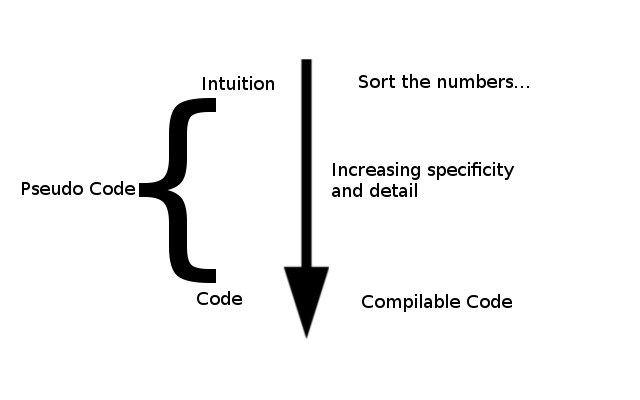
\includegraphics[width=4in]{PseudoCode}
\caption{Pseudo Code gradient range}
\end{figure} 
\section{Insertion Sort}
\textbf{The Iterative Sorting Algorithm}\\
Idea: an array containing all the numbers is traversed with an element
in a placeholder till its appropriate location among the sorted numbers
is found. This is repeated for each of the unsorted numbers until
the array is completely sorted. \\
\begin{figure}[h]
\centering
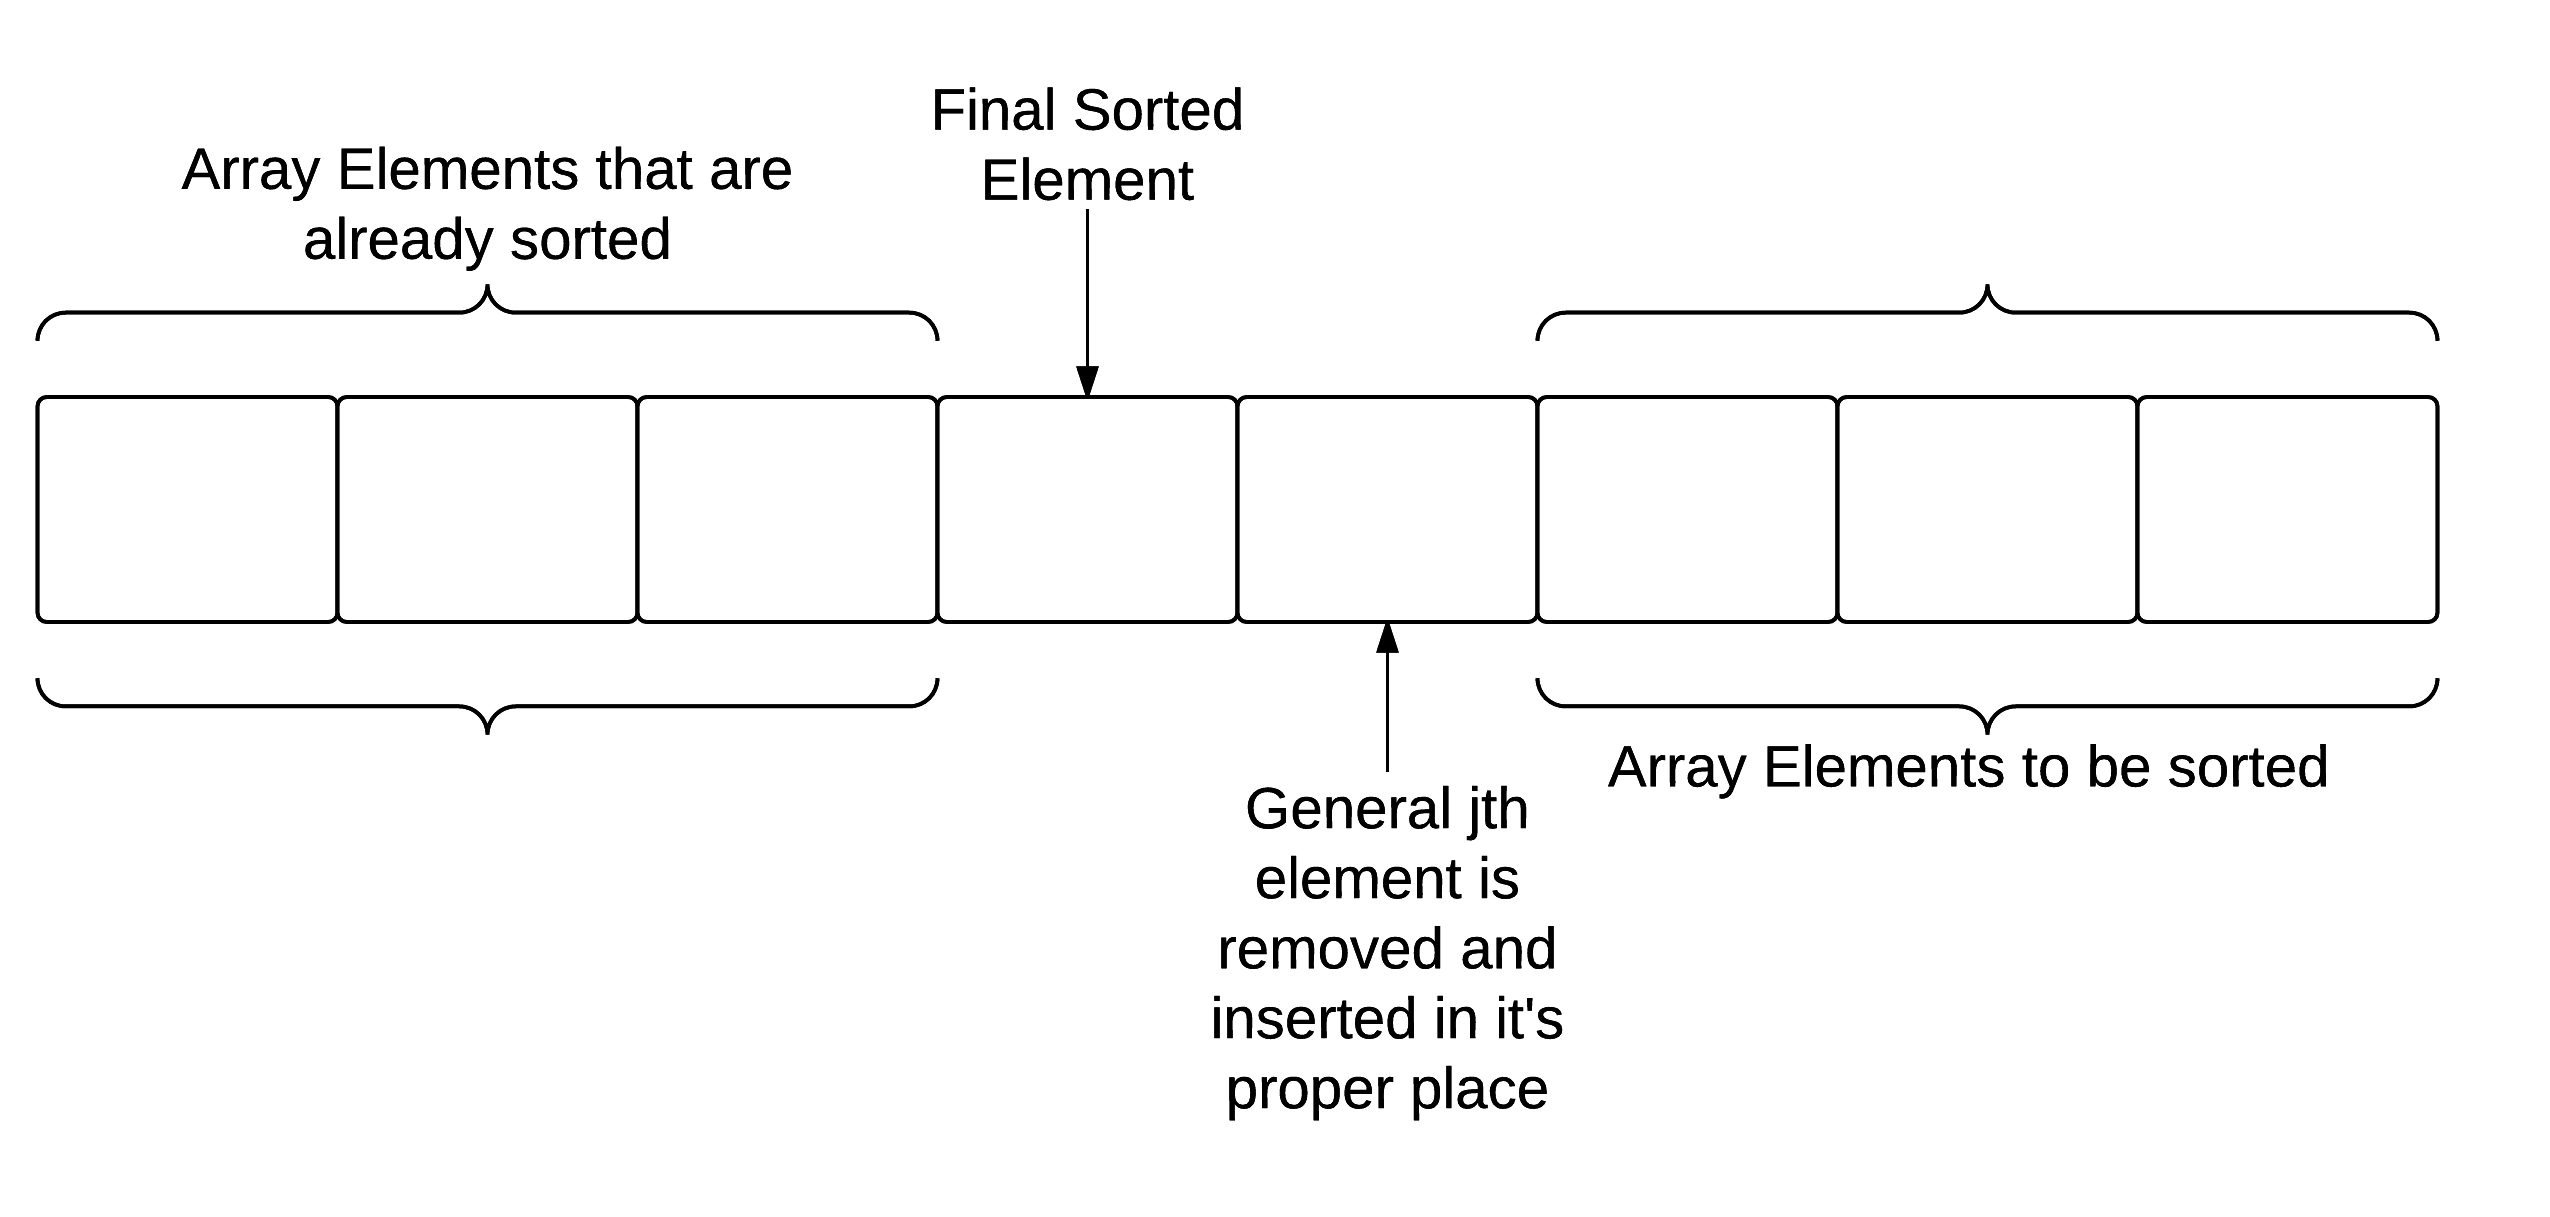
\includegraphics[width=4in]{ISInutition}
\caption{Insertion sort functional intuition}
\end{figure}
\pagebreak
\subsection{Pseudo Code for Insertion Sort}
\begin{algorithm}[h]
\SetAlgoLined
InsertionSort(A, n)\Begin{
	\For {j=2 to n}{
		key=A[j]\;
		i=j-1\;
		\While {$A[i] >$ key and $i > 0$} {
			A[i+1] = A[i]\;
			i = i-1\;
		}
		A[i+1] = key\;
	}
}
\caption{Insertion Sort}
\label{Insertion Sort}
\end{algorithm}
\pagebreak
\subsection{Example: Sort $<52143>$}
First for iteration: j=2 key=2 i=1 \\
A[i] $>$ key $\to <55143> $ \\
i $\ngtr$ 0 $\to$ exit while loop \\
A{[}i{]} = key $<25143>$
\\ \\
Second for iteration: j=3 key=1 i=2 \\
A[i] $ > $key $\to<25543>$ \\
i $> $0 and A[i]$ >$ key $\to<22543>$\\
i $\ngtr$0 exit while$\to <12543>$
\\ \\
Third for iteration j=4 key=4 i=3 \\
A[i] $>$ key $\to<12553>$\\
A{[}i{]} $\ngtr$key exit while $\to<12453>$
\\ \\
Fourth and final for iteration j=5 key=3 i=4\\
A[i] $>$ key $\to<12455>$\\
i $>$ 0 and A[i] $>$ key $\to<12445>$\\
i $>$ 0 but A[i] $\ngtr$key exit while $\to<12345>$\\


\section{Complexity}
Understand the growth of the function's runtime with respect to the size of the arrray i.e. the number of items contained in the array to be sorted, $|n|$. \\
Total runtime isthe sum of the executions of each of the instructions in the code. Each line (i) of code has a runtime $c_i$ which is a known constant and $t_j$ is the number of times that the below "while" loop is executed at the iteration j of the outer for loop.
\begin{figure}[h]
\centering
\begin{tabular}{|l|l|c|c|}
\hline 
Line Number & Pseudocode & Runtime & Number of Executions \\ 
\hline 
  & InsertionSort(A, n) \{ &  &  \\ 
\hline 
1 & \hspace{.5cm}for j=2 to n \{ & $c_1$ & n \\ 
\hline 
2 &  \hspace{.5cm}key=A[j] & $c_2$ & n-1 \\ 
\hline 
3 &  \hspace{.5cm}i=j-1 & $c_3$ & n-1 \\ 
\hline 
4 & \hspace{.5cm} while(i$>$0 and A[i]$>$key)\{ & $c_4$ & $\displaystyle \sum_{j=2}^{n} t_j$ \\ 
\hline 
5 & \hspace{1cm}A[i+1]=A[i] & $c_5$ & $\displaystyle \sum_{j=2}^{n}( t_j-1)$ \\ 
\hline 
6 & \hspace{1cm}i=i-1 & $c_6$ & $\displaystyle \sum_{j=2}^{n}( t_j-1)$ \\ 
\hline 
7 & \hspace{.5cm}\} &  &  \\ 
\hline 
8 & \hspace{.5cm}A[i+1]=key & $c_7$ & n-1 \\ 
\hline 
9 & \} &  &  \\ 
\hline 
\end{tabular}
\caption{Algorithm Complexity Analysis}
\end{figure}

The runtime T(n) is therefore, in this case, given my the following equation:
\[T(n)=c_1 n+c_2 (n-1)+ c_3 (n-1) + c_4  \sum_{j=2}^{n} t_j + c_5 \sum_{j=2}^{n}( t_j-1)+ c_6 \sum_{j=2}^{n}( t_j-1) + c_7 (n-1)\]
In the best possible case, the array is already sorted which implies that $t_j = 1$, leading to the function operating in linear time, which yields the following:
\[T(n)=c_1 n+c_2 (n-1)+ c_3 (n-1) + c_4  \sum_{j=2}^{n} t_j + c_5 \sum_{j=2}^{n}(1-1)+ c_6 \sum_{j=2}^{n}( 1-1) + c_7 (n-1) \] \[ \approx c_1 n+c_2 (n-1)+ c_3 (n-1) + c_4  (n-1) + c_5 n+ c_6 n + c_7 (n-1) \] \[ \approx (c_1 +c_2 + c_3  + c_4  + c_5 + c_6  + c_7 )n\approx c_{net}\cdot n\]
In the worst possible case the array is sorted in reverse order i.e. ascending instead of descending order or vice-versa. This implies that $t_j = j$, leading to the function operating in quadratic time complexity, which yields the following:
\[T(n)=c_1 n+c_2 (n-1)+ c_3 (n-1) + c_4  \sum_{j=2}^{n} j + c_5 \sum_{j=2}^{n}(j-1)+ c_6 \sum_{j=2}^{n}( j-1) + c_7 (n-1) \] \[\approx c_1 n+c_2 (n-1)+ c_3 (n-1) + c_4  \left(\frac{n(n-1)}{2}-1\right) + c_5 \left(\frac{n(n-1)}{2}\right)+ c_6 \left(\frac{n(n-1)}{2}\right) + c_7 (n-1) \]
Following some algebraic manipulation, and combination of constants, the following form demonstrating the quadratic nature of this function's time complexity may be derived.
\[T(n) \approx an^2 + bn + c \]

\subsection{Asymptotic Analysis}
The goal is to compare the performance (runtime) of different algorithms without implementation details. Consider sizes of input which are "sufficiently large". In this situation, the constants are insignificant and therefore irrelevant due to the fact that the leading factor (the highest power of n) determines the complexity.\\

\subparagraph*{Big O Notation} 
The object of this notation and analysis is the asymptotic upper bound of a function. Intuitively it may be thought of in terms of the idea that "The function can do no worse than..." \\
\begin{definition}
Given a function g(n), and n $\in \mathbb{N}$ it is said that\\ $ O(g(n))= f(n)$ if $\exists (c>0 \forall n_0 > 0 ) : 0\leq f(n)\leq cg(n) \forall n \geq n_0$\\
\end{definition}
\begin{figure}[h]
\centering
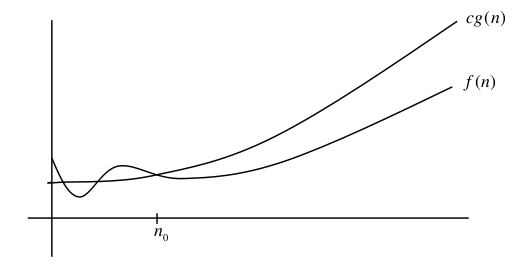
\includegraphics[width=10cm]{bigo}
\caption{Big O relationship graph}
\end{figure}
\pagebreak

\subparagraph*{Example 1:}
$f(n)=3n+3$ Prove $f(n)=O(n)$\\
How to solve? Find values of c and $n_0$ that satisfy the necessary conditions.\\
\[3n+3 \leq cn \hspace{.5cm}\forall \hspace{.5cm} n \geq  n_0 \hspace{1cm}\] divide by n
\[3+ \frac{3}{n} \leq c\]
as n grows, and for all values $>$ 3, $\frac{3}{n} \ll 1$
\[ 3+ small\# \leq c\]
4 is a good candidate - Don't make it more complicated than necessary\\
Solve the remaining inequality for n
\[3n+3\leq4n\]
\[3 \leq n \]
Therefore $n_0$ = 3 and c=4 satisfies the conditions sought to be proven.
 
\subparagraph*{Example 2:}
$f(n)+3n+3$ Prove $f(n)=O(n^2$)
\[3n+3\leq cn^2\]
\[\frac{3}{n}+\frac{3}{n^2} \leq c \to c=2\]
\[3n+3 \leq 2n^2\]
\[2n^2 -3n -3 \geq 0\]
\[n_0 = \left\lceil \frac{3 \pm \sqrt{9-4\cdot 2 \cdot -3}}{4}\right\rceil\  \]
Choose maximum (ceiling) value, so $n_0\approx$5
 
\subparagraph*{Big $\Omega$}is an asymptotic lower bound
\begin{definition}
Given a function g(n), and n $\in \mathbb{N}$ it is said that\\ $ \Omega(g(n))= f(n)$ if $\exists (c>0 \forall n_0 > 0 ) : 0\leq c_1g(n) \leq f(n)\leq c_2g(n) \forall n \geq n_0$\\
\end{definition}
\begin{figure}[h]
\centering
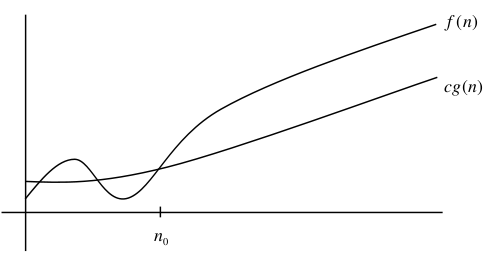
\includegraphics[width=10cm]{bigomega}
\caption{Big $\Omega$ relationship graph}
\end{figure}

\subparagraph{Example 3:}
$f(n) = 2n^2+3$ Prove $f(n)= \Omega$(n)
\[2n^2+3\geq cn \to c=1\]
\[2n^2+3 \geq n \]
\[true \hspace{.5cm} \forall n \geq 0\]
\[\therefore n_o=0\]

\subparagraph{Example 4:}
$f(n) = 2n^2+3$ Prove $f(n)= \Omega(n^2)$
\[2n^2+3\geq cn \to c=1\]
\[2n^2+3 \geq n \]
\[true \hspace{.5cm} \forall n \geq 0\]
\[\therefore n_o=0\]

\subparagraph*{Big $\Theta$}is an asymptotic tight bound
\begin{definition}
Given a function g(n), and n $\in \mathbb{N}$ it is said that\\ $ \Theta(g(n))= f(n)$ if $\exists (c_1, c_2>0 \forall n_0 > 0 ) : 0\leq c_1g(n) \leq f(n)\leq c_2g(n) \forall n \geq n_0$\\
\end{definition}
\begin{figure}[h]
\centering
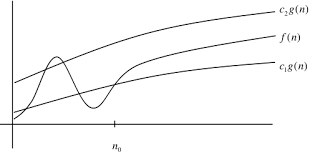
\includegraphics[width=10cm]{bigtheta}
\caption{Big $\Theta$ relationship graph}
\end{figure}

\subparagraph{Example 5:}
$f(n) = \frac{n^2}{2}-3n$ Prove $f(n)= \Theta(n^2)$
\[c_1n^2 \leq \frac{n^2}{2}-3n \leq c_2n^2\]
\[c_1 \leq \frac{1}{2}-\frac{3}{n} \leq c_2 \]
\[\forall n \geq 12 \to c_1=\frac{1}{4}, c_2=1\]
\[\frac{1}{4}n^2 \leq \frac{n^2}{2}-3n \leq n^2\]
\[true \hspace{.5cm} \forall n \geq 12\]
\[\therefore n_o=12,\hspace{.5cm} c_1=\frac{1}{4},\hspace{.5cm} c_2=1 \]

\begin{figure}[h]
\centering
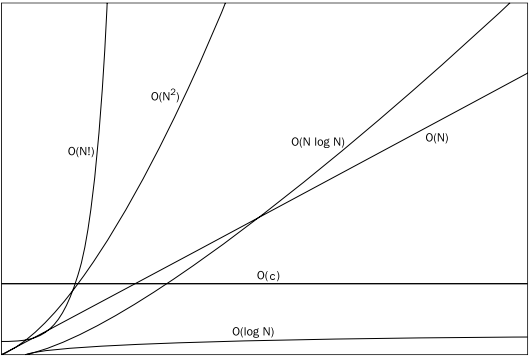
\includegraphics[width=10cm]{bigofun}
\caption{Common complexities graphed concurrently}
\end{figure}
\subsection{Algebra of Asymptotic Notation}
\begin{definition}[Interrelationship of O $\Omega$ and $\Theta$]\hfill \break
given f(n) and g(n)\\ f(n)=$\Theta$(g(n)) iff f(n)=$\Omega$(g(n)) and f(n)=O(g(n)) 
\end{definition}
\begin{definition}[Constants]\hfill \break
$\forall$ k $\in \mathbb{R^+}$ \\
if f(n)=O(g(n)) then kf(n)=O(g(n))\\
which implies constants have no effect \\
also applies to $\Theta$ as well as $\Omega$
\end{definition}

\begin{definition}[Sums]\hfill \break
if f(n)=O(g(n)) AND d(n)=O(h(n))\\
then f(n)+d(n)=O(g(n)+h(n))=O(max[g(n), h(n)])\\
also applies to $\Theta$ as well as $\Omega$\\
Note: Hidden Constants - Algorithms exist that have better efficiency only at extreme limits (i.e. Counting Sort)
\end{definition}

\begin{definition}[Multiplication]\hfill \break
if f(n)=O(g(n)) AND d(n)=O(h(n))\\
then f(n)$\cdot$d(n)=O(g(n)$\cdot$h(n))\\
also applies to $\Theta$ as well as $\Omega$\\
\end{definition}

\begin{definition}[Transitivity]\hfill \break
if f(n)=O(g(n)) AND g(n)=O(h(n))\\
then f(n)=O(h(n))\\
also applies to $\Theta$ as well as $\Omega$\\
\end{definition}

\begin{definition}[Reflexivity]\hfill \break
f(n)=O(f(n))\\
also applies to $\Theta$ as well as $\Omega$\\
\end{definition}

\begin{definition}[Symmetry]\hfill \break
iff f(n)=$\Theta$(g(n)) then g(n)=$\Theta$(f(n))\\
iff f(n)=O(g(n)) then g(n)=$\Omega$(f(n))\\
iff f(n)=$\Omega$(g(n)) then g(n)=O(f(n))\\
\end{definition}

\section{The Search Problem}
Searching an ordered sequence: Given an ordered sequence $<a_1, a_2, ... a_n>$ and a value $x$, determine if $x$ is in the sequence or not. \\
Trivial Solution: Iterate through the whole sequence: O(n)\\
Better Solution: Binary Search\\
Binary search is a recursive function in the base case, the array is of length 1, if that element is equal to $x$ return True, else return False. Its recursive step is executed when the array is longer than a single element. 
\begin{figure}[h]
\centering
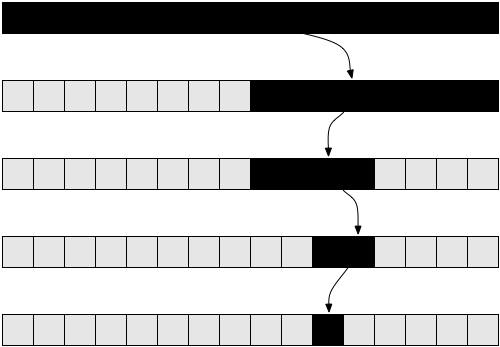
\includegraphics[width=5cm]{binsearch}
\caption{Binary Search Execution}
\end{figure}

\subsection{Pseudo Code for Binary Search}
\begin{algorithm}[h]
BinarySearch(A, start, end)\Begin{ //(A, 1, n) for first call\\
	\If {start==end} {
		\If {A[start]==x} {
			return True
		}
		return False		
	}
	m=$\left \lceil \frac{start+end}{2} \right\rceil$\\
	\If {A[m] $>$ x}{
		return BinarySearch(A, start, m-1)
	}
	return BinarySearch(A, m, end)
}

\caption{Binary Search}
\label{Binary Search}
\end{algorithm}
\FloatBarrier
\subsection{Example: Search $<1,3,7,9,11>$ for x=9}
First call: start=1 end =5\\
start $\ne$ end $\to$ m=$\left \lceil\frac{5+1}{2}\right\rceil=3$ $\to$ A[3]=7$\ngtr$x \\recursive call BinarySearch(A, m, end)\\ \\
Second call: start=3 end=5\\
start $\ne$ end $\to$ m=$\left \lceil\frac{5+3}{2}\right\rceil=4$ $\to$ A[4]=9$\ngtr$x \\recursive call BinarySearch(A, m, end)\\ \\
Third call: start=4 end=5\\
start $\ne$ end $\to$ m=$\left \lceil\frac{5+4}{2}\right\rceil=5$ $\to$ A[5]=11$>$x \\recursive call BinarySearch(A, start, m-1)\\ \\
Fourth call: start=4 end=4\\
start = end $\to$ A[4]=9==x \\return True\\ \\

\section{Recurrence Equations}
\[T(n)=\begin{cases}base \hspace{.5cm} \Theta(1) & n=1 \\ recursive \hspace{.5cm} T(\frac{n}{2})+\Theta(1) & n>1\end{cases}\]
Recursive Tree method:
\begin{itemize}
\item Nodes represent the cost of a single sub-problem at that level of recursion
\item Each level of the tree is a level of recursion
\item Between the root and leaves, but excluding the root and leaves, are intermediate recursive calls
\item Leaves are the base cases
\item Normally, write three specific levels then find the general level expression
\item Unless otherwise specified all logarithms are assumed to be $log_2$
\end{itemize}
\subsection{Example based on the above recurrence equation:}
\begin{figure}[h]
\centering
\begin{tabular}{|c|c|c|c|}
\hline
Tree & Level & Input Size & Cost\\
\hline
\hline
c & 0 & n & c\\
\hline
c & 1 & $\frac{n}{2}$ & c\\
\hline
c & 2 & $\frac{n}{4}$ & c\\
\hline
c & i & $\frac{n}{2^i}$ & c\\
\hline
c & k (leaf or base case) & $\frac{n}{2^k}=1$ & c\\
\hline
\end{tabular}
\caption{Recursion Tree table basic example}
\end{figure}  
Solve for k which represents the level at which the base case is reached:
\[ 1 = \frac{n}{2^k} \]
\[2^k=n\]
\[k=log_2 (n)\]
Use this to find the total runtime:
\[\sum_{i=0}^{k-1}c+c=\sum_{i=0}^{log(n)-1}c+c=c\cdot log(n)+ c = \Theta(log(n))\]
\subsection{Example:}
Recurrence Equation:
\[T(n)=\begin{cases}2T(\frac{n}{2})+\Theta(n^2) & n>1\\ \Theta(1) & n=1\end{cases}\]
\begin{figure}[h]
\centering
\begin{tabular}{|c|c|c|c|}
\hline
Tree & Level & Input Size & Cost\\
\hline
\hline
$c(n^2)$ & 0 & n & $c(n^2)$\\
\hline
$c(n^2)\hspace{.5cm}c(n^2)$ & 1 & $\frac{n}{2}$ & $\frac{c(n^2)}{2}$\\
\hline
$ c(n^2) \hspace{.5cm} c(n^2) \hspace{.5cm} c(n^2)\hspace{.5cm}c(n^2)$ & 2 & $\frac{n}{4}$ &  $\frac{c(n^2)}{4}$\\
\hline
$c(n^2)\hspace{.5cm}...\hspace{.5cm}c(n^2)$ & i & $\frac{n}{2^i}$ & $\frac{c(n^2)}{2^i}$\\
\hline
$\Theta(1)\hspace{.5cm}...\hspace{.5cm}\Theta(1)$ & k (leaf or base case) & $\frac{n}{2^k}=1 \to k=log(n)$ & $c\cdot 2^k\Theta(1)$\\
\hline
\end{tabular}
\caption{Recursion Tree table example}
\end{figure}\\ \\
\[\sum_{i=0}^{log(n)-1}c+c=c\frac{n^2}{2^i}+cn = cn^2\sum_{i=0}^{log(n)-1}(\frac{1}{2})^i+cn\]
use the summation expression property for geometric series
\[ \sum_{i=0}^{\infty} x^i=\frac{1}{1-x}\hspace{.5cm} \forall x<1\]
employed in our case:
\[cn^2\sum_{i=0}^{log(n)-1}(\frac{1}{2})^i+cn=2cn^2+cn=\Theta(n^2)\]

\section{The Master Theorem}
(or, how to solve recurrence problems without trees)\\ \\
Let $a\ge1$, and $b\ge1$ be constants and $f(n)$ be a function.\\ Consider $T(n)=aT(\frac{n}{b})+f(n)$. This leads to three cases.

\begin{enumerate}
\item if $f(n)=O(n^{log_b(a)-\varepsilon})$ for some $\varepsilon > 0$\\
	then you may conclude that $T(n)=\Theta(n^{log_b(a)})$
\item if $f(n)=\Theta(n^{log_b(a)})$ \\
	then you may conclude that $T(n)=\Theta(n^{log_b(a)}log(n))$
\item if $f(n)=\Omega(n^{log_b(a)+\varepsilon})$ for some $\varepsilon > 0$ \\and if $af(\frac{n}{b})\le cf(n)$ for $c<1$ and sufficiently large $n$\\
	then you may conclude that $T(n)=\Theta(f(n))$ 
\end{enumerate}

\subsubsection{Master Theorem Examples: Case 1 illustration}
\[T(n)=9T(\frac{n}{3})+n  \to \quad a=9 \quad b=3 \quad f(n)=n\]
\[n^{log_b(a)}=n^{log_3(9)}=n^2 \to f(n)=O(n^{2-\varepsilon}) \quad \forall \quad 0 < \varepsilon \le 1 \]
Therefore this example falls into case 1 and
\[T(n)=\Theta(n^{log_b(a)})=\Theta(n^{log_3(9)})=\Theta(n^2)\]
\subsubsection{Case 2 illustration}
\[T(n)=9T(\frac{2n}{3})+1  \to \quad a=1 \quad b=\frac{3}{2} \quad f(n)=1\]
\[n^{log_b(a)}=n^{log_{\frac{3}{2}}(1)}=n^0 \because any \quad log_x(1)=0 \to f(n)=\Theta(n^0) =\Theta(1) \]
Therefore this example falls into case 2 and
\[T(n)=\Theta(n^0log(n))=\Theta(log(n))\]
\subsubsection{Case 3 illustration}
\[T(n)=3T(\frac{n}{4})+nlog(n)  \to \quad a=3 \quad b=4 \quad f(n)=nlog(n)\]
\[n^{log_b(a)}=n^{log_4(3)}=n^0.7925 \to f(n)=\Omega(n^{.7925-\varepsilon}) \quad for \quad \varepsilon = 0.2 \]
\[and \quad af(\frac{n}{b})=3f(\frac{n}{4})=3\frac{n}{4}log(\frac{n}{4}) \quad \therefore af(\frac{n}{b}) \le cf(n)\]
Therefore this example falls into case 3 and
\[T(n)=\Theta(nlog(n))\]
\section{Divide and Conquer}
\begin{enumerate}
\item Divide: Find a way to separate sub-problems out of the original. Ideally, they should be smaller instances of the same fundamental problem.
\item Conquer: If the size of the problem is small enough solve it in a straightforward way, or, if the problem is not small enough, solve the sub-problem recursively.
\item Combine: Put together the solutions of the sub-problems in a way that yields the solution to the main problem 
\end{enumerate}
\subsection{Merge Sort: The Recursive sorting algorithm}
\begin{enumerate}
\item Divide: Break up the sequence of n elements into two smaller sub-sequences of length $\frac{n}{2}$
\item Conquer: If the sub-sequences have length one, they are sorted, if they have a length greater than one, recursively sort the sub-sequences.
\item Combine: Bring together the sorted sub-sequences in a manner that sorts them to obtain the original array, now sorted.
\end{enumerate}
\begin{algorithm}
MergeSort(A, start, end)\Begin{
	\If {start$<$end}{
		m=$\left \lfloor \frac{start+end}{2}\right\rfloor$\\
		MergeSort(A, start, m)\\
		MergeSort(A, m+1, end)\\
		Merge(A, start, m, end)\\
	}
}
\caption{Merge Sort}
\label{Merge Sort}
\end{algorithm}
\begin{algorithm}[H]
Merge(A, start, m, end)\Begin{//Linear Compleity i.e. $\Theta(n)$\\
i=start\\
j=m+1\\
k=1\\
create an array B of length end-start+1\\
\While{i$\le$m and j$\le$end}{
	\If {A[i]$<$}{
		B[k]=A[i]\\
		k++\\
		i++\\
	}\Else{
		B[k]=A[j]\\
		k++\\
		j++\\
	}
}
\While{i$\le$m}{
	B[k]=A[i]\\
	i++\\
	k++\\
}
\While{j$\le$end}{
	B[k]=A[j]\\
	j++\\
	k++\\
}
Copy B in A
}
\caption{Merge}
\label{Merge}
\end{algorithm}
\pagebreak

\begin{figure}[h]
\centering
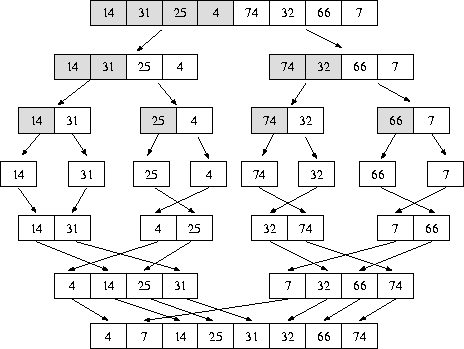
\includegraphics[width=8cm]{mergesort}
\caption{Merge Sort Execution}
\end{figure}
\subsection{Merge Sort Complexity}

\[T(n) = \begin{cases} 2T(\frac{n}{2})+\Theta(n) & n>1 \\ \Theta(1) & n=1 \end{cases}\]
\subparagraph{Recursion Tree Method:} \quad \\
\begin{figure}[h]
\centering
\begin{tabular}{|c|c|c|c|}
\hline
Tree & Level & Input Size & Cost\\
\hline 
\hline
$cn$ & 0 & $n$ & $cn$ \\ \hline
$\frac{cn}{2}$ \quad $\frac{cn}{2}$ & 1 & $\frac{n}{2}$ & $cn$ \\ \hline
$\frac{cn}{4}$ \quad $\frac{cn}{4}$ \quad $\frac{cn}{4}$ \quad $\frac{cn}{4}$ & 2 & $\frac{n}{4}$ & $cn$ \\ \hline
$\frac{cn}{2^i} \quad \cdots \quad \cdots \quad \frac{cn}{2^i}$ & i & $\frac{n}{2^i}$ & $cn$ \\ \hline
$\Theta (1) \quad \cdots \quad \cdots \quad \Theta (1)$ & k & $1=\frac{n}{2^k} \quad k=log_2(n) $ & $ 2^k$ \\ \hline
\end{tabular}
\caption{Merge Sort Complexity Analysis: Recursion Tree Method}
\end{figure}
$$ \sum_{i=0}^{log(n)-1}cn+c2^k=cn\sum_{i=0}^{log(n)-1}1+c2^{log_2(n)}=cnlog(n)+cn^{log_2(2)}=\Theta(nlog(n)) $$
\subparagraph{Master Theorem:} a=2 b=2 f(n)=$\Theta(n)$
\[n^{log_b(a)}=n^{log_2(2)}=n^1=n\]
\[case \quad 2 \because f(n)=\Theta(n^{log_2(2)})=\Theta(n)=f(n)\]
\[ \therefore T(n)=\Theta(nlog(n))\]
\subsection{Another Complexity Example}
$$T(n) = \begin{cases} 16T(\frac{n}{4})+\Theta(n) & n>1 \\ \Theta(1) & n=1 \end{cases}$$
\subparagraph{Recursion Tree Method} \quad \\
\begin{figure}[h]
\centering
\begin{tabular}{|c|c|c|c|}
\hline
Tree & Level & Input Size & Cost\\
\hline 
\hline
$cn$ & 0 & $n$ & $cn$ \\ \hline
$\frac{cn}{4} \cdots (16) \cdots \frac{cn}{4}$ & 1 & $\frac{n}{4}$ & $4cn$ \\ \hline
$\frac{cn}{16} \cdots (16^2) \cdots \frac{cn}{16}$ & 2 & $\frac{n}{16}$ & $16cn$ \\ \hline
$\frac{cn}{4^i} \cdots (16^i) \cdots \frac{cn}{4^i}$ & i & $\frac{n}{2^i}$ & $4^icn$ \\ \hline
$\Theta (1) \cdots (16^k) \cdots \Theta (1)$ & k & $1=\frac{n}{4^k} \quad k=log_4(n) $ & $ c16^k = c16^{log_4(n)}=cn^{log_4(16)}=cn^2$ \\ \hline
\end{tabular}
\caption{Complexity Analysis: Recursion Tree Method}
\end{figure}
$$ \sum_{i=0}^{log(n)-1}4^icn+c16^k=cn\sum_{i=0}^{log(n)-1}4^i+cn^2 $$
To solve summation recall:
$$ \sum_{i=0}^{k}z^i=\frac{z^{k+1}-1}{z-1} $$
Implemented here:
$$ cn\sum_{i=0}^{log(n)-1}4^i+cn^2 =cn\frac{4^{log_4(n)-1+1}-1}{4-1} $$
Absorb denominator into general constant
$$ cn\cdot n^{log_4(4)=1}-cn+cn^2=cn^2+cn^2-cn=\Theta(n^2)  $$
\subsection{Maximum Subarray Problem}
Given an array of size n containing positive and negative numbers find the subarray with the maximum sum of elements: \\
\begin{figure}[h]
\centering
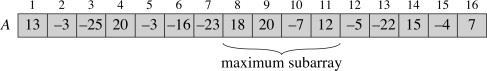
\includegraphics[width=10cm]{maxsubarray}
\end{figure} \\
\begin{itemize}
\item Really dumb solution: Consider the first element and all possible subarrays beginning with that element summing each of these along the way until it proceeds to the next element and repeats all the calculations = $\Theta(n^3)$ 
\item Straightforward (and inefficient) solution: Try every subarray and find the maximum = $\Theta(n^2)$
\item Divide and Conquer Algorithm: allows the problem to be solved in $\Theta(nlog(n))$
\end{itemize}
\subparagraph{Divide and Conquer approach}
\begin{itemize}
\item Let i and j be the beginning and end of a subarray with max sum
\item If the max subarray is on the left side, both i and j are on the left, $ start \leq i \leq j \leq m \leq end $
\item If the max subarray is on the right side, both i and j are on the right, $ start \leq m+1 \leq i \leq j \leq end $
\item If the max subarray crosses m it has elements on the left and right of m, $ start \leq i \leq m \leq j \leq end $
\end{itemize}
\begin{figure}[h]
\centering
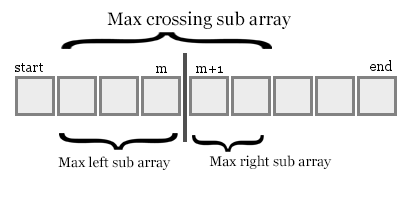
\includegraphics[width=10cm]{maxcrosssubarraysme}
\end{figure}
\begin{algorithm}[htb!]
\SetAlgoLined
FindMaxCrossingSubarray(A, start, m, end)\Begin{ \quad // $\Theta(n)$ \\
	lsum=-$\infty$ //sum of max left subarray ending with m \\
	maxl //index of element that begins the max subarray\\
	sum=0 \\
	\For { i=m down to start}{
		sum = sum+A[i]\\
		\If {lsum<sum}{
			lsum=sum\\
			maxl=i\\
		}
	}
	rsum=-$\infty$ \\
	maxr \\
	sum=0 \\
	\For { j=m+1 end}{
		sum = sum+A[j]\\
		\If {rsum<sum}{
			rsum=sum\\
			maxr=i\\
		}
	}
	return (maxl, maxr, lsum+rsum)\\
}
\caption{FindMaxCrossingSubarray}
\label{FindMaxCrossingSubarray}
\end{algorithm}
\begin{algorithm}[htb!]
\SetAlgoLined
FindMaxSubarray(A, start, end)\{ \\
\If {start==end}{ return (start, end, A[start])}
m=$ \left \lfloor \frac{start+end}{2} \right \rfloor$\\
(lstart, lend, lsum)=FindMaxSubarray(A, start, m)\\
(rstart, rend, rsum)=FindMaxSubarray(A, m+1, end)\\
(cstart, cend, csum) = FindMaxCrossingSubarray(A, start, m, end)\\
\If{lsum$\geq$rsum and lsum$\geq$csum}{return(lstart, lend, lsum}
\If{rsum$\geq$lsum and rsum$\geq$csum}{return(rstart, rend, rsum}
return(cstart, cend, csum)\\
\}
\caption{FindMaxSubarray}
\label{FindMaxSubarray}
\end{algorithm}
\pagebreak
\subparagraph{FindMaxSubarray Complexity by Master Theorem}
\[ T(n)=\begin{cases} 2T(\frac{n}{2})+\Theta(n) & n>1 \\ \Theta(1) & n=1 \end{cases} \]
\[a=2 \quad b=2 \quad f(n)=n\]
\[ n^{log_2(2)}=n \quad f(n)=n=\Theta(n)\quad \therefore case \quad 2 \]
\[T(n)=\Theta(nlog(n))\]
\subsection{QuickSort}
Quicksort applies the divide and conquer approach to the sorting problem. The internal constants are known and proven to be small which implies that Quicksort is one of the best solutions in practical situations. In each successive recursive call one element is placed in the proper position and is called a pivot. 
\begin{itemize}
\item Divide: given the array A[start..end] choose a value for the pivot x such that A[p]=x alter the array so both of the following statements hold:\\
\[ \forall i \in [start...p-1] \quad A[i]\leq x \]
\[ \forall i \in [p+1...end] \quad A[i] > x \]
\item Conquer: Recursively sort the left and right sides of x. The subarrays A[start...p-1] and A[p+1...end]
\item Combine: Nothing left to do. The array is already sorted.
\end{itemize}
\begin{algorithm}
QuickSort(A, start, end)\Begin{
\If{start$<$end}{
	p=Partition(A, start, end)\\
	QuickSort(A, start, p-1)\\
	QuickSort(A, p+1, end)
}
}
\caption{QuickSort}
\label{QuickSort}
\end{algorithm}
\begin{algorithm}
Partition(A, start, end)\Begin{
x=A[end]\\
i=start-1\\
\For{j=start to end}{
	\If{A[j]$\leq$x}{
		i++\\
		swap(A[i], A[j])\\
	}
}
swap(A[i+1], A[end])\\
return i+1\\
}
\caption{Partition}
\label{Partition}
\end{algorithm}
\begin{figure}[htb!]
\centering
\includegraphics[width=13cm]{quicksortbetter}
\caption{Execution of QuickSort on an array}
\end{figure}
\subparagraph{Complexity of QuickSort}
Assume an array of length n
\[T(n)=\begin{cases}T(k)+T(n-k-1)+\Theta(n) & n>1 \\ \Theta(1) & n=1 \end{cases}\]
Worst case: x is the min $\to$ k=0 or x is the max $\to$ k=n-1 then Quicksort=$\Theta(n^2)$:
\[T(n)=\begin{cases} \cancel{T(0)} +T(n-1)+\Theta(n) & n>1 \\ \Theta(1) & n=1 \end{cases}\]
Best case: k is the index of the median array element i.e. k$\approx\frac{n}{2}$ then QuickSort=$\Theta(nlog(n))$:
\[T(n)=\begin{cases}2T(\frac{n}{2})+\Theta(n) & n>1 \\ \Theta(1) & n=1 \end{cases}\]
\subsection{Counting Sort}
Counting Sort achieves sorting in linear time. The basic idea is, based on the assumption that the array to be sorted is of size n, and its maximum integer is k, CountingSort counts the number of distinct elements and this count determines the position of each element in the output array.
\begin{enumerate}
\item Create new array
\item Fill out the new counting array with the number of occurrences of each element
\item Update the counting array cumulatively, adding up occurrences 
\end{enumerate}
In the context of the following pseudocode, A is the input array, B is the output array, n is the number of elements in the array, and k is the maximum value of any individual array element.
\begin{algorithm}
CountingSort(A, B, n, k)\Begin{
	Let C[0...k] be a new array\\
	\For {i=0 to k}{
		C[i]=0	
	}
	\For{j=1 to n}{
		C[A[j]]=C[A[j]]+1
	}
	\For {i=1 to k}{
		C[i]=C[i]+C[i-1]
	}
	\For {j=n to 1}{
		B[C[A[j]]]=A[j]
		C[A[j]]=C[A[j]]-1
	}
}
\label{CountingSort}
\caption{CountingSort}
\end{algorithm}
\begin{figure}[htb!]
\centering
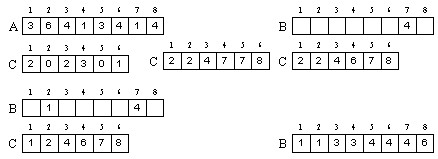
\includegraphics[width=10cm]{countingsort}
\caption{CountingSort Execution}
\end{figure}
\pagebreak
\part{Iterative Problem Solving}
This strategy relies on the decomposition of the main problem into subproblems, but in a different manner than in the Divide and Conquer approach. This is particularly advantageous when subproblems are overlapped.
\subsection{Examples}
\subparagraph{Fibonacci}
In the Fibonacci sequence, each successive value is based on both of the two preceding values, and nothing else. 
\[F(x)=\begin{cases}0 & x=0 \\ 1 & x=1 \\ F(n-1)+F(n-1) & x\geq 2 \end{cases}\]
\subparagraph{Matrix Multiplication} Given a matrix A 100x1, a matrix B 1x50, and a matrix C 50x2, consider the following cases:
\[A(BC)\to (100x1)((1x50)(50x2))\]
This series of multiplications includes the first parenthetical resolution requires 100 multiplication operations and then a further 200 multiplication operations, for a total of 300 multiplication operations to perform this calculation.
\[(AB)C \to ((100x1)(1x50))(50x2) \]
This series of multiplications is very different. The first resolution here requires 5,000 multiplication operations, and the second 10,000, for a total of 15,000 multiplication operations necessary in total. In both cases, the end result result is a 100x2 matrix, but the cost in time is vastly different. 
\section{Greedy Algorithms}
Greedy Algorithms are useful in a wide array of cases, especially dealing with optimization problems defined in a particular domain. These are commonly problems of maximizing or minimizing some system parameter or variable. They are generally iterative approaches, and at each iteration the algorithm makes the "best" currently available decision according to its selection criteria. Greedy Algorithms do not always find the optimal solution to a problem. \\
There are a set of conditions which are both necessary and sufficient for a problem to be optimally solved by a greedy algorithm. \\
If a greedy algorithm does not solve a problem optimally, often it provides a bounded solution with respect to the optimal solution.\\
Greedy Algorithms build a partial solution which is extended at each iteration, and it never changes it's mind. 
\subsection{The Activity Selection Problem}
\begin{itemize}
\item Consider n activities $\in$ A=[$a_1 \cdots a_n$] from which a subset should be selected to occur in one classroom
\item Each activity has a start and finish time
\item The $i^{th}$ activity has a start time $s_i$ and a finish time $f_i$ such that $0\leq s_i < f_i < \infty$.
\item When an activity is scheduled, it takes place in the open interval $[s_i, f_i)$
\item Two activities $a_1=[s_i, f_i)$ and $a_2=[s_j, f_j)$ are compatible if they do not overlap ie: $s_i \geq f_j$ or $s_j \geq f_i$
\end{itemize}
Problem: Given the activities in A, select the maximum number of compatible activities. Consider the following diagram representing the set of activities A.
\begin{figure}[htb!]
\centering
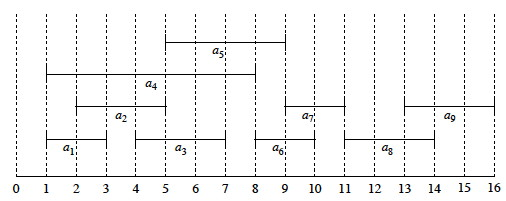
\includegraphics[width=12cm]{greedyactivity}
\caption{Example of a list of activities to which this Greedy algorithm may be applied}
\end{figure}
In this example, one optimal, but not the only optimal, solution would consist of the activities $\{a_1, a_3, a_6, a_8\}$. In any solution, given this set of activities, the maximal number which may be compatible is 4. Therefore any solution which consists of exactly 4 compatible activities is optimal. If instead the desired parameter to be optimized is amount of class time allocated, the problem becomes considerably more complex, and in fact cannot be solved in polynomial time.
\subparagraph{The Greedy Approach - Exploring criteria:}
Iteratively build a set s which consists of compatible activities. The set s is extended at each iteration. In each iteration which activity should be selected? What should be the criteria by which the greedy algorithm makes its choice?
\begin{enumerate}
\item Earliest start time
\item Least duration
\item Earliest termination time
\item least conflicting activities
\end{enumerate}
\begin{algorithm}[h]
EarliestStart(A)\Begin{
S=$\emptyset$ //the null or empty set \\
\While{$\exists$ a $\in$ A : S $\cup \{a\}$ does not create overlaps}{
	D=subset of (A-S) that do not overlap with activities in S\\
	$a_k$ = $\underset{a_i\in D}{\arg\min}$ $s_i$\\
	S=S$\cup\{a_k\}$\\
}
return S\\
}
\caption{Earliest Start time as greedy criteria}
\label{Early Start Greedy}
\end{algorithm}
\subparagraph{Counter Examples to Earliest Start} Consider the following set of activities: \\
\begin{figure}[h]
\centering
\begin{tabular}{|c|c|}
\hline
$a_1$ & [1,10)\\ \hline
$a_2$ & [2,3)\\ \hline
$a_3$ & [4,5)\\ \hline
\end{tabular}
\caption{Activity set to serve as counterexample to EarliestStart}
\end{figure}\\
With the greedy criteria being earliest start, $a_1$ alone is chosen, since it conflicts with both of the other two potential activities. If one of the other activities had been chosen a max of two activities could have been selected. This selection criteria therefore does not lead to an optimal solution, proven by counter example.
\begin{algorithm}[h]
LeastDuration(A)\Begin{
S=$\emptyset$ //the null or empty set \\
\While{$\exists$ a $\in$ A : S $\cup \{a\}$ does not create overlaps}{
	D=subset of (A-S) that do not overlap with activities in S\\
	$a_k$ = $\underset{a_i\in D}{\arg\min}$ $(f_i-s_i)$ //This is the only altered line\\
	S=S$\cup\{a_k\}$\\
}
return S\\
}
\caption{Least Duration as greedy criteria}
\label{Shortest Greedy}
\end{algorithm}
\subparagraph{Counter Examples to Earliest Start} Consider the following set of activities: \\
\begin{figure}[h]
\centering
\begin{tabular}{|c|c|}
\hline
$a_1$ & [5,7)\\ \hline
$a_2$ & [3,6)\\ \hline
$a_3$ & [6,9)\\ \hline
\end{tabular}
\caption{Activity set to serve as counterexample to LeastDuration}
\end{figure}\\
With the greedy criteria being least duration, $a_1$ alone is again chosen, since it conflicts with both of the other two potential activities. If one of the other activities had been chosen a max of two activities could have been selected. This selection criteria therefore does not lead to an optimal solution, proven by counter example.
\begin{algorithm}[h]
EarliestTermination(A)\Begin{
S=$\emptyset$ //the null or empty set \\
\While{$\exists$ a $\in$ A : S $\cup \{a\}$ does not create overlaps}{
	D=subset of (A-S) that do not overlap with activities in S\\
	$a_k$ = $\underset{a_i\in D}{\arg\min}$ $f_i$\\
	S=S$\cup\{a_k\}$\\
}
return S\\
}
\caption{Earliest Finish time as greedy criteria}
\label{Early Finish Greedy}
\end{algorithm}
\subparagraph{Earlier Counter Examples Handled} Consider the following set of activities: \\
\begin{figure}[h]
\centering
\begin{tabular}{|c|c|c|}
\hline
\quad & Set 1 & Set 2 \\ \hline
$a_1$ & [1,10) & [5,7) \\ \hline
$a_2$ & [2,3) & [3,6) \\ \hline
$a_3$ & [4,5) & [6,9)\\ \hline
\end{tabular}
\caption{Activity set to serve as counterexample to EarliestStart}
\end{figure}\\
For Set 1 and Set 2, with the other criteria, only one activity ($a_1$) could be selected, but here, since $a_2$ has the earliest termination time it is selected first, and in the next iteration, $a_3$ is selected which is the only other available, non-conflicting activity. It yields an optimal solution, in both cases.\\
\subsection{Greedy Algorithm Correctness}
The proof of correctness for a greedy algorithm is a multistage process, but three main steps are required.
\begin{enumerate}
\item Termination - Prove that for any input, it will complete a finite number of steps
\item Partial Solution Correctness - Prove that the partial solution built at every iteration is included in the optimal solution. This is normally achieved through a proof by induction. 
\item Demonstrate that the final solution is optimal 
\end{enumerate}
\subparagraph{Application to Earliest Termination}
\begin{enumerate}
\item We add a new activity in s at every iteration of the loop so we can have, at most, $|A|$ iterations.
\item \underline{Base}: (h=0) $0^{th}$ iteration this implies that $S_0= \emptyset = \{\}$. The empty set is a subset of any set so $S_0 \subset S^*$ $\forall$ optimal solution $S^*$\\ 
\underline{Assume}: at iteration $h>0$ $S_h \subset S^*$ \\
\underline{Inductive Step}: There exists an optimal solution such that $S_{h+1}$ is a subset of it. \\
At iteration h+1, $S_{h+1}=S_h\cup{a_k}$\\
If $a_k\in S^*$ then $S_{h+1}\subseteq S^* \to$ done\\
If $a_k\notin S^*$ then $S_{h+1}\nsubseteq S^* \to$ \\ 
It must therefore be proven that there exists a different optimal solution $S^\#$ such that $S_{h+1} \subseteq S^\#$
\underline{Facts}:
\begin{itemize}
\item $S_{h+1}$ does not contain overlaps 
\item $|S^*|\geq |S_{h+1}|\to \exists a_j \in S^* \wedge \notin S_{h+1}$
\item Let $a_j \in \{ S^* \setminus S_{h+1}\}$ be the activity with the earliest termination time
\item $a_j \in S_h $ also $S_h \subseteq S^*$ and $a_j \in S^\#$ and $S^*$ does not contain overlaps
\item Therefore $a_j$ does not create overlaps with activities in $S_h$ and would have been selected, but the algorithm selected $a_k \therefore f_k\leq f_j$
\item $S^\#=\{S^* \setminus \{a_j\} \cup \{ a_k \} \} $
\item this does not contain overlapp becuse $a_k$ has the same or earlier finish time than $a_j$
\item Therefore $S^\#$ is optimal if $S^*$ is because $|S^\#|=|S^*|$
\end{itemize}
\item Demonstrate final Solution is optimal:\\
Let m be the number of iterations of the while loop.\\
Proof by contradiction:\\
\[\exists S^* : S_m \subseteq S^* \]
Assume falsity of the prior statement 
\[|S_m|<|S^*|\]
\[\exists a: a \in S^* \wedge a \notin S_m\]
Therefore a is compatible with every activity in $S^*$ and if a $\in S^*$ then it also does not overlap with any activities in $S_m\because S_m\subseteq S^*$\\
Therefore the while loop should execute once more to include a\\
This is a contradiction. Therefore $S_m$ is optimal and $|S_m|=|S^*|$
\end{enumerate}
\subsection{The Cashier Problem}
A Cashier has to give W cents (integer) in change for a transaction. Optimize the return of coinage for the least number of coins being used in the make up of the proper amount of change. The available coin types/values belong to the set $C=\{c_1\dots c_n\}$ and every element of C has an associated value V such that $ c_i=v_i$. Formally:
\[ S^*= \underset{S\subseteq C}{\arg\min}(|S|)\quad repeated:\sum_{c_i\in S}v_i=W \]
\subparagraph{Examples in the US System}C={1, 5, 10, 25}
\begin{enumerate}
\item W=30 $\to S^*=\{25,5\}$
\item W=67 $\to S^*=\{25, 25, 10, 5, 1, 1\}$
\end{enumerate}
\subparagraph{Greedy Solution:} 
Pick the largest value coin with value less than or equal to W, then update remaining value of W.
\begin{algorithm}[h]
Change(W)\Begin{
s=$\emptyset$ \\
\While{$W>0$}{
	$c_k=\underset{c_i \in C : v_i \leq W}{\arg\max}(v_i)$\\
	$s=s\cup\{c_k\}$\\
	$W=W-v_k$\\
}
return s
}
\caption{Change Algorithm}
\label{Change Algorithm}
\end{algorithm}
\subparagraph{Optimality}
This algorithm will yield an optimal solution for the US system of coinage, but it is not guaranteed to do so for all systems. Consider the US coinage system without the nickel, and making change of the amount 30 cents. The yielded solution is not optimal. The execution of the algorithm returns an set as follows: \{25, 1, 1, 1, 1, 1\} with 5 elements when the optimal solution would have been this set: \{10, 10, 10\} which has 3 elements.
\subsection{The Knapsack Problem}
A thief has a sack which can hold a limited amount of weight. In a shop, at night, he must select to steal those items which his sack can hold and maximize his 'profit'.\\
\begin{itemize}
\item A set $A=\{a_1, a_2 \dots a_n\}$ items.
\item For all $a_i$ there exists both a value $v_i$ and a weight
 $w_i$.
\item The knapsack has a capacity related to the amount of weight it can contain W.
\item  The thief has to find the set of items ($S^*$) that maximizes the overall value of items that can, concurrently, be contained in the knapsack.
\end{itemize}
\[ S^*=\underset{S\subseteq A}{\arg\max}(\sum_{a_i \in S}w_i:\leq W) \]
\subparagraph{The Greedy approach to the Knapsack:}
Start with an empty knapsack, $S=\emptyset$, and at each iteration add the item which meets one of the following choices for a greedy criteria:
\begin{itemize}
\item max $v_i$
\item min $w_i$
\item max $\frac{v_i}{w_i}$
\end{itemize}
\begin{algorithm}[h]
GreedyKnapsack(A)\Begin{
S=$\emptyset$ //the null or empty set \\
R=W //R is the residual weight capacity of the knapsack \\
D=A
\While{$D\neq 0$}{
	$a_k$ = $\underset{a_i\in D}{\arg\max} v_i \left| \underset{a_i\in D}{\arg\max} \frac{v_i}{w_i} \right|\underset{a_i\in D}{\arg\min} w_i$\\
	\If{$w_k \leq R$}{
		S=S$\cup\{a_k\}$\\
		$R=R-w_k$\\
	}
	$D=D- a_k$\\
}
return S\\
}
\caption{Greedy Knapsack}
\label{Greedy Knapsack}
\end{algorithm}
\subparagraph{Counter Examples for each criteria:} 
\begin{enumerate}
\item max $v_i$\\
Consider the set of three items which consists of one item with weight equal to the capacity of the knapsack and value 100 as well as two additional items each of weight $\frac{W}{2}$ and value 99. The optimal solution would be to take the two 99 valued items since their collective weight fits in the knapsack and the value is 198 rather than the single item with value 100. It would be the single more valuable item that the algorithm would select however, with this criteria.  
\item min $w_i$\\
Consider the set of three items which consists of one item with weight equal to the capacity of the knapsack and value 100 as well as two additional items each of weight $\frac{W}{2}$ and value 30. The optimal solution would be to take the single item with value 100 rather than the two 30 valued items, a total value of only 60, since it's collective weight fits in the knapsack and the value is 100. It would be the two less hefty items that the algorithm would select however, with this criteria. 
\item max $\frac{v_i}{w_i}$\\
Consider the set of three items which consists of one item with weight 60 and value 120 as well as two additional items each with weight 50 and value 99. Assuming the capacity of the knapsack is 100, the optimal solution would be to take the two 99 valued items since their collective weight fits in the knapsack and the value is 198 rather than the single item with value 120. It would be the single item with the $\frac{v_i}{w_i}$ ratio of 2 that the algorithm would select however, with this criteria, rather than the other two since their ratio is less than 2. 
\end{enumerate}
\subparagraph{Variations on the Knapsack Problem}
\begin{itemize}
\item Unbounded Knapsack: There are infinite quantities of each item available
\item Bounded Knapsack: Finite quantities of each item, but multiples are permitted. 
\end{itemize}
In all of these situations, the greedy approach does not work. It can and in some cases will yield a solution which is at least half of the optimal solution. In the knapsack problem this occurs only for the ratio approach to the selection criteria. 
\part{Dynamic Programming}
Dynamic programming solves optimization problems by combining solutions of subproblems, but the subproblems are not disjoint, therefore individual subproblems may be common components to multiple higher level subproblems. To avoid computing the solution to the same subproblem multiple times, a table is maintained with the solutions already calculated and the final solution is acquired by a bottom up reading of the table, once it has been entirely populated with meaningful subproblem solutions. 
\section{General Dynamic Programming Approach}
When an algorithm is designed using a dynamic programming approach, three steps are involved:
\begin{enumerate}
\item Find subproblems such that their solution can lead to the solution of the bigger problem.
\begin{itemize}
\item The number of subproblems should be polynomial with respect to the original problem.
\item Polynomial complexity is also a requisite in the process to combine the solutions to obtain the solution to the original problem.
\end{itemize}
\item Define the recurrence relation for the solution of the subproblems and the overall problem.
\item First focus on calculating the value of the solution then on calculating the actual solution.
\end{enumerate}
\section{Dynamic Programming Algorithms}
\subsection{The Dynamic Max Sub Array Problem}
Given an array A with positive and negative numbers find the subarray with maximum sum. Following are the complexities of various types of approaches:
\begin{itemize}
\item Brute Force - $\Theta(n^3)$
\item Trivial - $\Theta(n^2)$
\item Divide and Conquer - $\Theta(nlogn)$
\item Dynamic Programming - $\Theta(n)$
\end{itemize}
\begin{definition}[The table T involved in Dynamic Programming Algorithms]\hfill \break
The table T (in this case an array) is the table in which partial solutions are stored \\
T[i] is the sum of the elements in the max subarray that ends at i with i=1..n \\
The maximum value in the array T is the solution.
\end{definition}
Recursive relation to calculate T[i]:\\
\[T[i]=\begin{cases}A[1] & i=1 \\ max(A[i], A[i]+T[i-1]) & i>1\end{cases}\]
\subsection{Dynamic Programming Execution Example}
Find the Maximum Subarray within $A=<-1, 2, 10, -13, 5, -10, 1, -2, -4>$
\begin{figure}[h]
\centering
\begin{tabular}{|c|c|c|c|c|c|c|c|c|c|}
\hline
A & -1 & 2 & 10 & -13 & 5 & -10 & 1 & -2 & -4 \\
\hline 
T & -1 & 2 & 12 & -1 & 5 & -5 & 1 & -1 & -4 \\
\hline
max & -1 & 2 & 12 & 12 & 12 & 12 & 12 & 12 & 12 \\
\hline
i & 1 & 2 & 3 & 4 & 5 & 6 & 7 & 8 & 9 \\
\hline
\end{tabular}
\caption{Step by step execution on the given array}
\end{figure}
\subsection{MaxSubarray Pseudo Code}
\begin{algorithm}
MaxSubarrayDP(A) \Begin{
	T[1]=A[1] \\
	max = T[1] \\
	b=1 \\
	\For{1=2 to n}{
		\If{$T[i-1]<0$}{
			T[i]=A[i]\\
		}
		\Else {
			T[i]=A[i]+T[i-1]\\
		}
		\If{$max < T[i]$}{
			max = T[i]\\
			b=i\\
		} 
	}
	return max\\
}
\caption{Dynamic Programming MaxSubarray Algorithm}
\label{MaxSubarray}
\end{algorithm}
\FloatBarrier
In the context of the preceding algorithm, b is defined as the last element of the max subarray. Every time max is updated, b also must be updated to find the max subarray's beginning index, start at b and sum in the array. \\
Following is a different way to handle the return information. 
\begin{algorithm}
MaxSubarrayDP(A) \{\\
	T[1]=A[1] \\
	max = T[1] \\
	b=1 \\
	\For{1=2 to n}{
		\If{$T[i-1]<0$}{
			T[i]=A[i]\\
		}
		\Else {
			T[i]=A[i]+T[i-1]\\
		}
		\If{$max < T[i]$}{
			max = T[i]\\
			b=i\\
		} 
	}
	a=b\\
	\While{$max-A[a]\neq 0$}{
		max=max-A[a]\\
		a--
	}
	return (a, b)\\
\}
\caption{Dynamic Programming MaxSubarray Algorithm with more useful return values}
\label{Better MaxSubarray}
\end{algorithm}
\FloatBarrier
\subsection{Longest Common Subsequence}
\begin{definition}[Subsequence] \hfill \break
Given a sequence $x=<x_1, x_2, \dots x_n>$, $z=<z_1, z_2, \dots z_k>$ is a subsequence of x if there exists a strictly increasing list of indices $ <i_1 \dots i_k> $ such that for all j $i_j \in [1\dots n]$ and $i_j<i_{j+1}$ and for all $j\in [i\dots k]$, $ x_j==z_j$
\end{definition}
\subparagraph{Subsequence Example}
$x=<9,15,3,6,4,2,5,10,3>$\\
$z=<15,6,2>$ z is a subsequence of x\\
$y=<4, 3, 10>$ y is not a subsequence of x\\
\subparagraph{Example Problem:} Given two sequences $x=<x_1\dots x_n>$ and $y=<y_1\dots y_m>$ find the longest common subsequence (LCS)\\
\[x=<9,15,3,6,4,2,5,10,3>\]
\[y=<8,15,6,7,9,2,11,3,1>\]
\[LCS=<15,6,2,3>\]
\[x=<9,\underline{15},3,\underline{6},4,\underline{2},5,10,\underline{3}> \hspace{5mm} indices<2,4,6,9>\]
\[y=<8,\underline{15},\underline{6},7,9,\underline{2},11,\underline{3},1>\hspace{5mm} indices<2,3,6,8>\]
\begin{definition}[Prefix $x_i$]
Given a sequence $x=<x_1\dots x_n>$ its prefix $x_i$ is defined as $<x_1,\dots x_i> \forall i \in [1\dots n]$
\end{definition}
\begin{definition}[Table T]
$\forall i \in [1\dots n]\wedge j \in [1\dots m]$, $T[i,j]$ is the length of the longest common subsequence of $x_i$ and $y_j$
\end{definition}
In the context of this approach to the problem and the algorithm which will be defined, there exists two set of base cases: $T[i,0]=0$ and $T[0,j]=0$\\
When both i and j are greater than zero there are two other cases that need to be defined.
\begin{enumerate}
\item if x[i] is equal to y[j] then these two elements are in common and will be a part of a common subsequence. The table element relating to these respective sequence elements must therefore be appropriately incremented i.e. T[i,j]=T[i-1,j-1]+1
\item if x[i] is not equal to y[j] then these elements do not belong to a common subsequence and T[i,j]=max(T[i-1,j],T[i,j-1])
\end{enumerate} 
Summarized formally the function defining the table T is as follows:
\[T[i,j]=\begin{cases} 0 & i=0\vee j=0 \\ T[i-1,j-1] & x[i]=y[j]\\ max(T[i-1,j],T[i,j-1]) & x[i]\neq y[j]\end{cases}\]
\subsection{LCS Pseudo Code}
\begin{algorithm}
LCS(X,Y) \Begin{
	\For{i=0 to n}{
		T[i,0]=0
	}
	\For{j=0 to m}{
		T[0,j]=0
	}
	\For{i=1 to n}{
		\For {j=1 to m}{
			\If{x[i]==y[j]}{
				T[i,j]=T[i-1,j-1]+1
			}
			\Else{
				T[i,j]=max(T[i-1,j],T[i,j-1])
			}
		}
	}
	return T[n,m]
}
\caption{Dynamic Programming LCS Algorithm}
\label{LCS}
\end{algorithm}
\subparagraph{LCS Execution Example with the table T}
Find the LCS in the two sequences following:
\[x=<9,15,3,6,4,2,5,10,3>\]
\[y=<8,15,6,7,9,2,11,3,1>\]
\begin{figure}[h]
\centering
\begin{tabular}{|c|c|c|c|c|c|c|c|c|c|c|}
\hline
  &0&1&2&3&4&5&6&7&8&9\\ \hline \hline
 0&0&0&0&0&0&0&0&0&0&0\\ \hline
 1&0&0&0&0&0&1&1&1&1&1\\ \hline
 2&0&0&1&1&1&1&1&1&1&1\\ \hline
 3&0&0&1&1&1&1&1&1&2&2\\ \hline
 4&0&0&1&2&2&2&2&2&2&2\\ \hline
 5&0&0&1&2&2&2&2&2&2&2\\ \hline
 6&0&0&1&2&2&2&3&3&3&3\\ \hline
 7&0&0&1&2&2&2&3&3&3&3\\ \hline
 8&0&0&1&2&2&2&3&3&3&3\\ \hline
 9&0&0&1&2&2&2&3&3&4&4\\ \hline
\end{tabular}
\caption{Example table T filled in execution of the LCS algorithm}
\end{figure}
The longest common subsequence has a length of 4, but how can the LCS be found explicitly from the table rather than only this indirect information regarding its length?
\subsection{PrintLCS Pseudo Code and Execution}
\begin{algorithm}[h]
PrintLCS(T,i,j)\Begin{
	\If{ i>0 and j>0 }{
		\If{x[i]==y[j]}{
			PrintLCS(T, i-1,j-1)\\
			Print(x[i])
		}
		\Else{
			\If{$T[i-1,j] \geq T[i,j-1] $}{
				PrintLCS(T,i-1,j]
			}
			\Else{
				PrintLCS(T,i,j-1)
			}
		}
	}
}
\caption{Printing the elements of the LCS}
\label{PrintLCS}
\end{algorithm}
From the bottom right cell of the table T the PrintLCS algorithm works its way toward the top left cell along the elements that form the LCS. Follow the boldface, underlined or italicized elements in the following table to trace the LCS through the table. Elements that have been put in boldface are members of the trace back through the table and are given to show completeness of the execution of the PrintLCS function. Elements which are underlined mark indices of elements which will be output or printed by the algorithm. The italicized element indicates the point at which the execution of the PrintLCS function will terminate:
\begin{figure}[h]
\centering
\begin{tabular}{|c|c|c|c|c|c|c|c|c|c|c|}
\hline
  &0&1&2&3&4&5&6&7&8&9\\ \hline \hline
 0&0&0&0&0&0&0&0&0&0&0\\ \hline
 1&0&\textbf{\textit{0}}&0&0&0&1&1&1&1&1\\ \hline
 2&0&0&\textbf{\underline{1}}&1&1&1&1&1&1&1\\ \hline
 3&0&0&\textbf{1}&1&1&1&1&1&2&2\\ \hline
 4&0&0&1&\textbf{\underline{2}}&\textbf{2}&\textbf{2}&\textbf{2}&2&2&2\\ \hline
 5&0&0&1&2&2&2&\textbf{2}&2&2&2\\ \hline
 6&0&0&1&2&2&2&3&\textbf{\underline{3}}&3&3\\ \hline
 7&0&0&1&2&2&2&3&\textbf{3}&3&3\\ \hline
 8&0&0&1&2&2&2&3&\textbf{3}&3&3\\ \hline
 9&0&0&1&2&2&2&3&3&\textbf{\underline{4}}&\textbf{4}\\ \hline
\end{tabular}
\caption{Traceback through T of the LCS in the PrintLCS algorithm}
\end{figure}
\FloatBarrier
\subsection{Dynamic Programming Knapsack}
\paragraph{Problem Description:} There exists a set of items A, $\{a_1\dots a_n\}$ with values $\{v_1\dots v_n\}$ and weights $\{w_1\dots w_n\}$. Given a knapsack of capacity W, find a set of items S with the maximum possible value which can fit in the knapsack. 
\paragraph{}We define a table T of dimensions $n\times w$ such that T[i,j] is the value of the solution of the knapsack problem considering the first i items in A and a knapsack of capacity j. Recursively assume that the problem has been solved for all indices less than i and j respectively. When filling the table element T[i,j] at the $i^{th}$ step element $a_i$ is considered. If $w_i$ is greater than j then T[i,j] = T[i-1,j]. If $a_i$ is in the solution then $T[i,j]=v_i+T[i-1,j-w_i]$ and if $a_i$ is not in the solution, T[i,j]=T[i-1,j]. Formally, $\forall j \in \{1\dots w\} \wedge i \in \{1\dots n\}$:
\[T[i,j]=\begin{cases} 0 & i=0 \vee j=0 \\ T[i-1,l] & w_i>j \\ max(v_i+T[i-1,j-w_i],T[i-1,j]) & i>0 \wedge j>0 \wedge w_i\leq j \end{cases}\]
\subsection{KnapsackDP Pseudo Code}
\begin{algorithm}[h]
KnapsackDP(A, W)\Begin{
	\For{i=1 to n}{
		T[i,0]=0
	}
	\For{j=i to W}{
		T[0,j]=0
	}
	\For{i=1 to n}{
		\For{j=1 to W}{
			\If{$w_i>j$}{
				T[i,j]=T[i-1,j]
			}
			\Else{
				T[i,j]=$max(T[i-1,j],v_i+T[i-1,j-w_i])$
			}
		}
	}
	return T[n,W]\\
}
\caption{KnapsackDP Pseudo Code}
\label{KnapsackDP}
\end{algorithm}
\FloatBarrier
\subsection{KnapsackDP Example} Execute the KnapsackDP algorithm on the following set of items with their associated values given here:
\begin{figure}[h]
\centering
\begin{tabular}{|c|c|c|}
\hline
Item&Value&Weight\\ \hline \hline
$a_1$& 1 &1\\ \hline
$a_2$&6&2 \\ \hline
$a_3$&18&5\\ \hline
$a_4$&22&6\\ \hline
$a_5$&28&7\\ \hline
\end{tabular}
\caption{Set of Items A upon which to execute the KnapsackDP algorithm}
\end{figure}
\begin{figure}[h]
\centering
\begin{tabular}{|c|c|c|c|c|c|c|c|c|c|c|c|c|}
\hline
$A\setminus W$&0&1&2&3&4&5&6&7&8&9&10&11\\ \hline \hline
0&0&0&0&0&0&0&0&0&0&0&0&0\\ \hline
1&0&1&1&1&1&1&1&1&1&1&1&1\\ \hline
2&0&1&6&7&7&7&7&7&7&7&7&7\\ \hline
3&0&1&6&7&7&18&19&24&25&25&25&25\\ \hline
4&0&1&6&7&7&18&22&24&28&29&29&40\\ \hline
5&0&1&6&7&7&18&22&28&29&34&35&40\\ \hline
\end{tabular}
\caption{The table T after the execution of the algorithm on the given set of items}
\end{figure}
\FloatBarrier
\subsection{Backtrack Knapsack Pseudo Code}
Note that initially i=n and j=W.
\begin{algorithm}
PrintKnapsack(A, T, i, j)\Begin{
	\If{$i\leq 0 \vee j\leq 0$}{
		return
	}
	\If{$T[i,j]==v_i+T[i-1,j-w_i]$}{
		print $a_i$\\
		PrintKnapsack($A, T, i-1, j-w_i$)
	}
	\Else{
		PrintKnapsack($A,T,i-1,j$)
	}
}	
\caption{PrintKnapsack Pseudo Code}
\label{PrintKnapsack}
\end{algorithm}
\FloatBarrier
In a similar manner to the previous backtracking exploits, elements that have been put in boldface are members of the trace back through the table and are given to show completeness of the execution of the PrintKnapsack function. Elements which are underlined mark indices of elements which will be output or printed by the algorithm. The italicized element indicates the point at which the execution of the PrintKnapsack function will terminate:
\begin{figure}[h]
\centering
\begin{tabular}{|c|c|c|c|c|c|c|c|c|c|c|c|c|}
\hline
$A\setminus W$&0&1&2&3&4&5&6&7&8&9&10&11\\ \hline \hline
0&0&0&0&0&0&0&0&0&0&0&0&0\\ \hline
1&0&1&1&1&1&1&1&1&1&1&1&1\\ \hline
2&\textbf{\textit{0}}&1&6&7&7&7&7&7&7&7&7&7\\ \hline
3&0&1&6&7&7&\textbf{\underline{18}}&19&24&25&25&25&25\\ \hline
4&0&1&6&7&7&18&22&24&28&29&29&\textbf{\underline{40}}\\ \hline
5&0&1&6&7&7&18&22&28&29&34&35&\textbf{40}\\ \hline
\end{tabular}
\caption{Traceback through T of KnapsackDP in the PrintKnapsack algorithm}
\end{figure}
\FloatBarrier
\part{Graphs}
\section{Definitions}
\begin{definition}[Graph]\hfill \break
A graph is a pair of sets G=(V,E) in which V is the set of nodes or vertices and E the set of edges, also called links, such that E $\subseteq V\times V$  
\end{definition}
\begin{definition}[Undirected Graphs]\hfill \break
A graph in which edges are bidirectional.
\end{definition}
\begin{definition}[Directed Graphs]\hfill \break
A graph in which edges are unidirectional.
\end{definition}
\begin{definition}[Degree: $deg(v)$]\hfill \break
Given an undirected graph G=(V,E) the degree of a node v in V is defined as the number of edges incident in v. \\ $deg(v)=|\{\{v,u\}:u\in V \wedge ((v,u)\in E \vee (u,v)\in E)\}|$
\end{definition}
\begin{definition}[Degree in Directed Graphs $deg^-(v)$ and $deg^+(v)$]\hfill \break
$deg^-(v)$ is referred to as the in degree and is the number of incoming edges to a node. $deg^-(v)=|\{\{v,u\}:u\in V \wedge (u,v)\in E\}|$ \\
$deg^+(v)$ is referred to as the out degree and is the number of outgoing edges from a node. $deg(v)=|\{\{v,u\}:u\in V \wedge (v,u)\in E \}|$
\end{definition}
\begin{definition}[Walk]\hfill \break
Given a graph G=(V,E) a walk is a list of vertices $(v_1\dots v_k)$ such that \\ $(v_i,v_{i+1})\in E, \forall i \in \mathbb{Z}_{k-1} $
\end{definition}
\begin{definition}[Path]\hfill \break
Given a graph G=(V,E) a path p is a walk such that each node except the first and last must not be a repeated use of another node, or, formally, the set of vertices must satisfy the following:
\[v_i\neq v_j if(i\neq j \wedge (j,i\neq k \vee j,i\neq 1))\]
\end{definition}
\begin{definition}[Cycle]\hfill \break
A cycle is a path such that $v_1=v_k$.
\end{definition}
\begin{definition}[Connected Nodes]\hfill \break
Two nodes are connected if there exists a path $(v_1\dots v_k)$ such that $u=v_1$ and $v=v_k$.
\end{definition}
\begin{definition}[Connected Component]\hfill \break
The component C is a set of nodes such that $C\subseteq V: \forall (u,v) \in C$ they are connected.
\end{definition}
\begin{definition}[Connected Graph]\hfill \break
A graph is connected if $\forall u,v\in V$ they are connected.
\end{definition}
\begin{definition}[Distance]\hfill \break
Distance is defined between two nodes as the length of the shortest path which exists between them. It is therefore a piece-wise function with two cases:\\
\begin{enumerate}
\item If there exists a path between u and v, 
\begin{enumerate}
\item If the graph is weighted d(u,v)= the sum of the weights between all the edges in the minimal path between u and v.
\item Else d(u,v)= the minimal number of edges between u and v 
\end{enumerate} 
\item If there exists no path between u and v, d(u,v)=$\infty$
\end{enumerate}
\end{definition}
\begin{definition}[Tree]\hfill \break
A graph is a tree if it is both connected, and contains no cycles
\end{definition}
\begin{definition}[Complete (Clique)]\hfill \break
A graph is complete, or is a clique, if it contains all possible edges between its nodes. 
\end{definition}
\section{Representation of Graphs}
\begin{figure}[h]
\centering
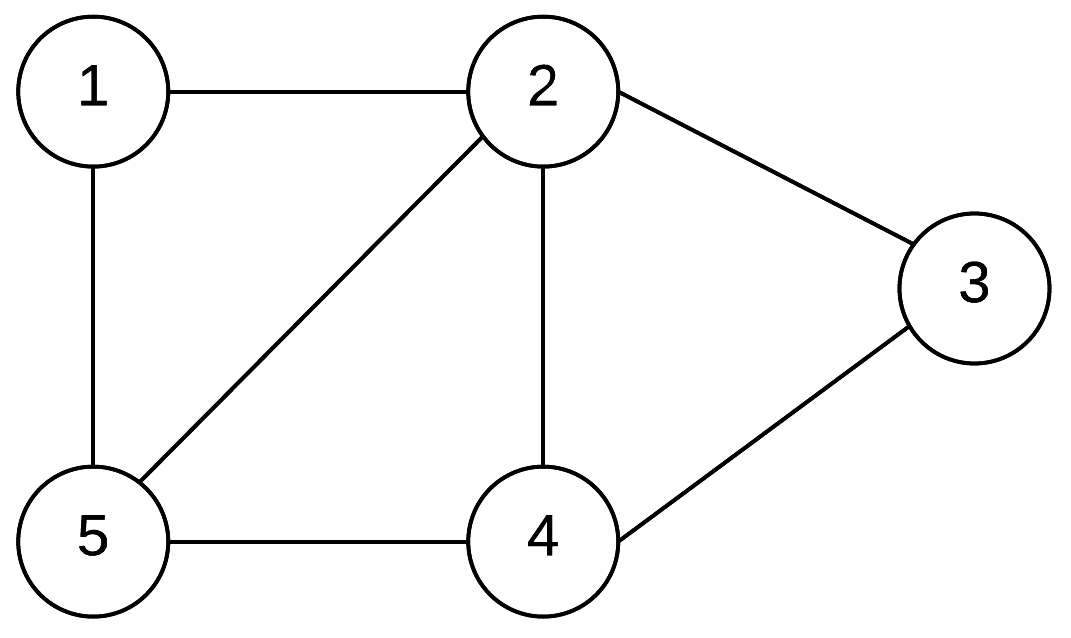
\includegraphics[width=6cm]{defGraph1}
\caption{Example undirected graph}
\end{figure}
\FloatBarrier
\subsection{Adjacency Lists}
There exists an array of size $|V|$, and each element in the array points to a list of adjacent elements in the graph to that node. \\
\[Adj[v]=\text{list of all vertices u}:(v,u)\in E\]
\begin{figure}[h]
\centering
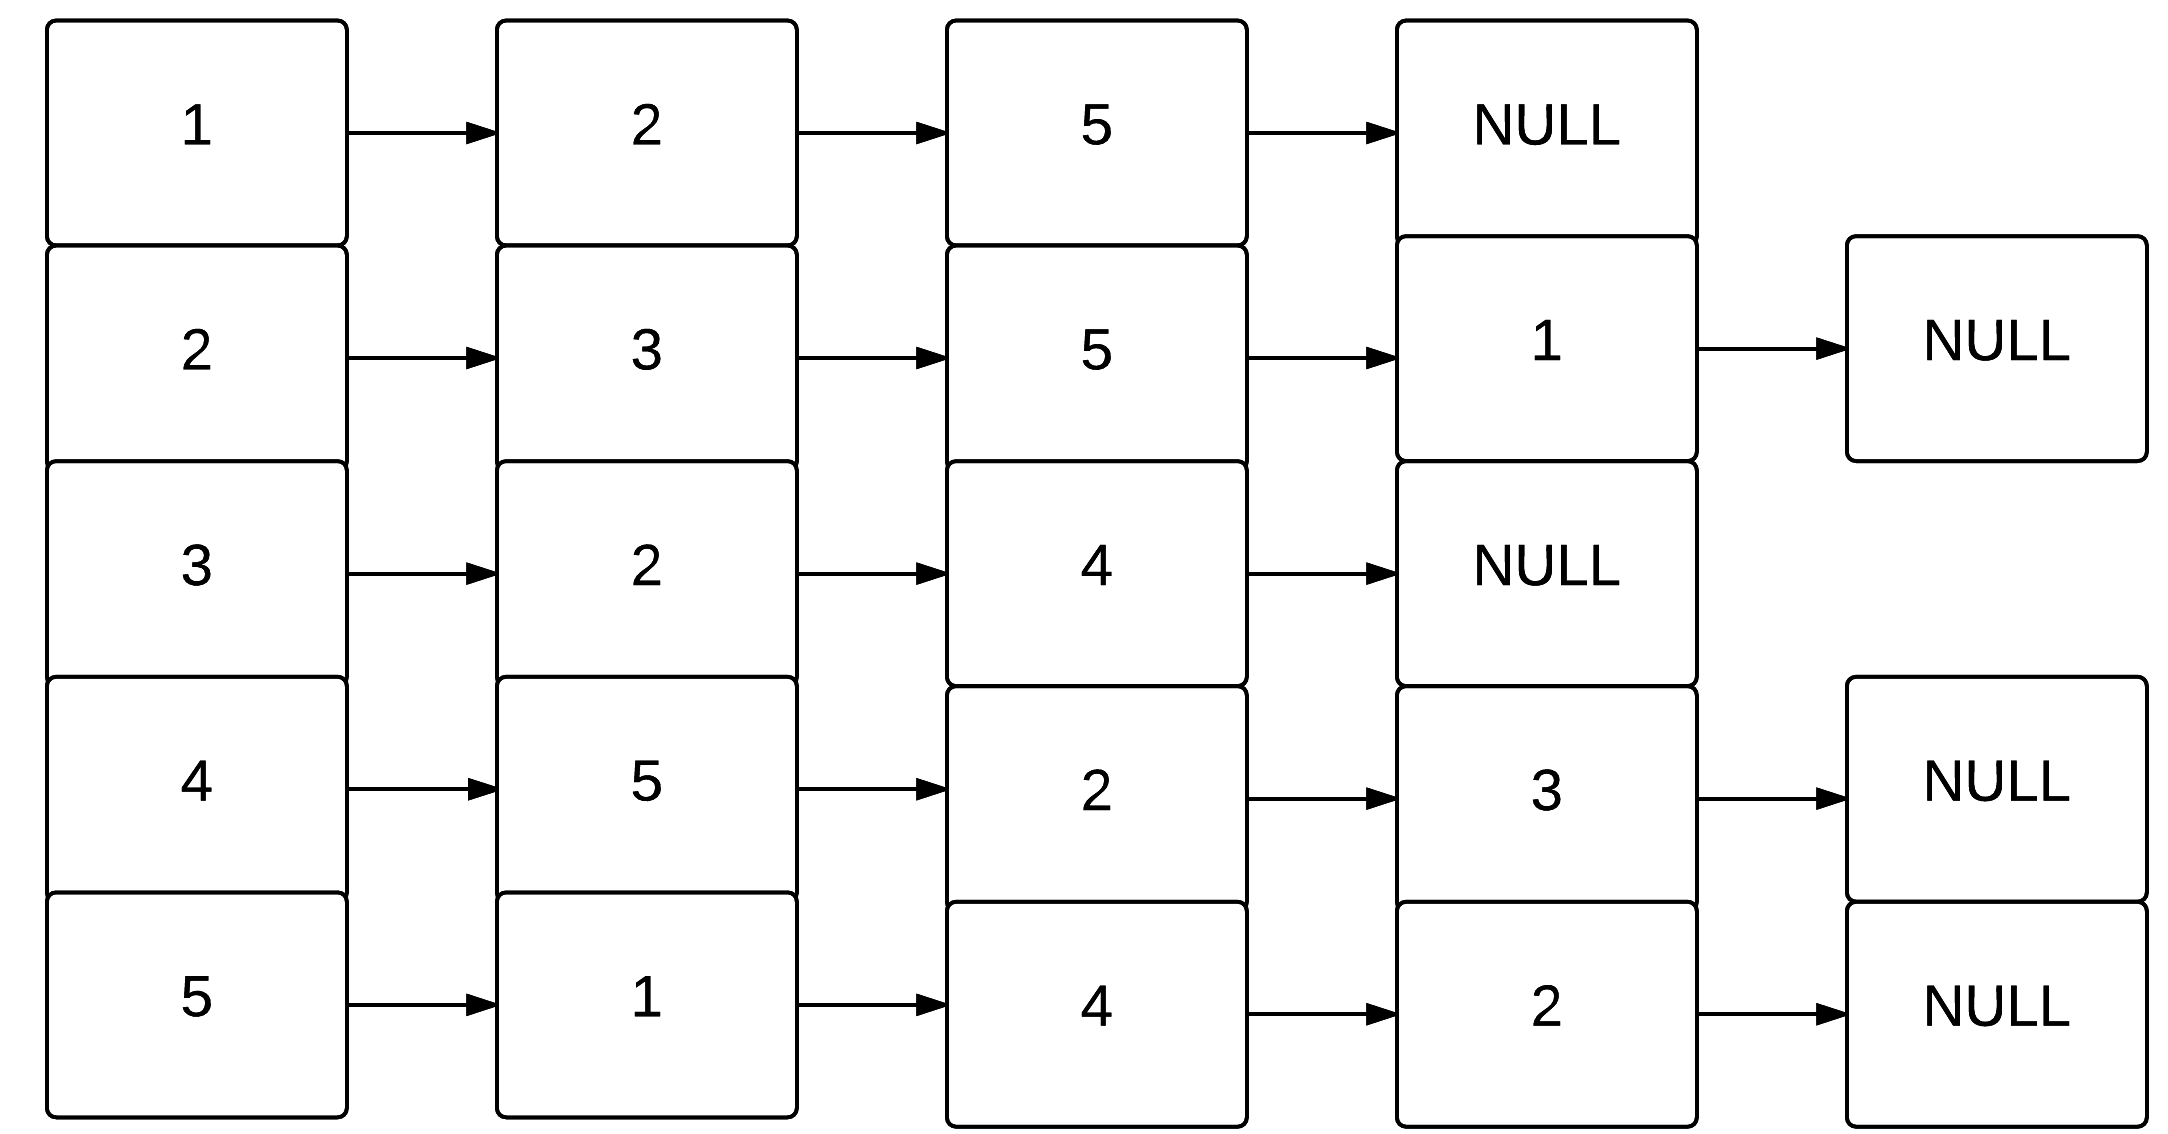
\includegraphics[width=10cm]{AdjList}
\caption{Example of an Adjacency List for the above graph}
\end{figure}
If the graph is directed, there will be $|E|$ elements in the list. If the graph is undirected, there will be $2|E|$ elements in the list. The memory complexity is $\Theta(|V|+|E|)$.
\subsection{Adjacency Matrix}
Matrix $M=|V|\times |V|$\\
\[M[i,j]=\begin{cases}1 & (i,j)\in E \\ 0 & else \end{cases}\]
If the graph is undirected, the resulting associated matrix is symmetric about the diagonal, which means for all i and j, M[i,j]=M[j,i]. If the graph is directed, this no longer holds. This method has a memory complexity $\Theta(|V|^2)$
\begin{figure}
\centering
\begin{tabular}{|c|c|c|c|c|c|}
\hline
 &1&2&3&4&5\\ \hline
1&0&1&0&0&1 \\ \hline
2&1&0&1&1&1\\ \hline
3&0&1&0&1&0\\ \hline
4&0&1&1&0&1\\ \hline
5&1&1&0&1&0\\ \hline
\end{tabular}
\caption{Example of an Adjacency Matrix for the above graph}
\end{figure}
\subsection{Representation comparison}
\begin{figure}[h]
\centering
\begin{tabular}{|c|c|c|}
\hline
 & Adjacency List & Adjacency Matrix\\\hline\hline
Degree of a node & $\Theta(deg(v))$&$\Theta(|V|)$\\\hline
$\exists(u,v)\in E$&$\Theta(deg(v))$&$\Theta(1)$\\\hline
\end{tabular}
\caption{Basic Operations Cost Table}
\end{figure}
\section{Depth First Search - DFS}
Visit a graph
\begin{itemize}
\item The visit goes deeper and deeper in the graph until it can't find any non-visited nodes then it backtracks to visit other nodes. 
\item Keep track of the predecessor of each visited node.
\item If the graph $G_\pi$, induced by the set of predecessors, is considered, then $G_\pi$ is a forest, and, specifically, a DFS forest.
\item Each node will consist of 2 attributes:
\begin{itemize}
\item node.$\pi$ - the predecessor of the node in question
\item node.visited (or node.v) - a boolean variable which is false until the node is visited in the course of algorithm execution.
\end{itemize}
\item The complexity is $\Theta(|V|+\sum_{u\in V}{deg(u)})$ or $\Theta(|V|+|E|)$
\end{itemize}
\subsection{DFS Pseudo code}
\begin{algorithm}
DFS(G) \Begin{
\For{$u\in V$}{
	$u.\pi =$NULL\\
	$u.v=$false\\
}
\For{$u\in V:u.v==false$}{ //for a connected graph this is called once\\
DFSVisit(G,u) \\
}

}
\caption{Depth First Search Pseudo Code}
\label{DFS}
\end{algorithm}
\begin{algorithm}
DFSVisit(G,u) \Begin{
	u.v=true\\
	\For{$v\in Adj(u)$}{
		\If{v.v==false}{
			v.$\pi$=u\\
			DFSVisit(G,v)
		}
	}

}
\caption{Depth First Search Visit Pseudo Code}
\label{DFSVisit}
\end{algorithm}
\FloatBarrier
\subsection{DFS Execution Example}
\begin{figure}[h]
\centering
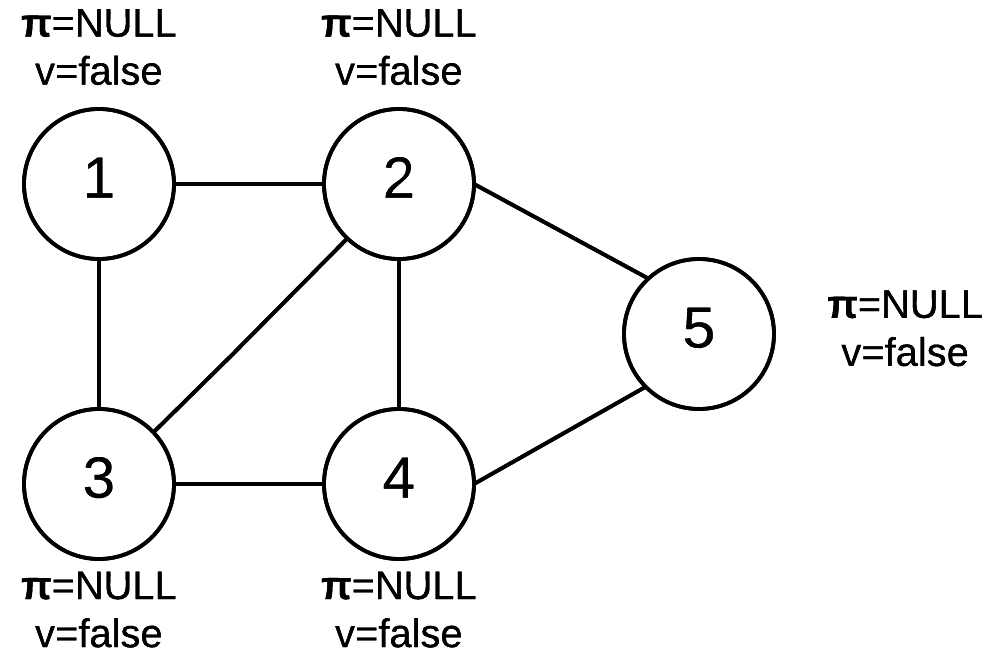
\includegraphics[width=5.5cm]{dfs0}
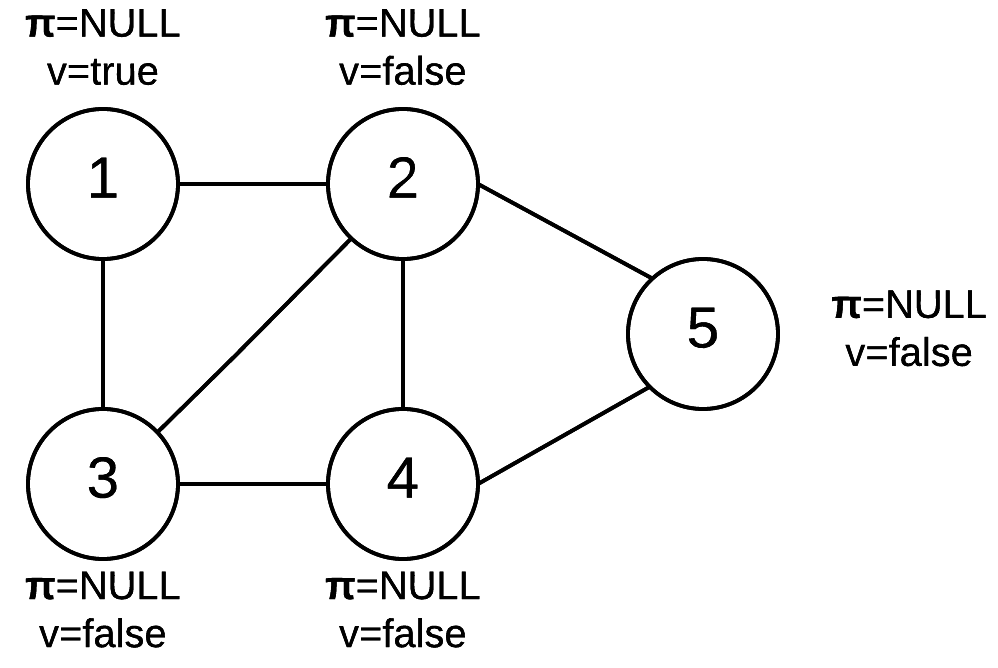
\includegraphics[width=5.5cm]{dfs1}

\end{figure}
\begin{figure}[h]
\centering
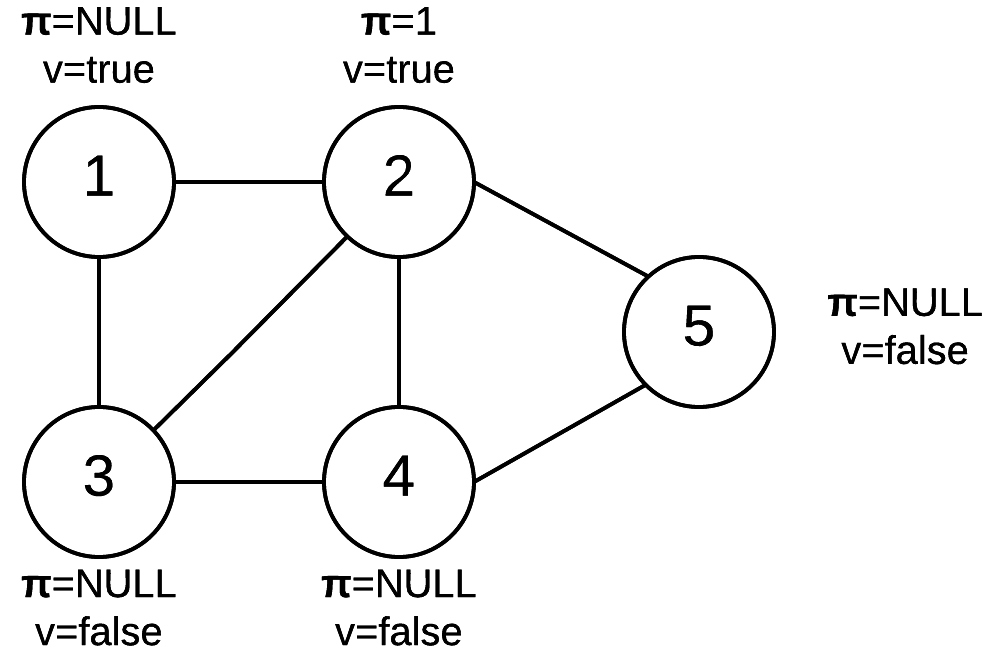
\includegraphics[width=5.5cm]{dfs2}
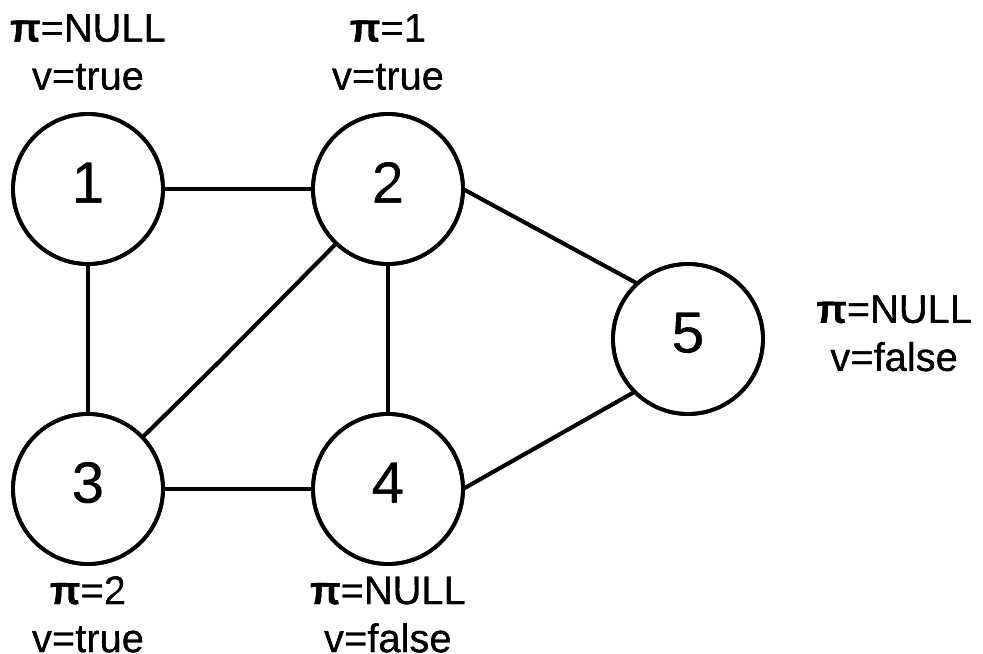
\includegraphics[width=5.5cm]{dfs3}

\end{figure}
\begin{figure}[h]
\centering
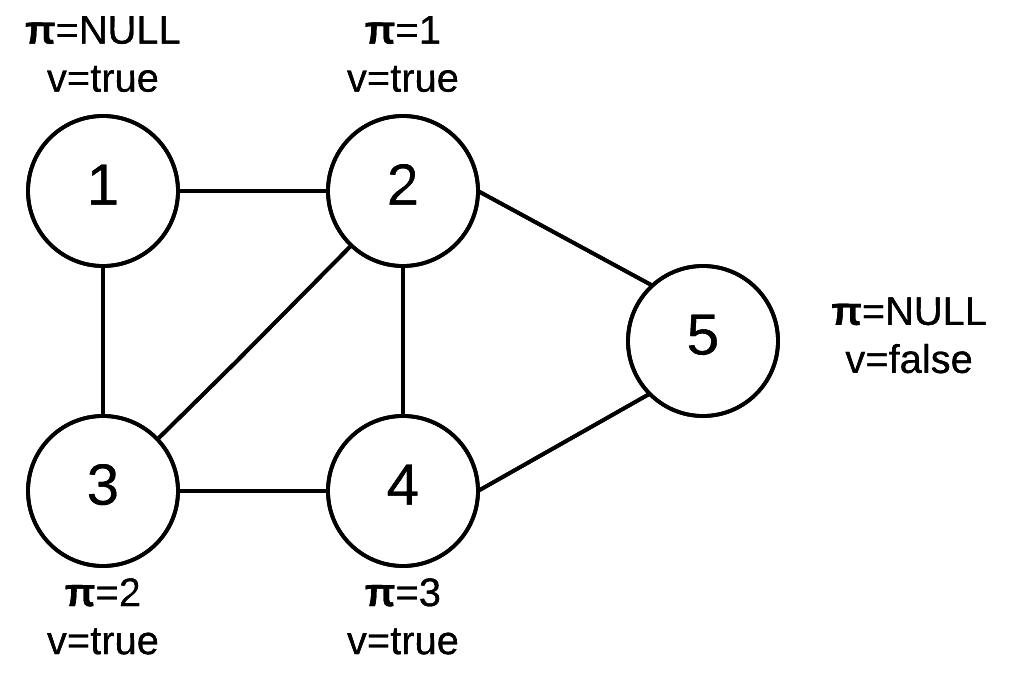
\includegraphics[width=5.5cm]{dfs4}
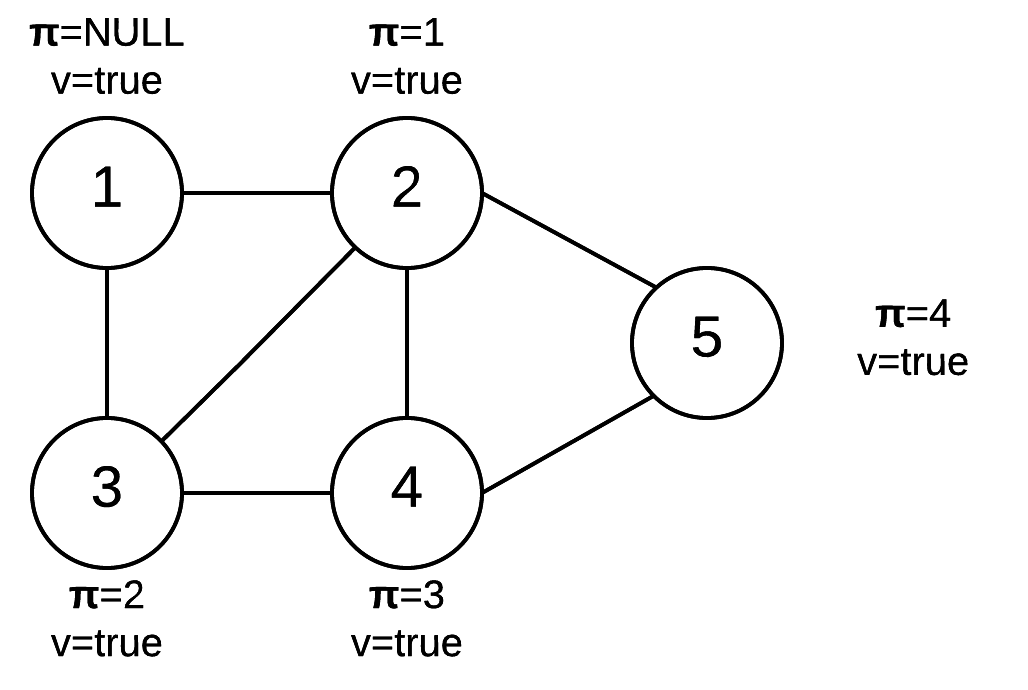
\includegraphics[width=5.5cm]{dfs5}
\caption{Step by step execution of the DFS Algorithm}
\end{figure}
\begin{figure}[h]
\centering
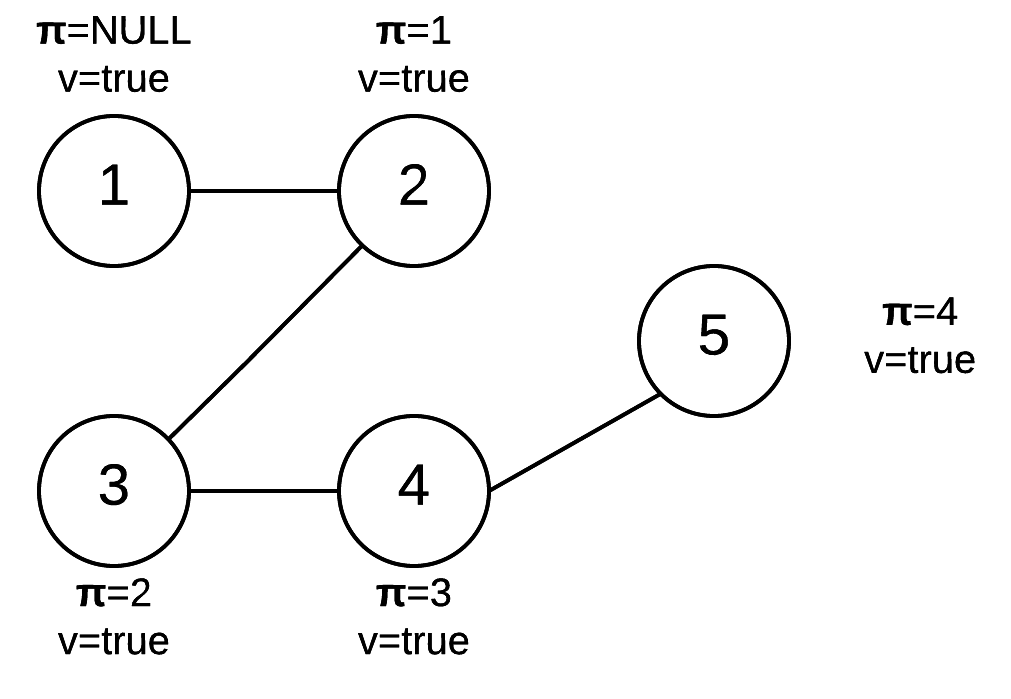
\includegraphics[width=5.5cm]{dfs6g}
\caption{Graph pf the $G_\pi$ Tree}
\end{figure}
\FloatBarrier
\section{Directed Acyclic Graphs (DAG)}
\begin{itemize}
\item Nodes are jobs or activities
\item There exists an edge between u and v (u,v) if v cannot be executed until u has terminated
\item because the graph has no cycles, there must exist at least one activity in degree 0
\item Find a scheduling of activities $v_1',v_2',\dots v_n'$ such that if the activities are executed in the prescribed order, when a general activity is reached, all the activities on which it depends have already been completed 
\end{itemize}
Topological Sorting
\begin{itemize}
\item In the graph representing this, all edges go from left to right. 
\item Topological sorting modifies DFS to add two new attributes 
\begin{itemize}
\item Start (s) - the time at which the visit of $u\in V$ begins.
\item End (e) - the time at which the visit of DFS from u ends. 
\end{itemize}
\item Topological sort is obtained by sorting the nodes in descending order by end time
\end{itemize}
\begin{figure}[h]
\centering
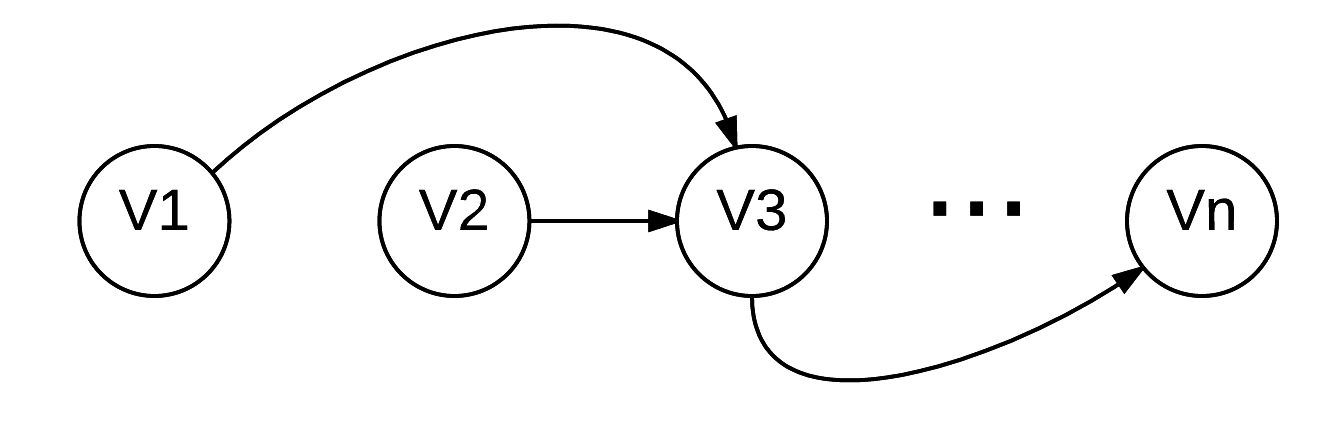
\includegraphics[width=10cm]{Topological}
\end{figure}
\begin{algorithm}
TopologicalDFS(G)\Begin{
	t=0\\
	\For{$u\in V$}{
		u.$\pi$=NULL\\
		u.v=false\\
		u.start=0\\
		u.end=0\\
	}
	\For{$u\in V:u.v==false$}{
		TDFSVisit(G,u)
	}
}
\caption{TopologicalDFS Pseudo Code}
\end{algorithm}
\begin{algorithm}
TDFSVisit(G,u)\Begin{
	t=t+1\\
	u.start=t\\
	u.v=true\\
	\For{$v\in adj(u)$}{
		\If{v.v==false}{
			v.$\pi$=u\\
			TDFSVisit(G,v)
		}
	}
	t=t+1\\
	u.end=t
}
\caption{TDFSVisit Pseudo Code}
\end{algorithm}
\begin{algorithm}
TopologicalSort(G)\Begin{
	TopologicalDFS(G)\\
	Sort nodes by decreasing end time
}
\caption{Overview of Topological Sorting Process Pseudo Code}
\end{algorithm}
\begin{figure}
\centering
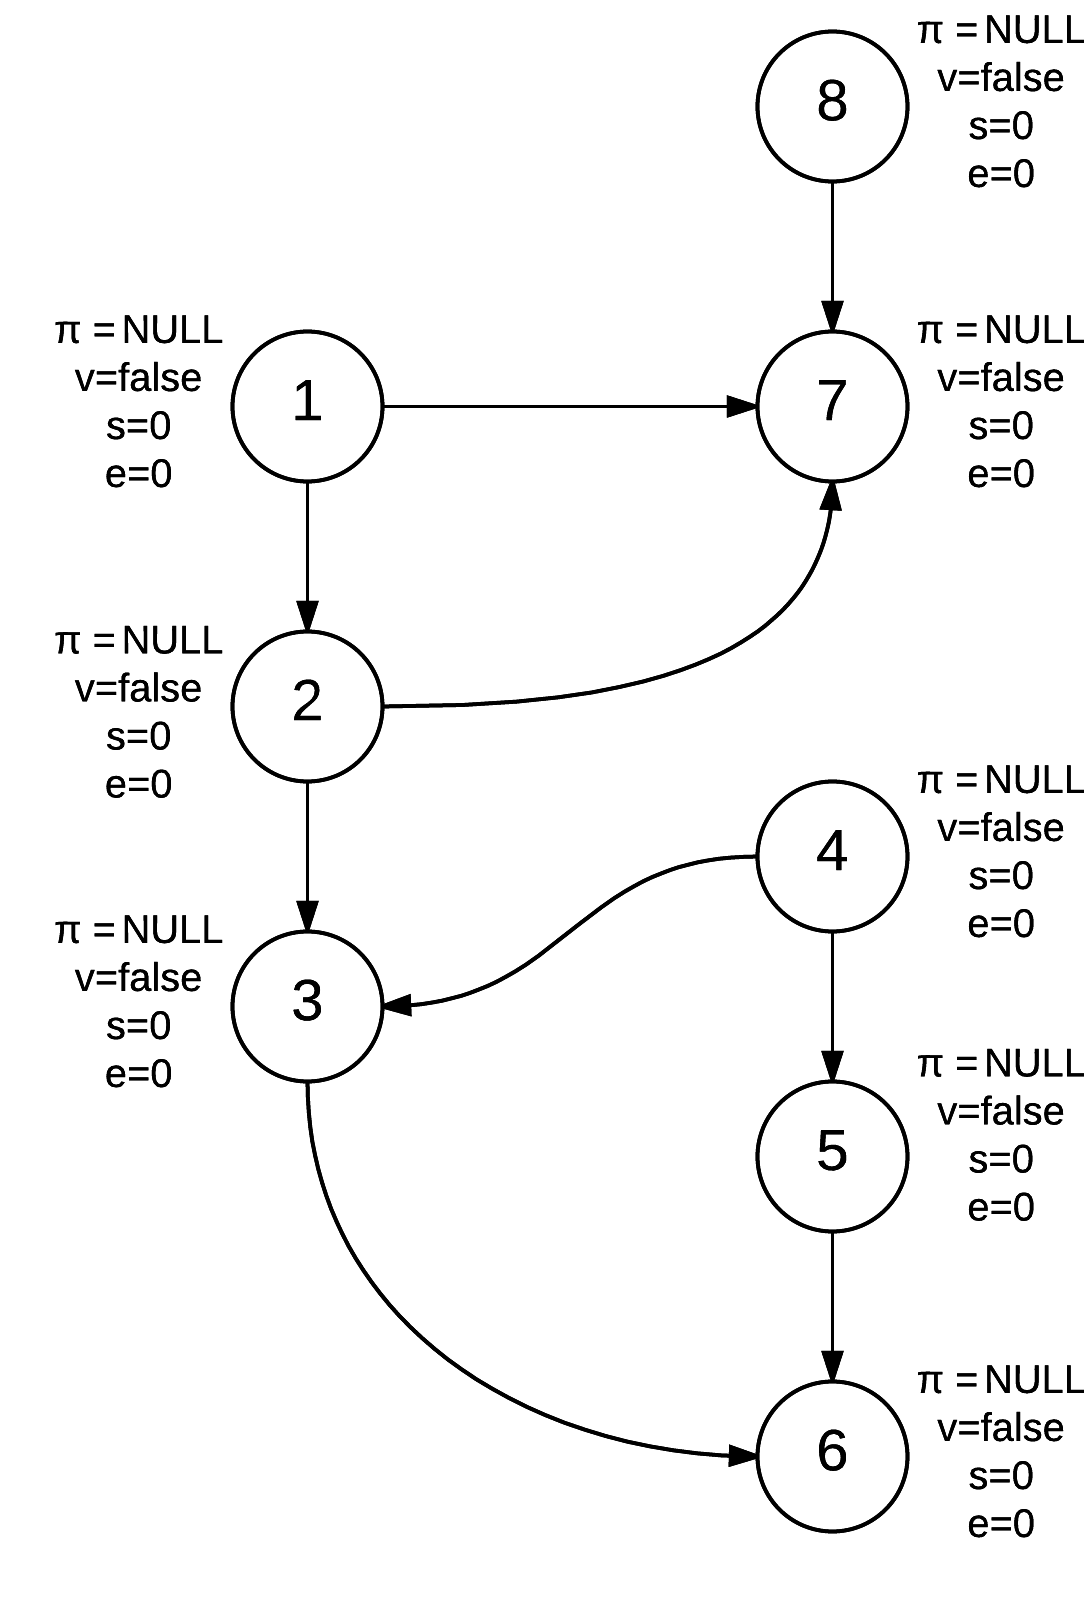
\includegraphics[width=6.5cm]{topo0}
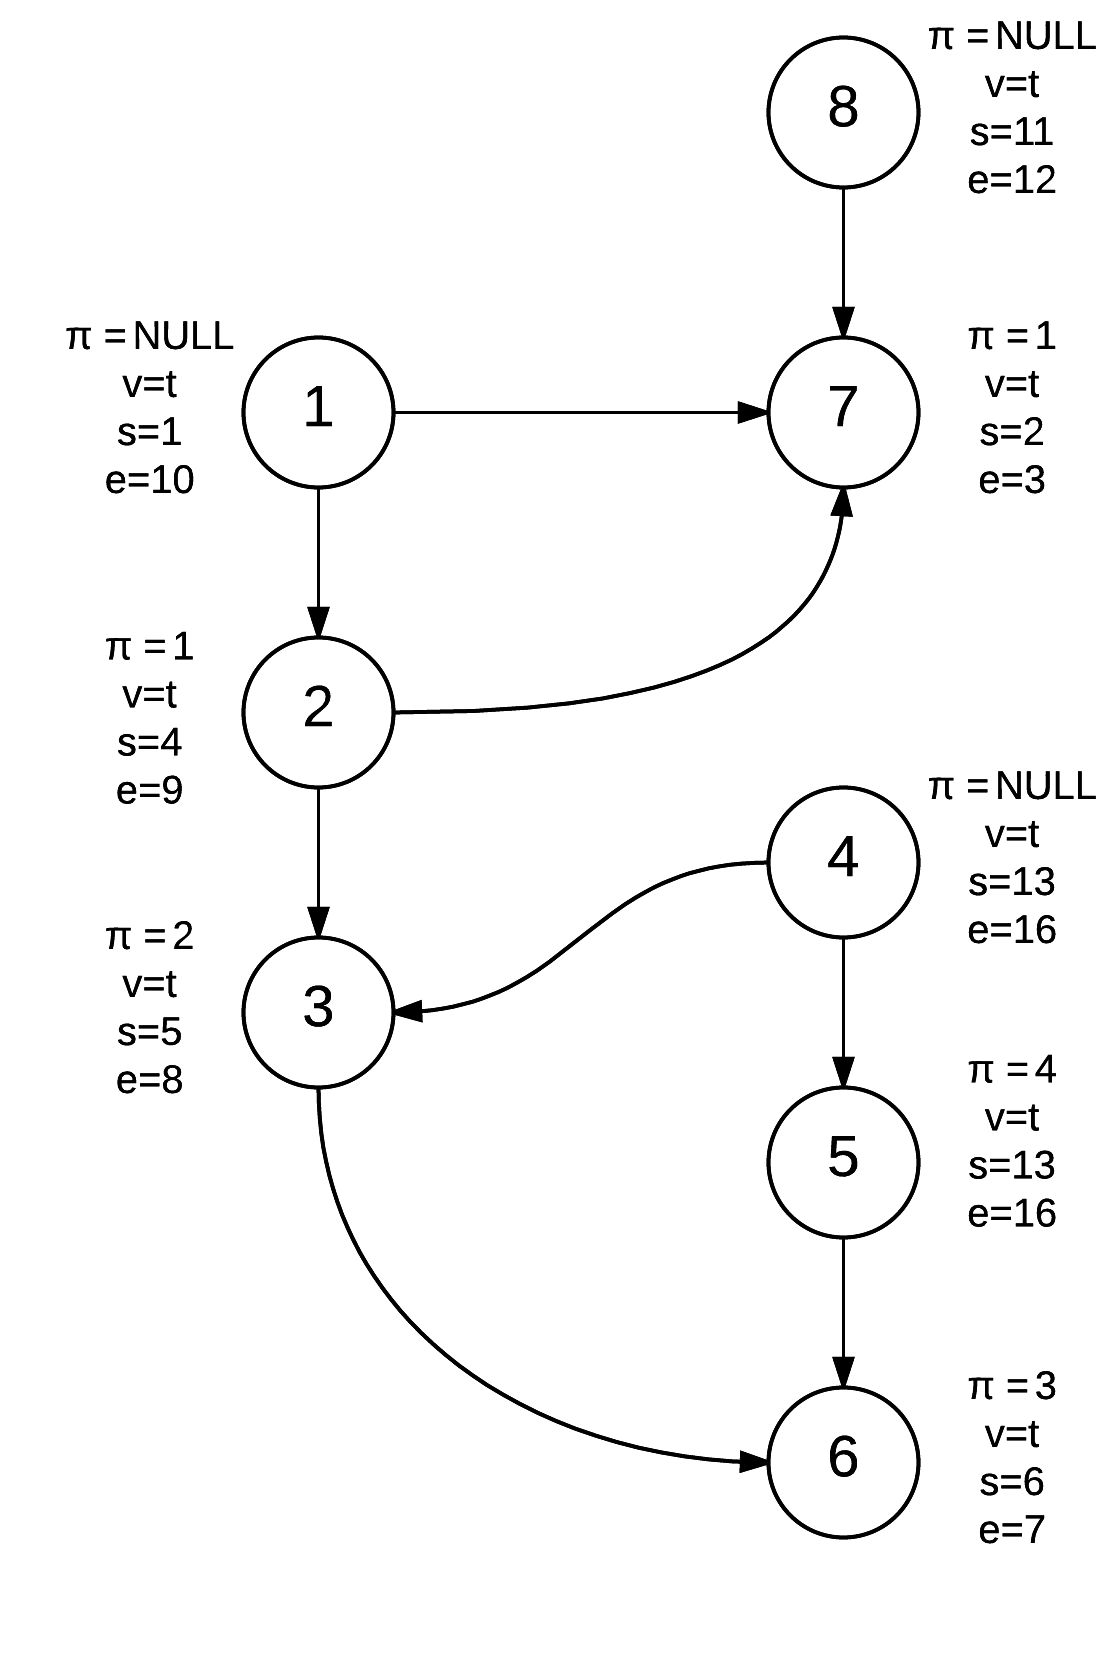
\includegraphics[width=6.5cm]{topofin}
\caption{Initial and final states for the DAG on which the Topological Sorting algorithm is being executed}
\end{figure}
\begin{figure}
\centering
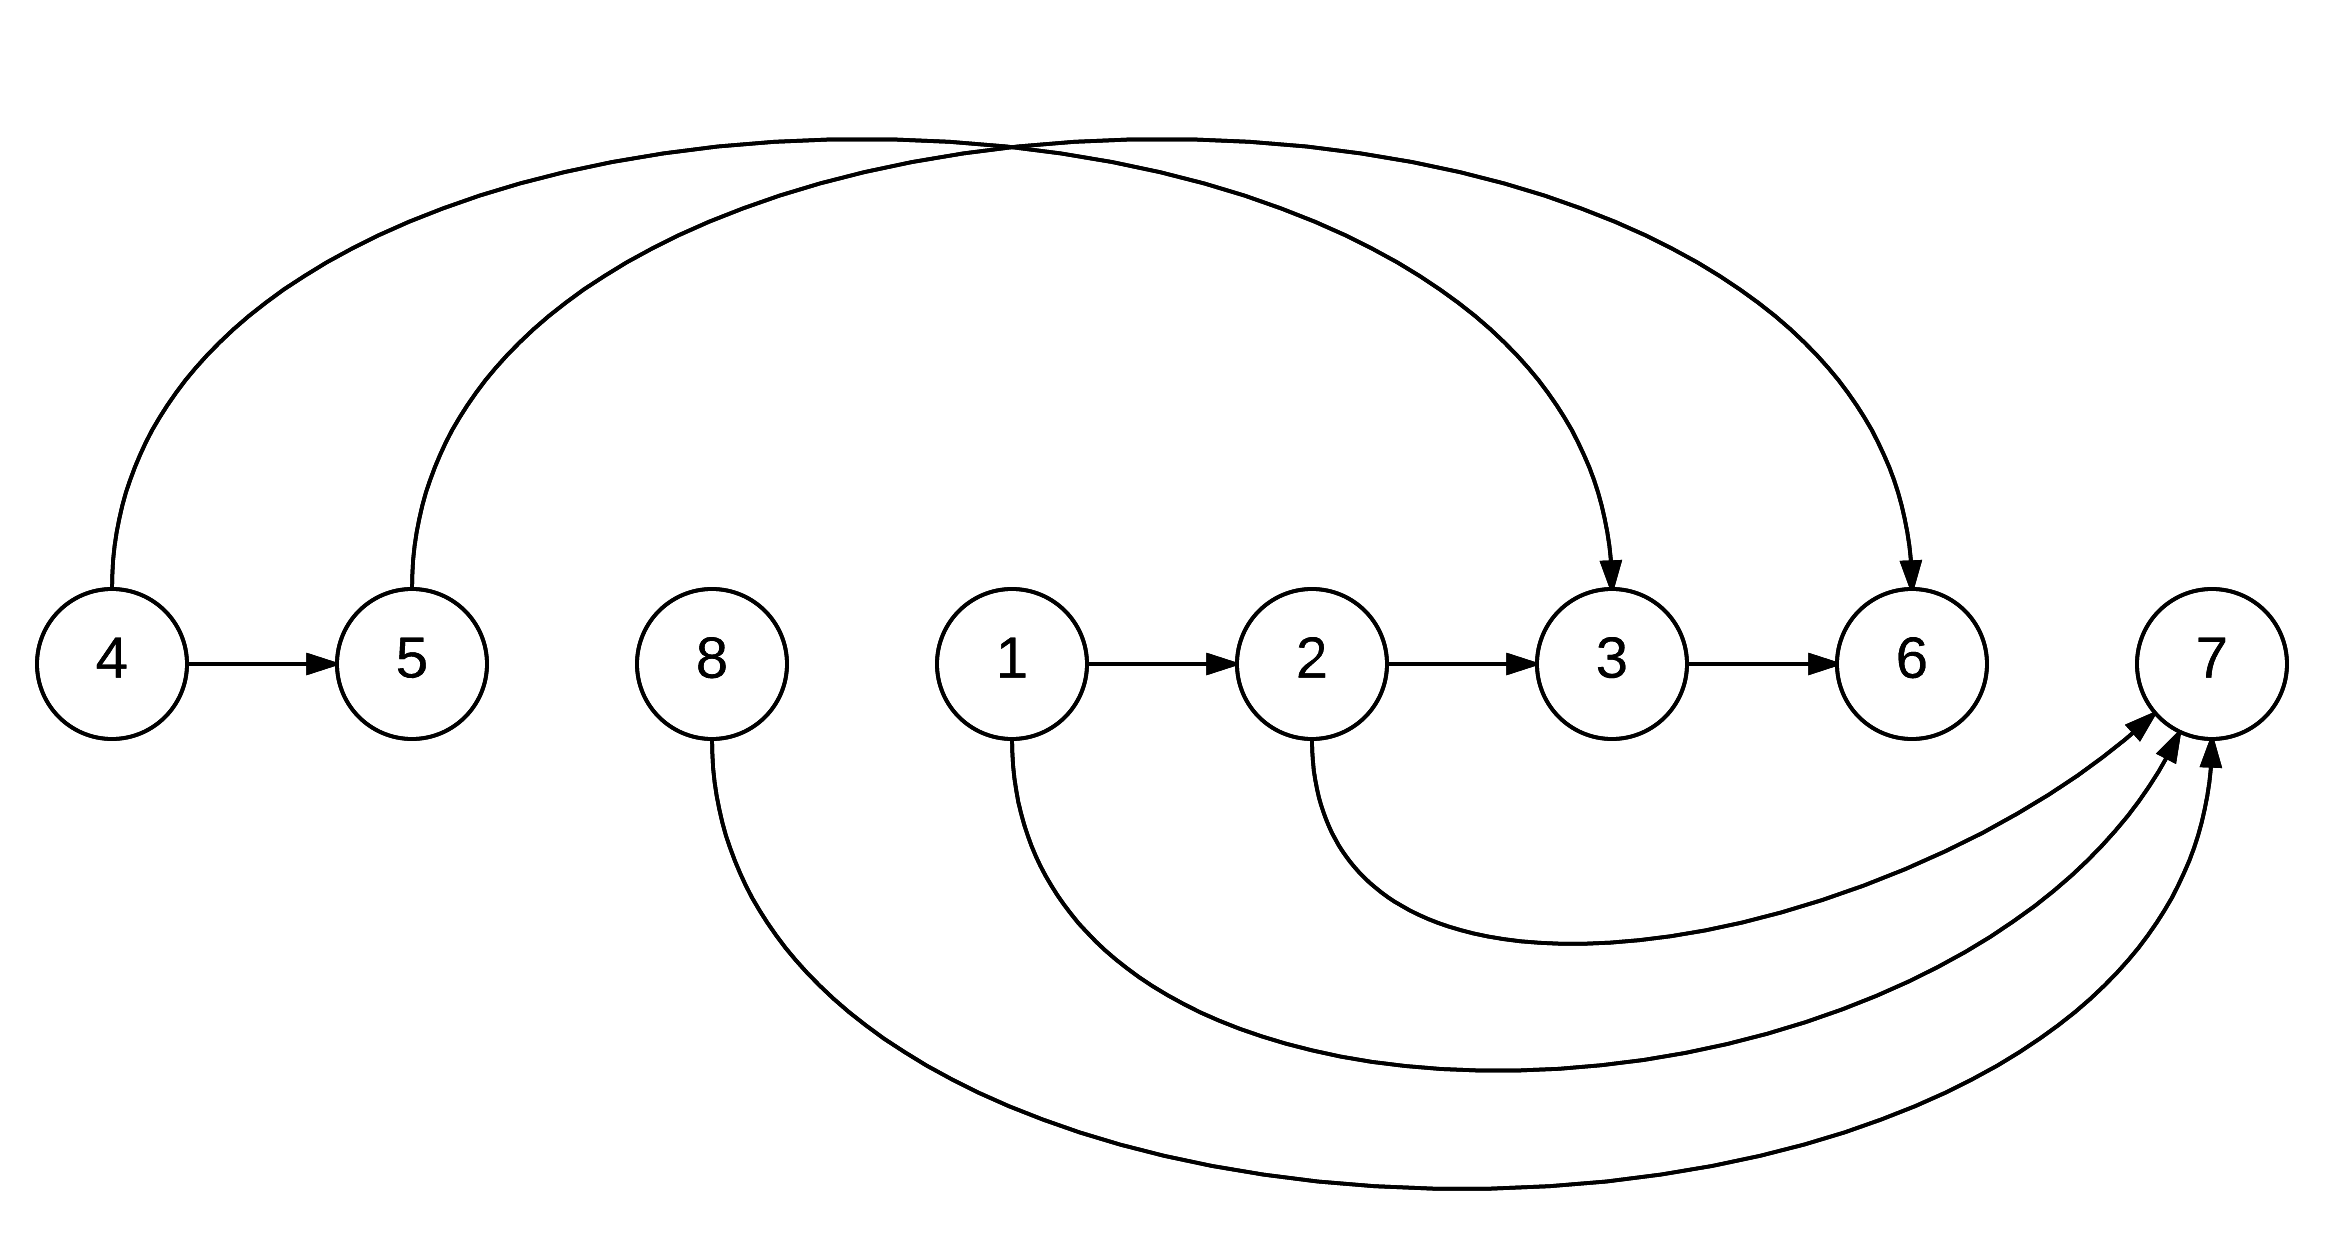
\includegraphics[width=12cm]{TopoSort}
\caption{Final sorted order of the activities according to the Topological Sorting algorithm's execution}
\end{figure}
\FloatBarrier
\section{Breadth First Search (BFS)}
Breadth first search is very similar to depth first search, with the exception that precedence is given to a nodes set of adjacent nodes before going as deep as possible in a graph. Also, one additional attribute is used:
\begin{itemize}
\item u.v, same as previously
\item u.$\pi$, same as previously
\item u.d - the distance from the source to the node in question
\end{itemize}  
Complexity of the Breadth first search: Nodes may be enqueued only once, and the iteration of the internal while loop will happen, at most, $|V|$ times. Enqueue and Dequeue operations are assumed to be constant i.e. $\Theta(1)$, therefore:
\[BFS=\Theta(|V|+\sum_{u\in V}{deg(u))}=\Theta(|V|+|E|)\]
\subsection{BFS Pseudo Code}
\begin{algorithm}
BFS(G,s)\Begin{
	\For{$u\in V \setminus \{s\}$}{
		u.v=false\\
		u.d=$\infty$\\
		u.$\pi$=NULL
	}
	s.v=true\\
	s.d=0\\
	s.$\pi$=NULL\\
	Q=\{\}\\
	Enqueue(Q,s)\\
	\While{$Q\neq\{\}$}{
		u=Dequeue(Q)\\
		\For{$v\in adj(u)$}{
			\If{v.v==false}{
				v.v=true\\
				v.d=u.d+1\\
				v.$\pi$=u\\
				Enqueue(Q,v)
			}
		}
	}
}
\caption{Breadth First Search Pseudocode}
\end{algorithm}
\FloatBarrier
\subsection{BFS Example}
\begin{figure}[h]
\centering
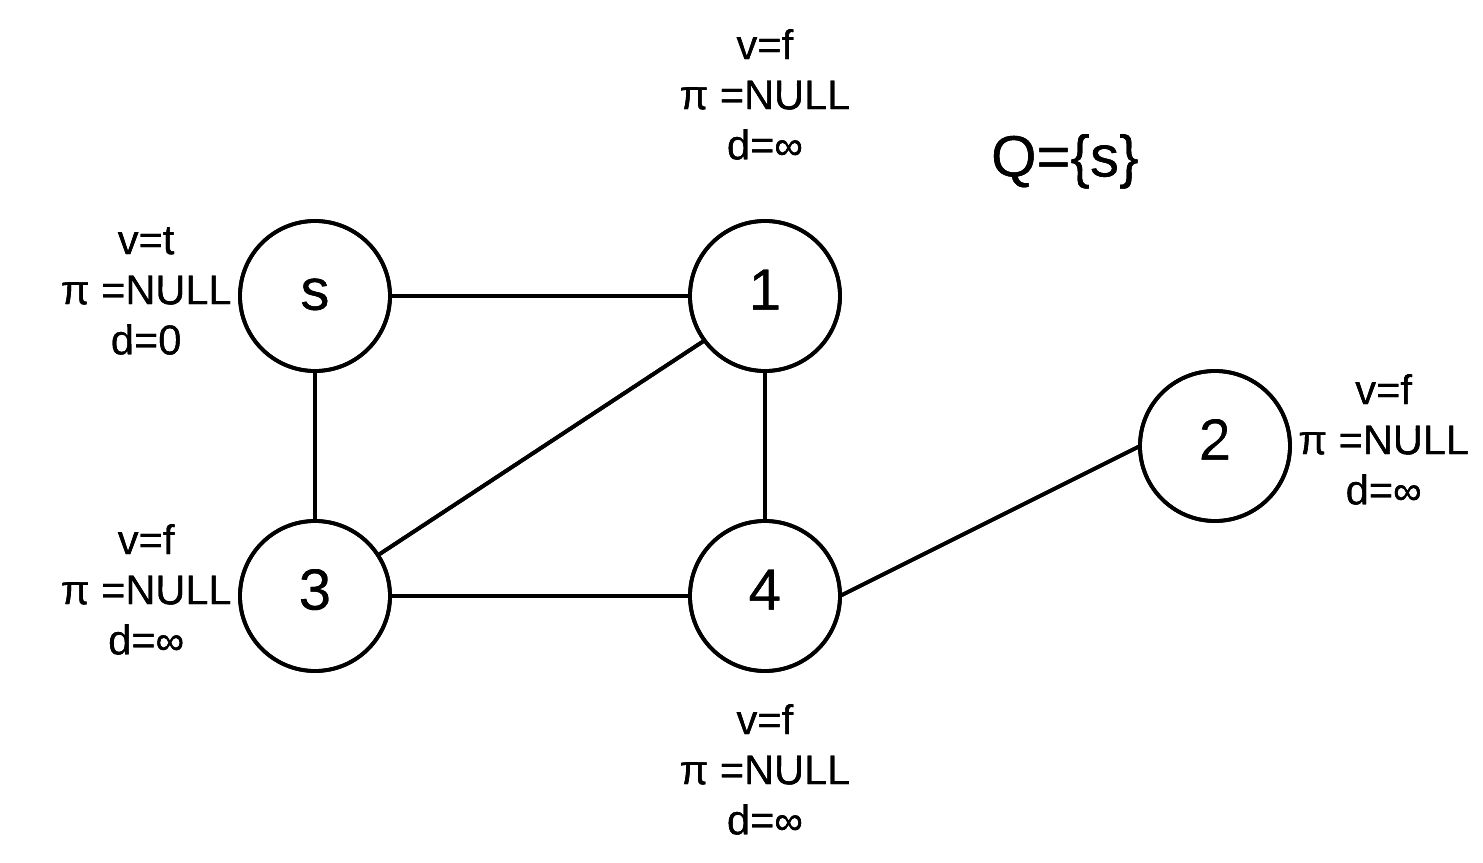
\includegraphics[width=6.5cm]{bfs0}
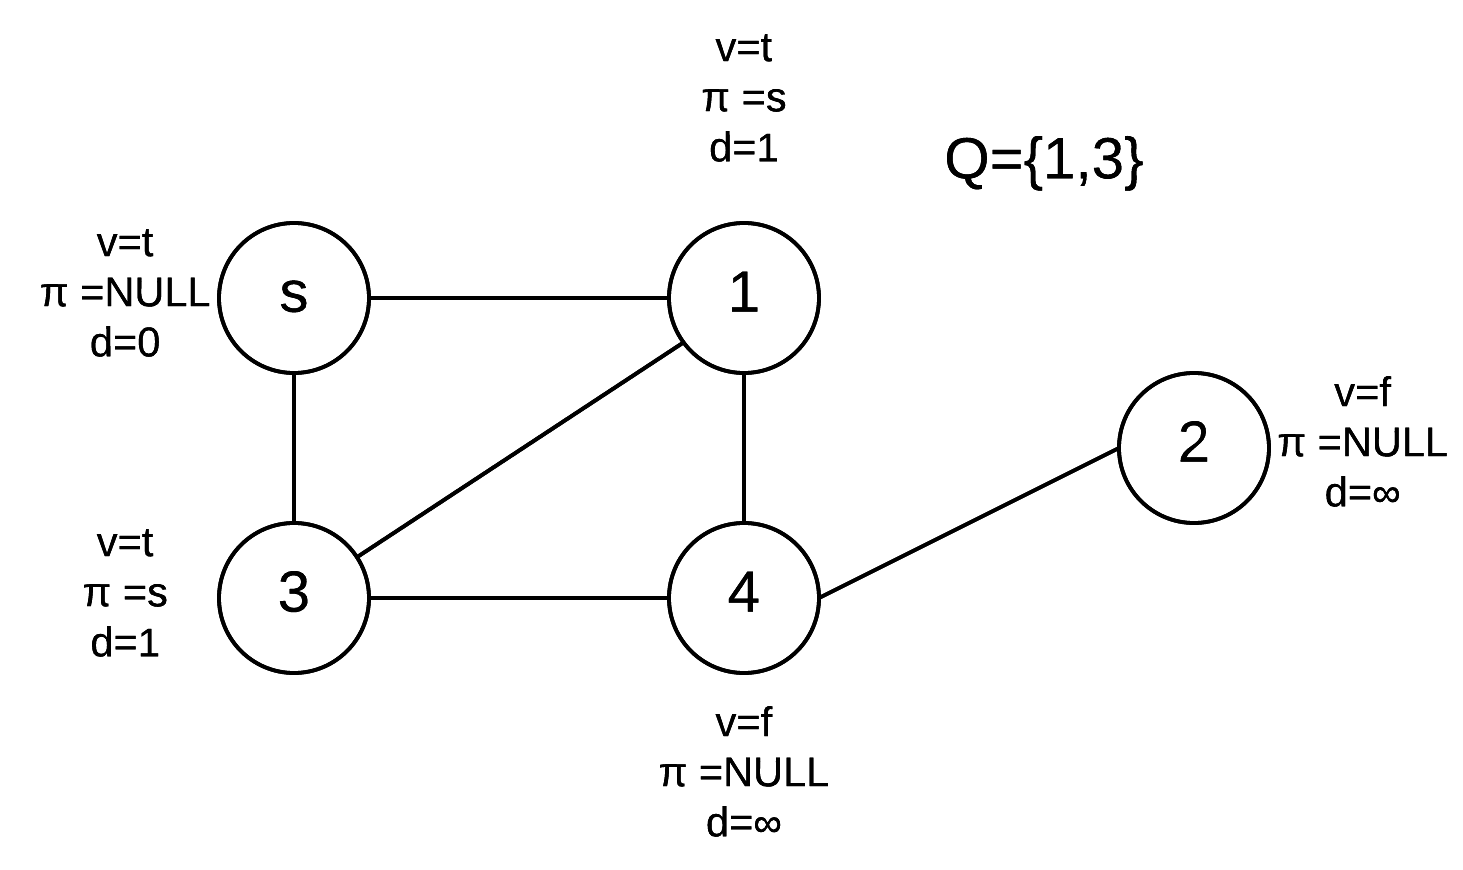
\includegraphics[width=6.5cm]{bfs1}
\end{figure}
\begin{figure}[h]
\centering
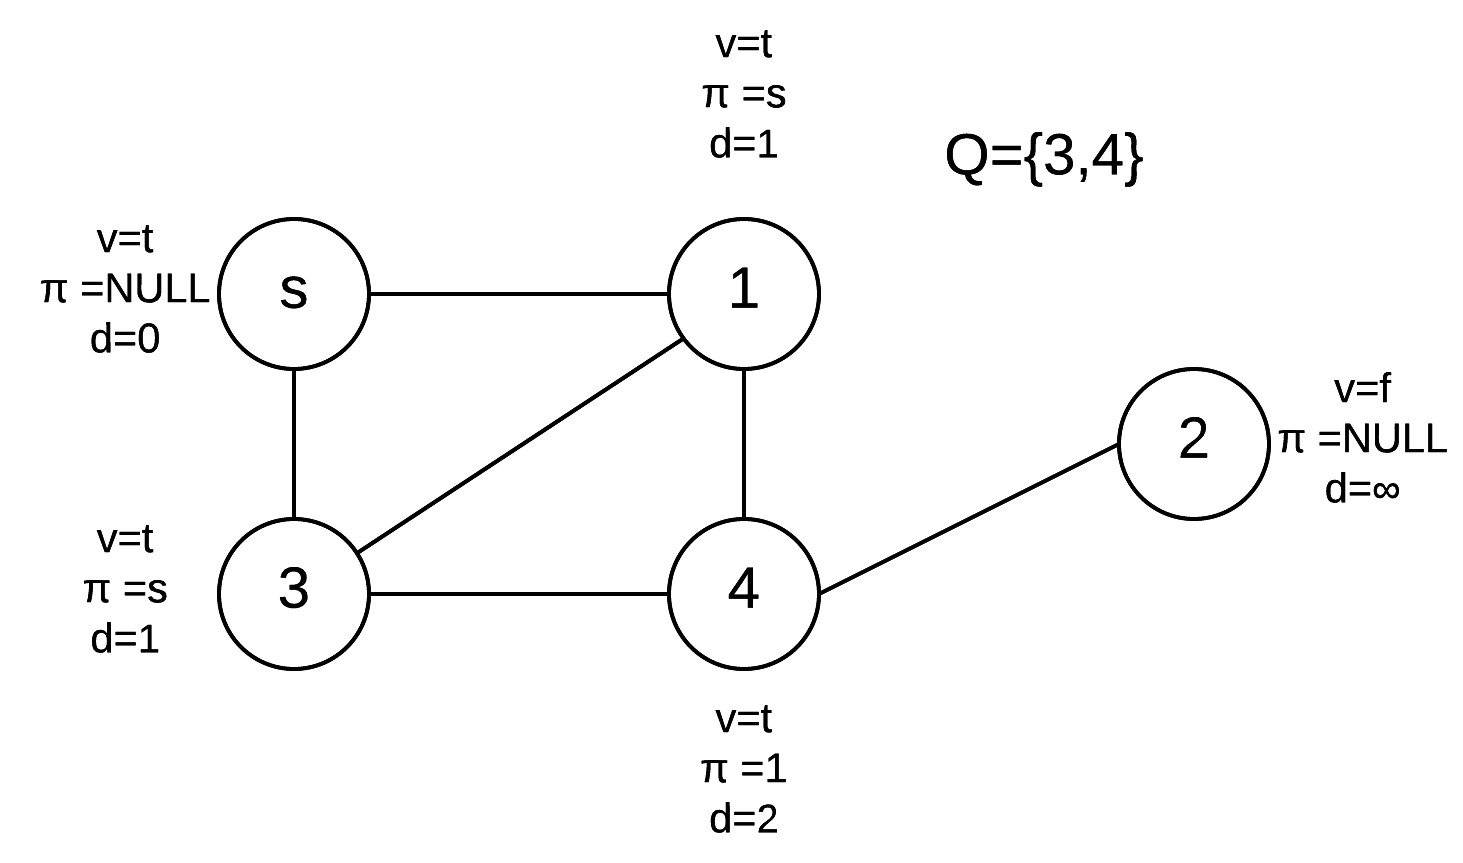
\includegraphics[width=6.5cm]{bfs2}
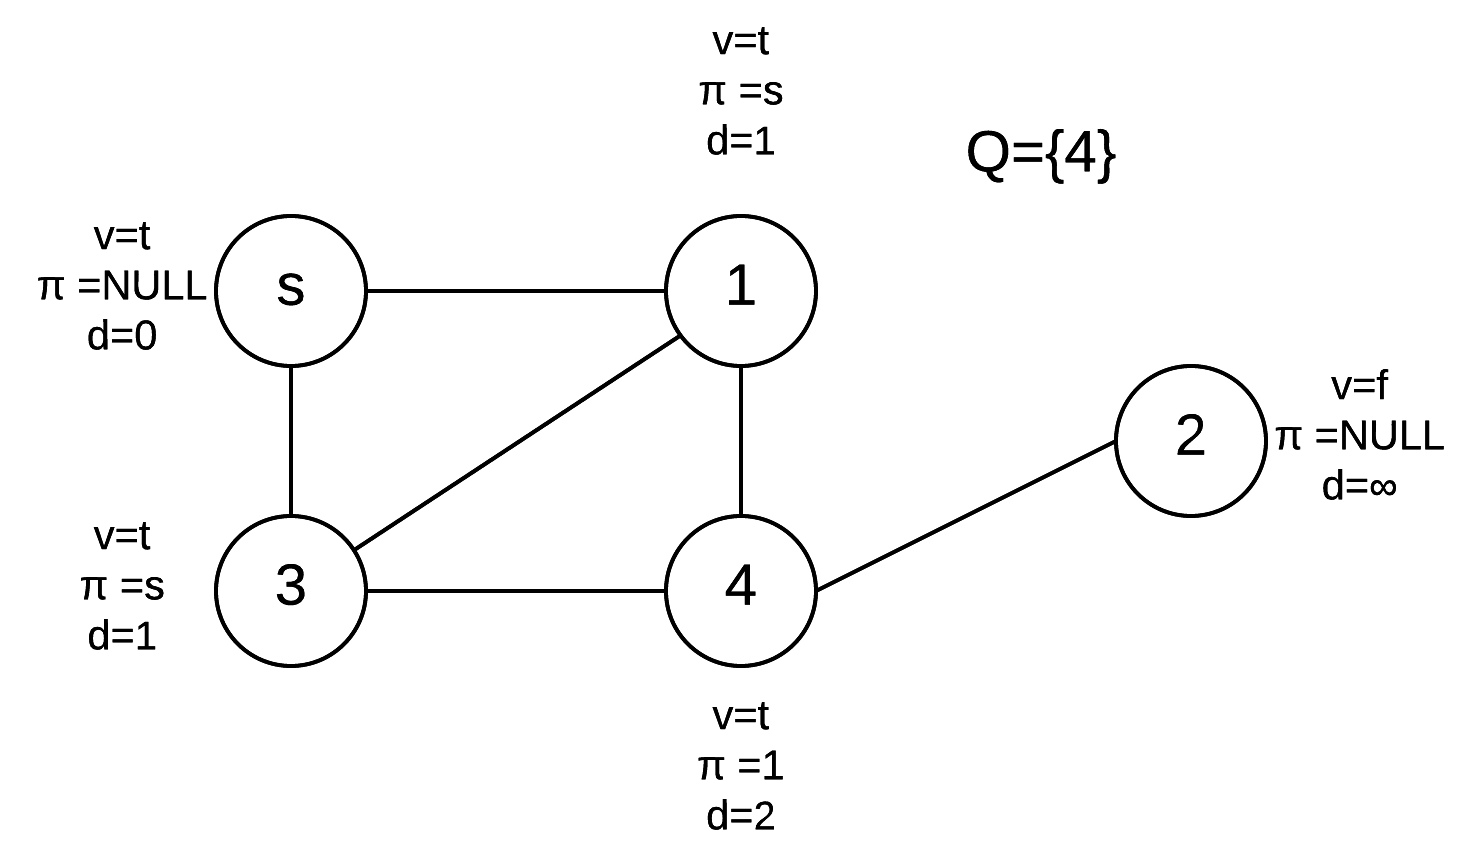
\includegraphics[width=6.5cm]{bfs3}
\end{figure}
\begin{figure}[h]
\centering
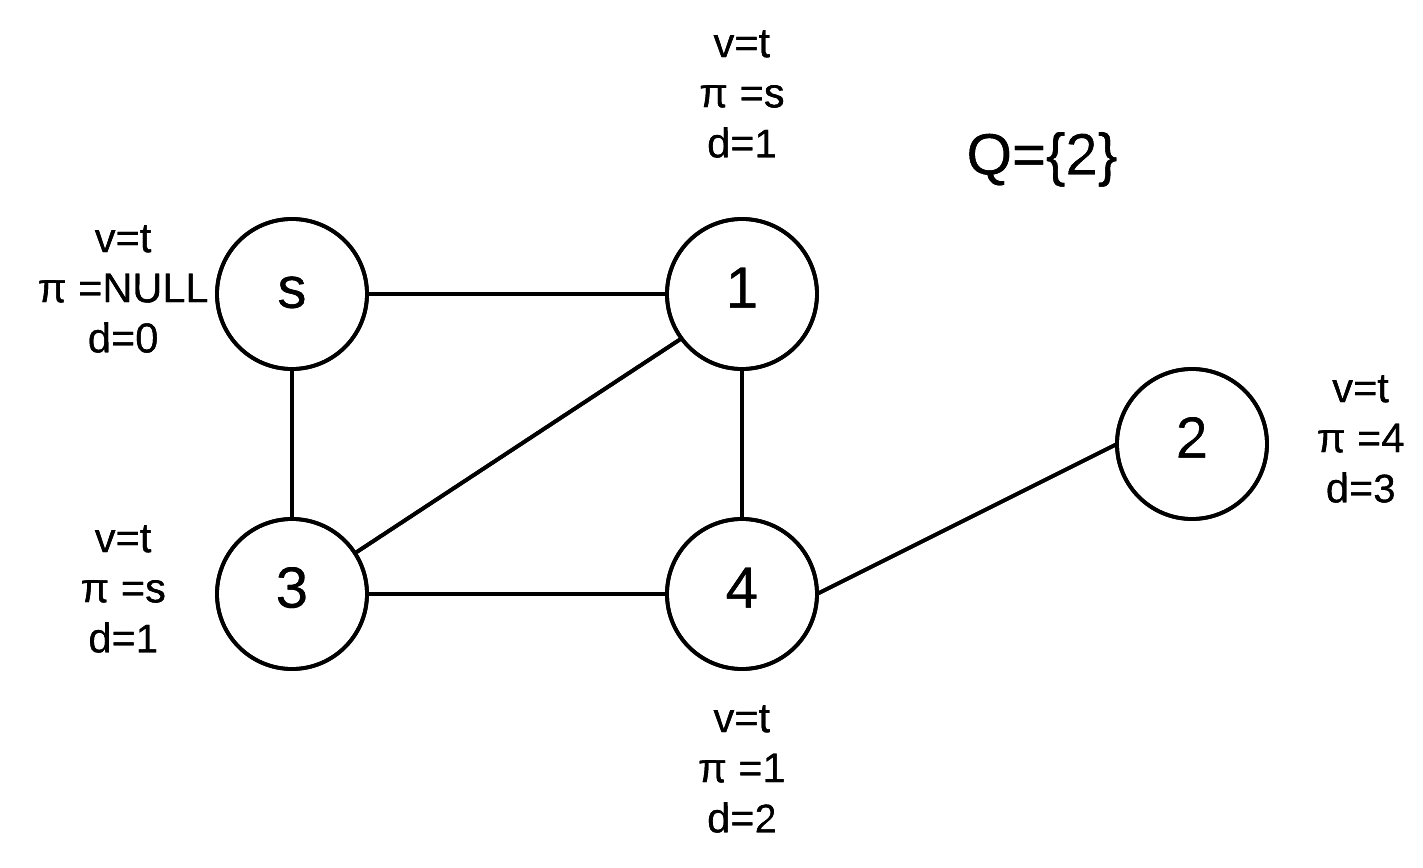
\includegraphics[width=6.5cm]{bfs4}
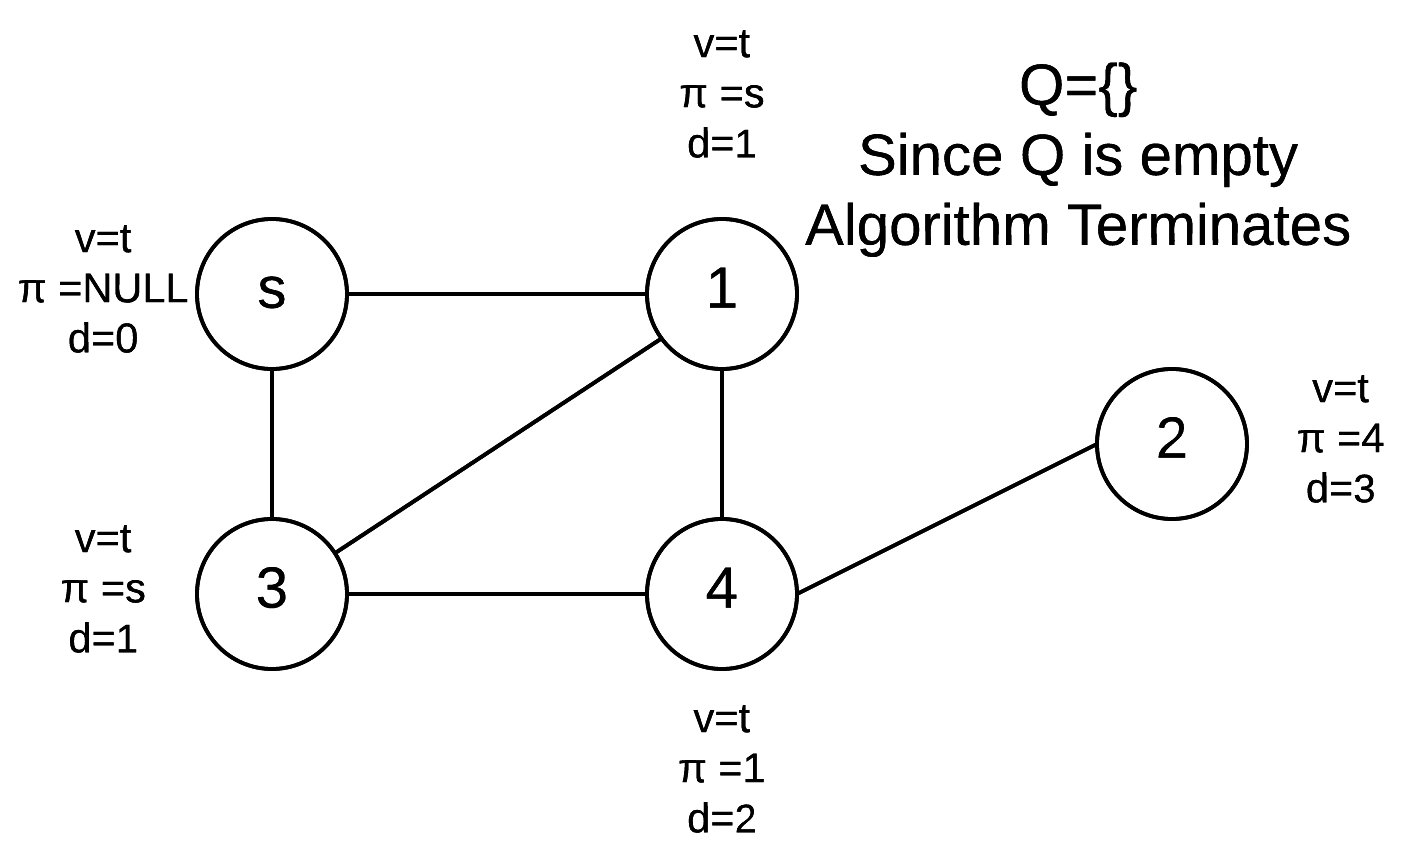
\includegraphics[width=6.5cm]{bfs5}
\caption{Step by step execution of the BFS Algorithm}
\end{figure}
\begin{figure}[h]
\centering
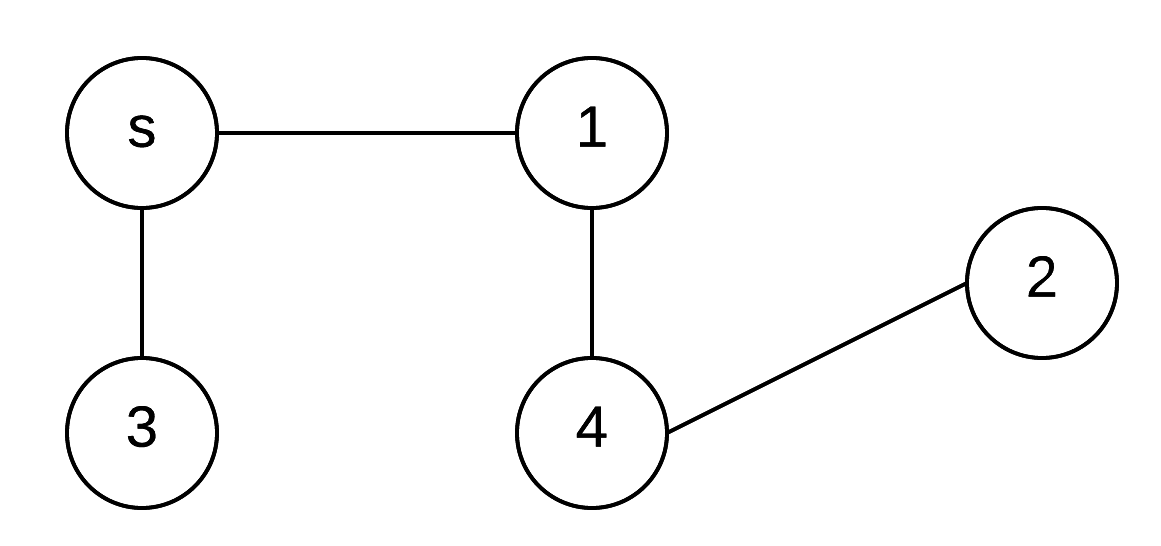
\includegraphics[width=6.5cm]{bfsTree}
\caption{BFS Tree following execution of the algorithm}
\end{figure}
\FloatBarrier
\section{Strongly Connected Components}
\begin{definition}[Strongly Connected Graph]\hfill \break
Directed graphs are strongly connected if, for each pair of nodes, u and v, in V there exists a path from u to v and from v to u. 
\end{definition}
\begin{definition}[Strongly Connected Component]\hfill \break
A strongly connected component c is a subset of V, which is also a subset of the graph, for which the previous definition's property holds, in a manner which describes a maximal subset. 
\end{definition}
\begin{figure}[h]
\centering
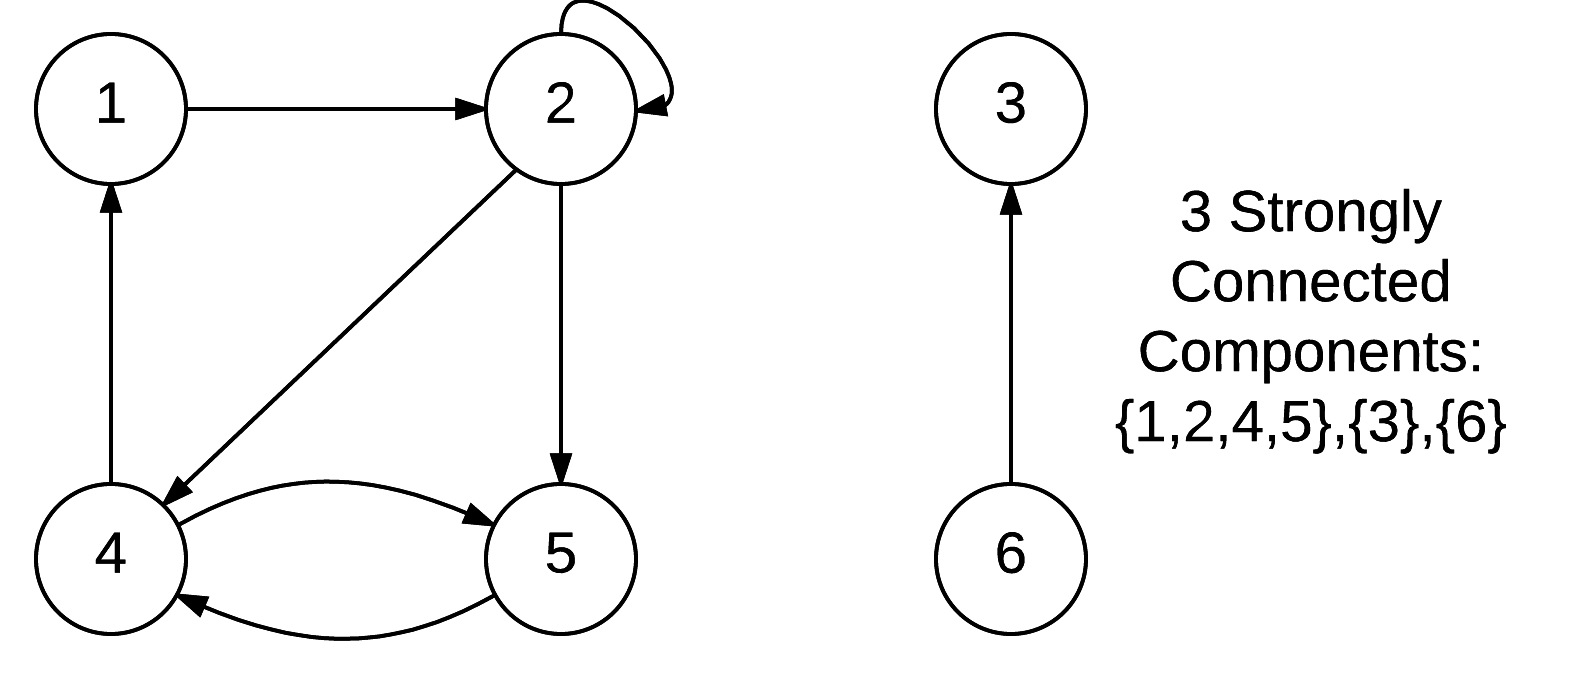
\includegraphics[width=8cm]{sccex}
\caption{Example of a graph and its constituent strongly connected components}
\end{figure}
Given a graph G=(V,E) the transpose $G^T=(V,E^T)$ where $E^T=\{(u,v):(v,u)\in E\}$
\begin{figure}[h]
\centering
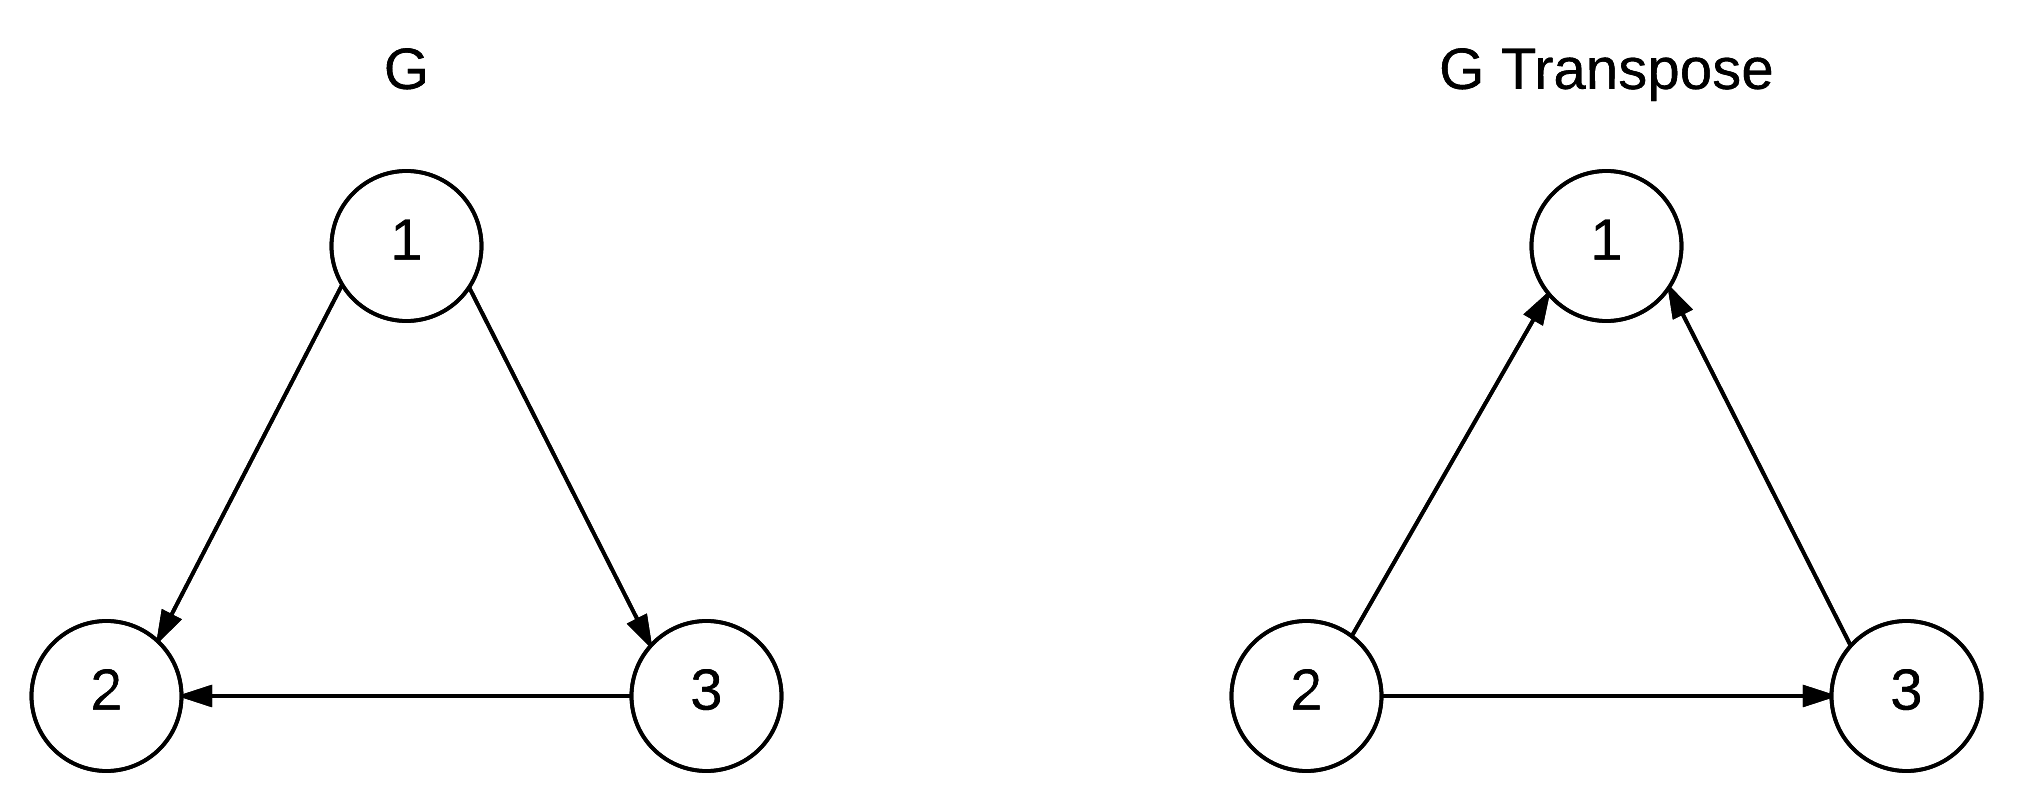
\includegraphics[width=10cm]{graphtranspose}
\end{figure}
\FloatBarrier
In order to find, algorithmically, the strongly connected components of a graph, execute the following steps:
\begin{enumerate}
\item Execute the DFS algorithm while also calculating for all u in V u.e.
\item compute $G^T$.
\item Execute DFS on $G^T$ such that the nodes are considered in decreasing order of finish time computed in step 1.
\item Output each tree in the DFS forest calculated in step 3 as a SCC.
\end{enumerate}
\subsection{SCC Example}
\begin{figure}[h]
\centering
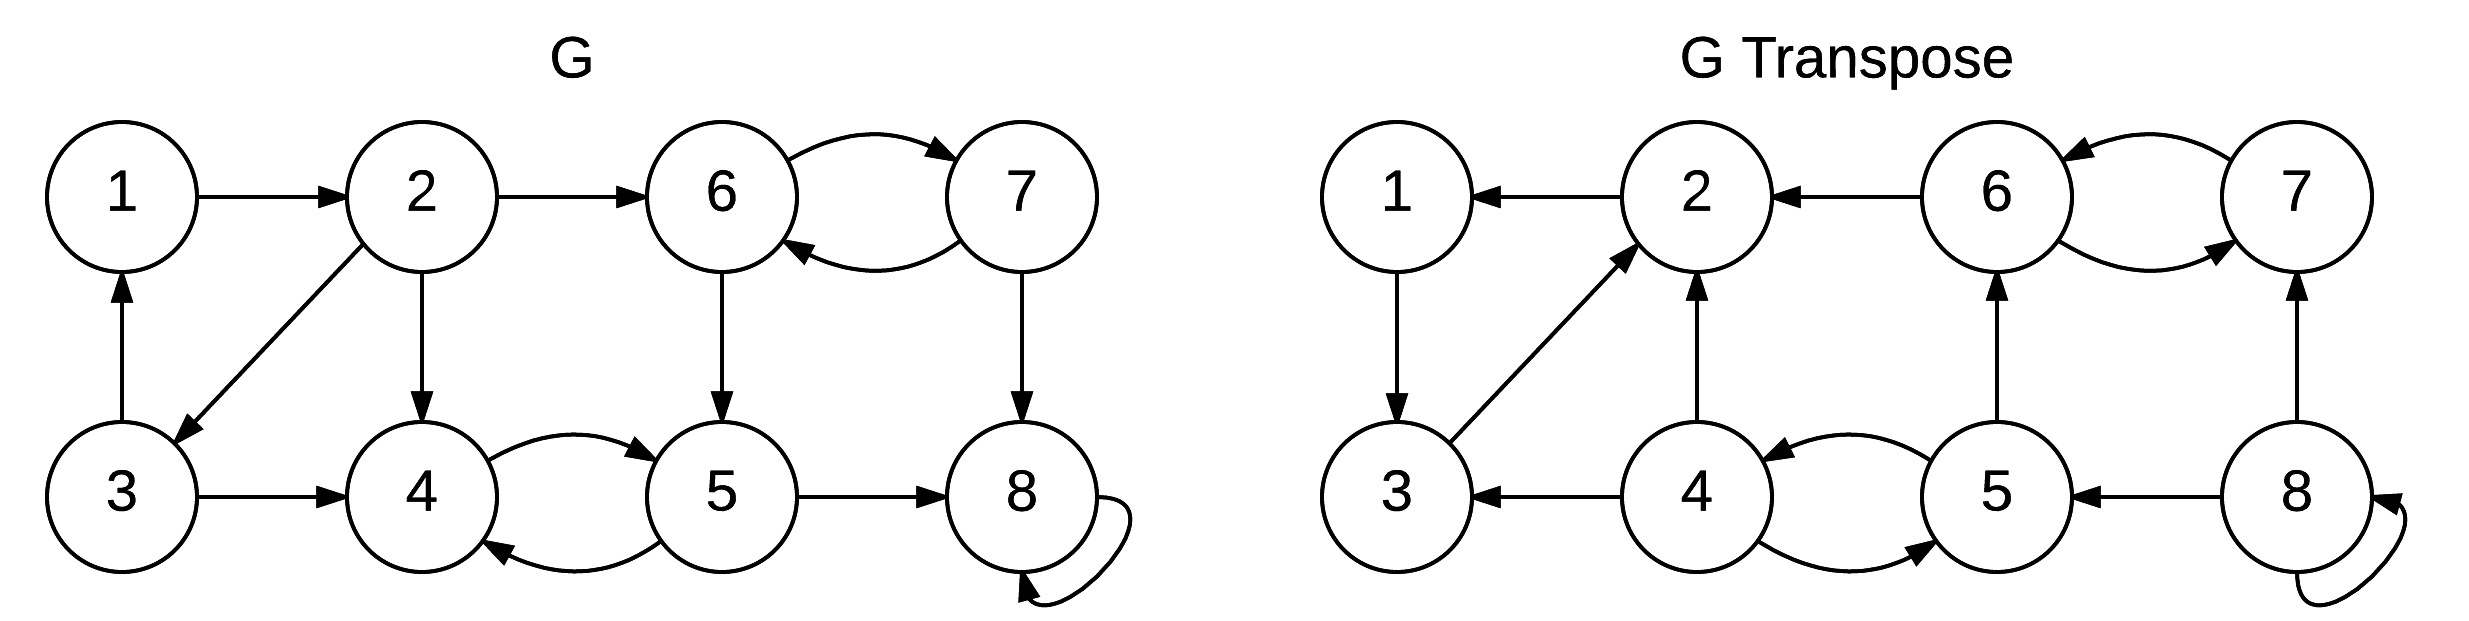
\includegraphics[width=13cm]{scccomplete}
\caption{Graph and its transpose in which the SCCs will be found}
\end{figure}
\begin{enumerate}
\item Execute the DFS algorithm while also calculating for all u in V u.e.
\begin{figure}[h]
\centering
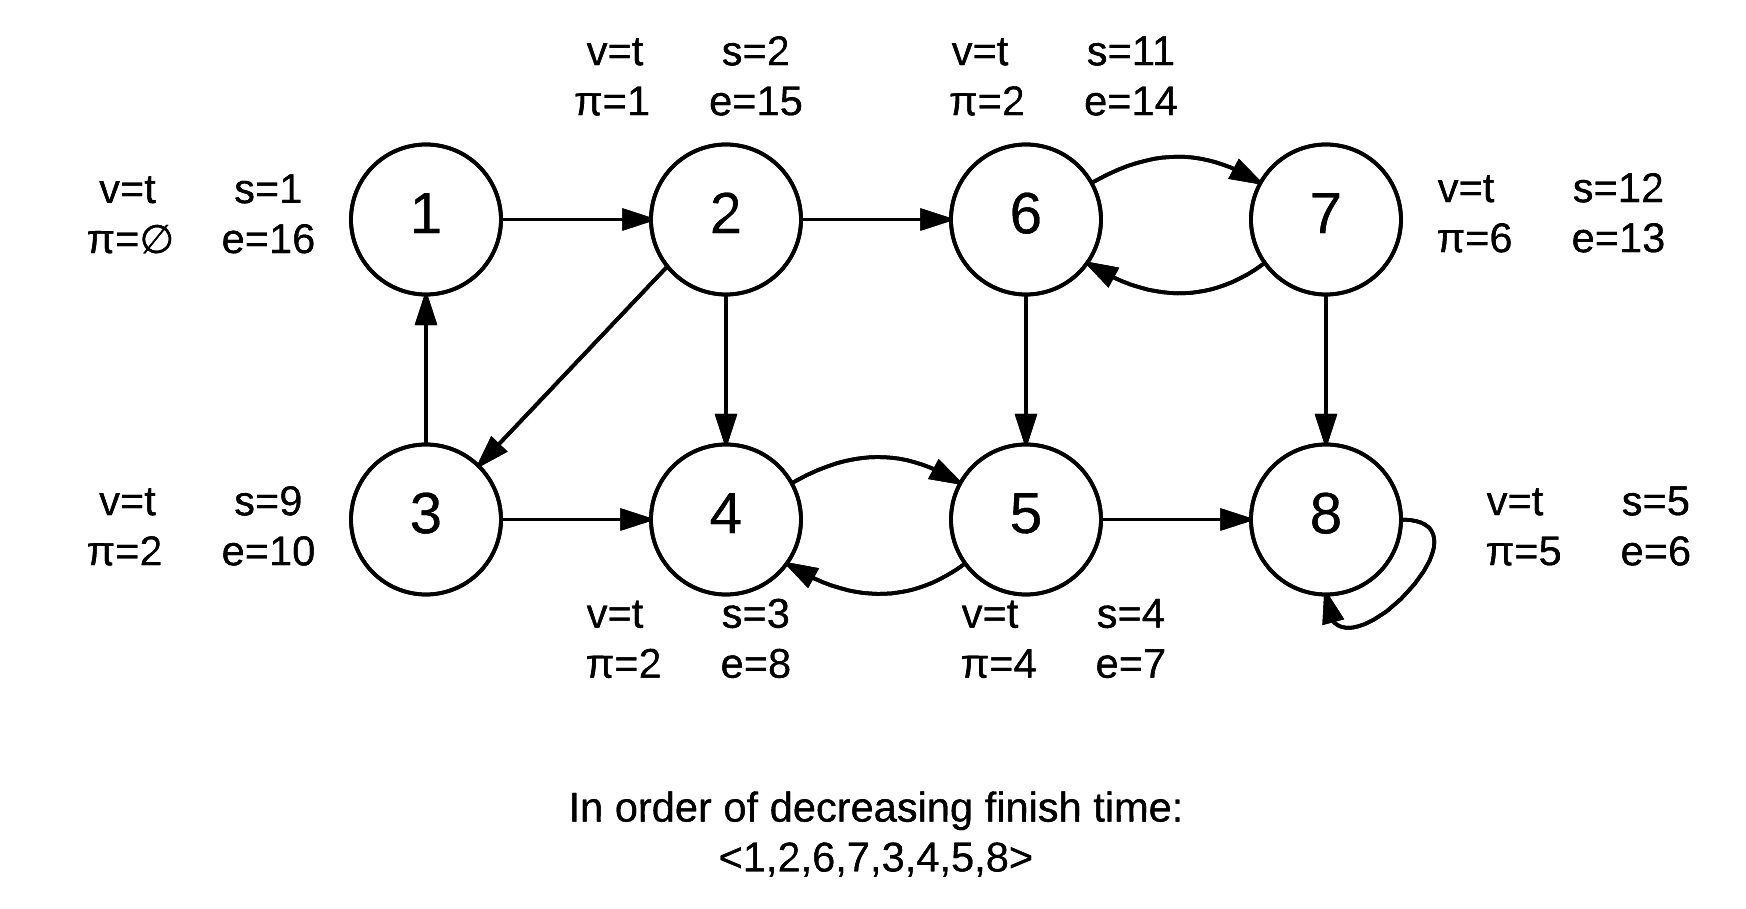
\includegraphics[width=10cm]{scccomplete1}
\caption{Execution of the modified DFS algorithm on G}
\end{figure}
\FloatBarrier
\item compute $G^T$. This is given above.
\item Execute DFS on $G^T$ such that the nodes are considered in decreasing order of finish time computed in step 1.
\item Output each tree in the DFS forest calculated in step 3 as a SCC. Each tree in the following forest represents a strongly connected component in the original graph.
\end{enumerate}
\begin{figure}[h]
\centering
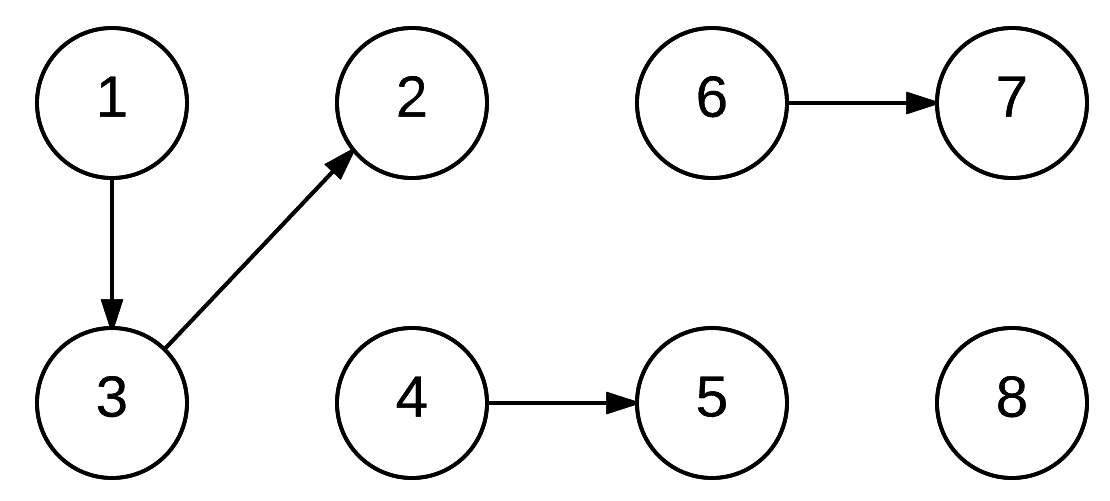
\includegraphics[width=7cm]{scccomplete2}
\caption{DFS forest resulting from the execution of the SCC finding algorithm}
\end{figure}
It can now be clearly seen that there exists 4 strongly connected components in the original graph: \{1,3,2\}, \{6,7\}, \{4,5\}, and \{8\}.
\section{Minimum Spanning Trees}
\paragraph{Problem}
There exists a set of servers which need to be connected with cables either directly or indirectly i.e. through multiple nodes, or hops. Cables have different cost, cost could be a function of length for example, and it is desired to find the minimal set of cables, and by extension cost, by which the entire set of servers may be connected. 
\begin{figure}[h]
\centering
\includegraphics[width=5cm]{mstprob}
\end{figure} 
Represent the preceding as a graph G(V,E) in which is vertex v is a server and the edges are the set of all possible cables which may connect servers. This will be a weighted graph. \\
Functions:
\begin{itemize}
\item Weight function $w : E\to \mathbb{R}^+$ each edge is assigned a weight greater than zero 
\item Find $T^*\subseteq E$: it connects all servers and has minimal possible cost.
\item Solve for $G^*=(V,T^*)$ such that the following are satisfied, given that p is a path:
\[\forall u,v\in V \exists p\subseteq T^*\] 
\[\forall e\in T^* \left( \sum_0^{|T^*|}{e} \right) \text{ is minimal}\]
Once those conditions have been satisfied, the resulting graph $G^*$ is the minimum spanning tree (MST)
\end{itemize}
\section{Kruskal's Algorithm}
\paragraph{Greedy MST} Start from an empty set of edges - S=$\emptyset$. At each iteration add the edge in the graph with minimum cost which does not create cycles in S.
\begin{algorithm}
Kruskal(G,w)\Begin{
	S=$\emptyset$\\
	\While{$\exists(u,v)\in E\setminus S:S\cup\{(u,v)\}$ does not create cycles in S}{
		let D $subseteq E\setminus S:$ each edge in D does not create cycles .if added to S\\
		$(u,v)=\underset{(p,q)\in D}{\arg\min}\hspace{2mm} {w(p,q)}$\\
		S=S$\cup$\{(u,v)\}\\
	}
	return S
}
\end{algorithm}
Before the execution of the algorithm, no nodes are connected, this is denoted by the dotted borders around them. Also, no edges are selected, this too is denoted by the dotted lines. As the algorithm iterates, edges are chosen to connect nodes, and they are darkened, until no more edges need be chosen to connect any nodes, or as long as edges may be chosen which do not create cycles. In this example, edges were chosen in the following order, after which the graph is in the final state given below:S=\{(A,C),(F,B),(A,B),(C,D),(D,H),(G,E),(G,H)\}
\begin{figure}[h]
\centering
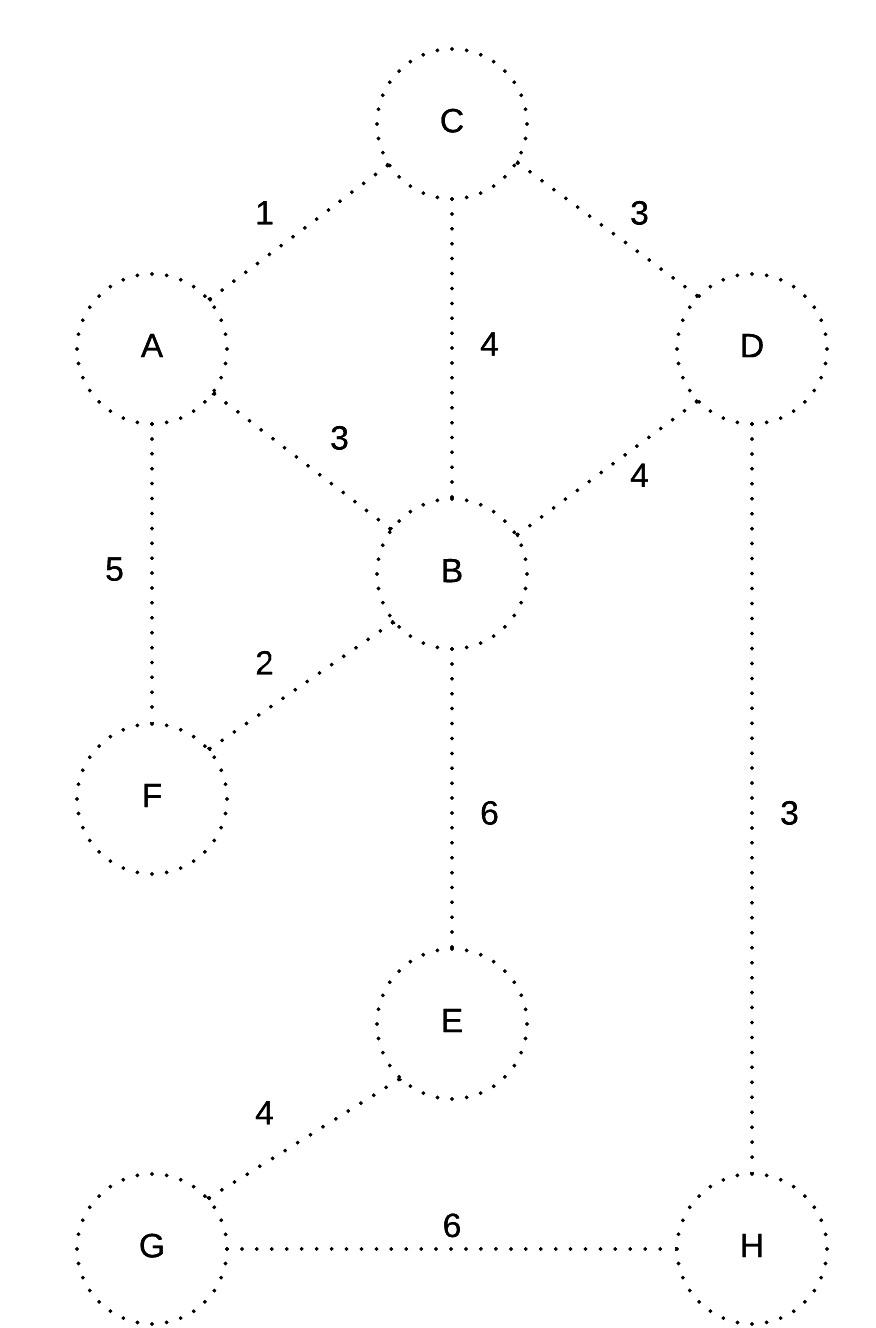
\includegraphics[width=5.56cm]{mst1}
\caption{Before Kruskal's Algorithm execution}
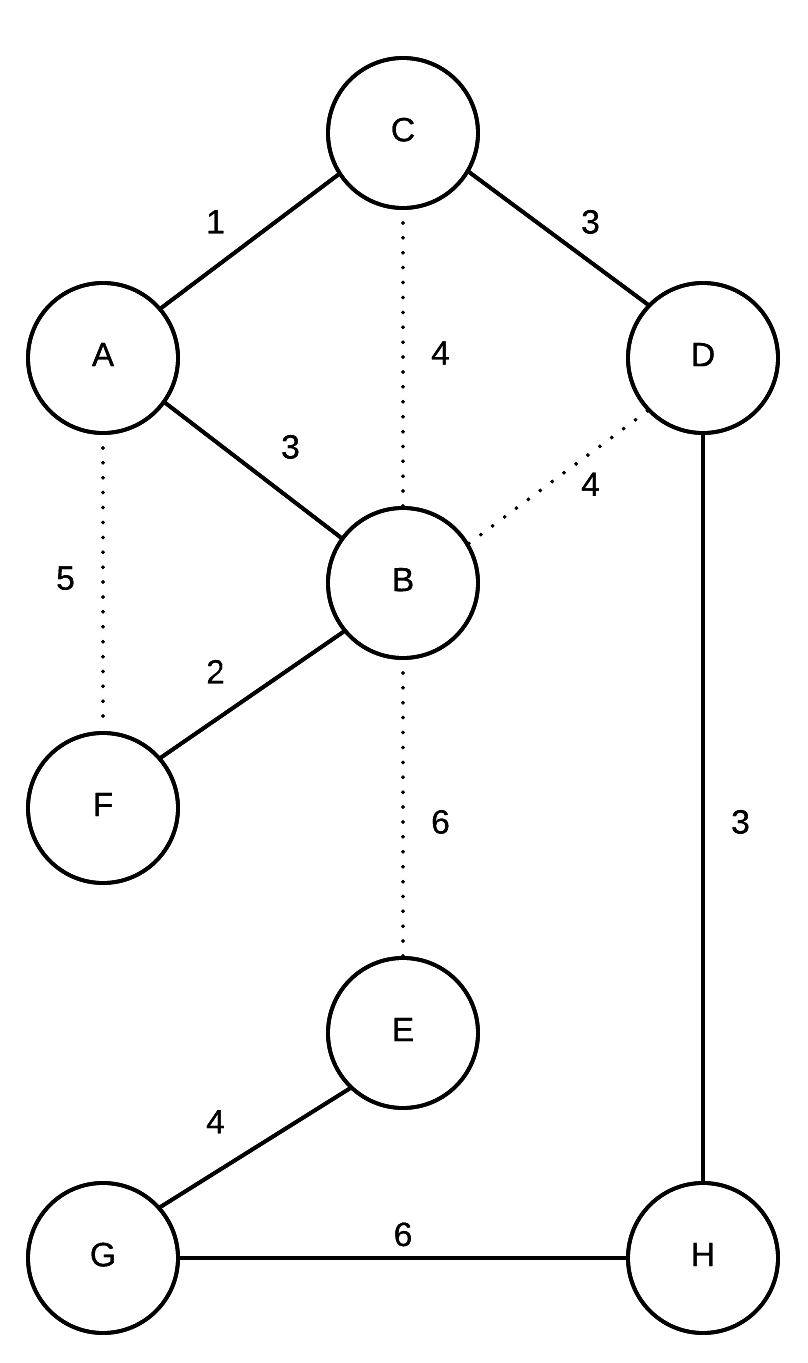
\includegraphics[width=5cm]{mst2}
\caption{After Kruskal's Algorithm execution}
\label{KruskalFin}
\end{figure}
\FloatBarrier
\subsection{Correctness of Kruskal's Algorithm}
\begin{enumerate}
\item \underline{Termination}: At each iteration, an edge is added to the solution and the loop terminates when a tree is generated. Therefore, at most, v-1 iterations will be done.
\item \underline{Induction}: Let $S_h$ be the solution at the $h^{th}$ iteration. \\ Prove that $\forall h \in \mathbb{Z}_n \exists \text{ an optimal solution }S^*:S_h\subseteq S^*$. 
\begin{itemize}
\item Base: $S_0= \emptyset \to S_0 \subseteq S^*$
\item Assume: $\exists S^*:S_h\subseteq S^*$
\item Prove: $S_{h+1}\subseteq \text{ some optimal solution }$\\Let (u,v) be the edge selected at the h+1 iteration. \\ 
If (u,v) $\in S^*$ then $S_{h+1}\subseteq S^*\to$ done. \\
Else $S^*\cup \{(u,v)\}$ would have a cycle:
\begin{figure}[h]
\centering
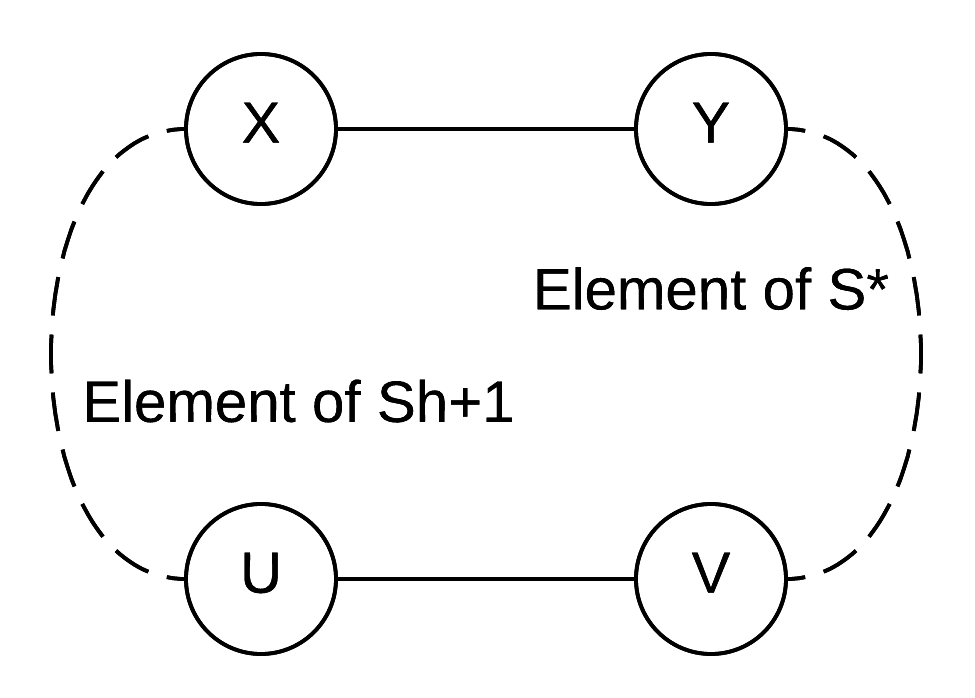
\includegraphics[width=5cm]{kruprex}
\end{figure} 
(u,v) creates a cycle when added to $S^*$ but does not create a cycle when added to $S_h$\\
Therefore there exists at least one edge (x,y) in $S^*$ which is not in $S_h$ \\
(x,y) in $S^*$ does not create a cycle since $S_h\subseteq S^* \to $ the edge (x,y) does not create a cycle in $S_h$\\
Therefor (x,y) was an edge which could have been selected by the algorithm at the h+1 iteration\\
$S^\#=(S^*\setminus \{(x,y)\})\cup \{(u,v)\}$\\
$S^\#$ has n-1 edges \\
$w(S^\#)\leq w(S^*)$\\
$\therefore S^\#$ is optimal and $S_{h+1}\subseteq S^\#$
\item Final Solution is optimal\\
The solution has n-1 edges\\
There exists an optimal solution $S^*:S_{n-1}\subseteq S^*$\\
$|S^*=n-1$\\
$|S{n-1}|=n-1$\\
Therefore $S_{n-1}$ is optimal
\end{itemize}
\end{enumerate}
\subsection{Efficient Implementation of Kruskal's Algorithm}
\begin{itemize}
\item Sort edges in ascending order by weight
\item The set of selected edges till the current iteration identifies a set of connected components
\item An edge creates a cycle if it connects two nodes in the same component
\item An array E is used for each edge i:
\begin{itemize}
\item E[i].u and E[i].v are the endpoints
\item E[i].w is the weight of the edge
\end{itemize} 
\item An array CC[i$\dots$n] where n is the number of nodes in the graph - $|V|$. CC[i] is the id of the connected component of node i. Initially, $CC[i]=i\forall i\in [1\dots n]$
\end{itemize}
\subsection{Efficient Kruskal Implementation Pseudocode}
\begin{algorithm}[h]
Kruskal(G,w)\Begin{
	S=$\emptyset$\\
	m=$|E|$\\
	Sort E ascending by weight \\
	\For{i=1 to n}{
		CC[i]=i
	}
	\For{j=1 to m}{
		(u.v)=(E[j].u,E[j].v)\\
		\If{CC[u]$\neq$CC[v]}{
			S=S$\cup$\{(u,v)\}\\
			cid=CC[v]\\
			\For{p$\in$V}{
				\If{CC[p]==cid}{
					CC[p]=CC[u]
				}
			}
		}
	}
	return S
}
\end{algorithm}
The complexity of this algorithm is:
\[\Theta(m\log m+m+n^2=\Theta(m\log m +n^2\]
The additive m is dropped in the simplification since m can be as much as $n^2$ and $\theta$ is concerned only with asymptotic behavior.
\FloatBarrier
\section{Prim's Algorithm}
Prim's is a greedy algorithm which also solves the minimum spanning tree, through from a slightly different logical approach to the problem. It has a root node, and at each iteration it extends the tree rooted at the root node by selecting the edge with minimum weight that connects a node in the tree with a node that is not yet in the tree. The algorithm terminates when all nodes belong to the tree, and that tree will be the minum spanning tree. 
\subsection{Prim's Algorithm Pseudocode}
\begin{algorithm}[h]
Prim(G,w)\Begin{
	S=$\emptyset$\\
	select a node r $\in$ V as the root\\
	C=\{r\}//nodes currently in the tree\\
	\While{C$\neq$V}{
		$(u,v)=\underset{\substack{(x,y)\in E:\\x\in C \wedge y\ni C }}{\arg\min}\hspace{2mm} {w(x,y)}$\\
		S=S$\cup$\{(u,v)\}\\
		C=C$\cup$\{v\}
	}
	return S
}
\end{algorithm}
\FloatBarrier
It can be demonstrated that for any graph with only positive weights, both Prim's and Kruskal's algorithms will yield the same tree. Students may find it instructive to work the same graph problem with both algorithms to solidify this fact, and the differences in their logical execution. 
\subsection{Efficient Implementation of Prim's Algorithm}
\begin{algorithm}[h]
Prim(G,W,r)\Begin{
	\For{$v\in V$}{
		v.$\pi$=NULL\\
		v.d=$\infty$
	}
	r.d=0\\
	Q=V //set of unvisited nodes\\
	\While{Q$\neq \emptyset$}{
		v=Q.ExtractMin()\\
		\For{u$\in$ adj(v)}{
			\If{$u\in Q \wedge u.d>(v,u)$}{
				u.$\pi$=v\\
				u.d=w(v,u)
			}
		}
	}
}
\caption{Pseudo Code for an efficient implementation of Prim's Algorithm}
\end{algorithm}
\FloatBarrier
Iterating through the algorithm, given the same graph used earlier in discussion of Kruskal (Figure \ref{KruskalFin}), yields the following table of choices enumerated over the loop iterations, given that node A is specified as the root.
\begin{figure}[h]
\centering
\begin{tabular}{|c|c|c|c|c|c|c|c|c|c|}
\hline
 &Q=&A&B&C&D&E&F&G&H\\ \hline \hline
 &init&0&$\infty$&$\infty$&$\infty$&$\infty$&$\infty$&$\infty$&$\infty$\\ \hline
1&Select A&\st{0}&3&1&$\infty$&$\infty$&5&$\infty$&$\infty$\\ \hline
2&Select C&\st{0}&3&\st{1}&3&$\infty$&5&$\infty$&$\infty$\\ \hline
3&Select B&\st{0}&\st{3}&\st{1}&3&6&2&$\infty$&$\infty$\\ \hline
4&Select F&\st{0}&\st{3}&\st{1}&3&6&\st{2}&$\infty$&$\infty$\\ \hline
5&Select D&\st{0}&\st{3}&\st{1}&\st{3}&6&\st{2}&$\infty$&3\\ \hline
6&Select H&\st{0}&\st{3}&\st{1}&\st{3}&6&\st{2}&6&\st{3}\\ \hline
7&Select G&\st{0}&\st{3}&\st{1}&\st{3}&4&\st{2}&\st{6}&\st{3}\\ \hline
8&Select E&\st{0}&\st{3}&\st{1}&\st{3}&\st{4}&\st{2}&\st{6}&\st{3}\\ \hline
\end{tabular}
\caption{Iterative Execution of Prim's Algorithm given in a table}
\end{figure}
\FloatBarrier
Take note that in step 7 the algorithm had a choice, two edges were available of equal weight. In this case, one was chosen arbitrarily, but if you were to follow the other path in the execution of the algorithm, it too would have yielded a different, but still optimal solution. The resulting graph of the minimum spanning tree, which is the same as the one yielded for this graph when Kruskal's algorithm was applied, is given below. 
\begin{figure}[h]
\centering
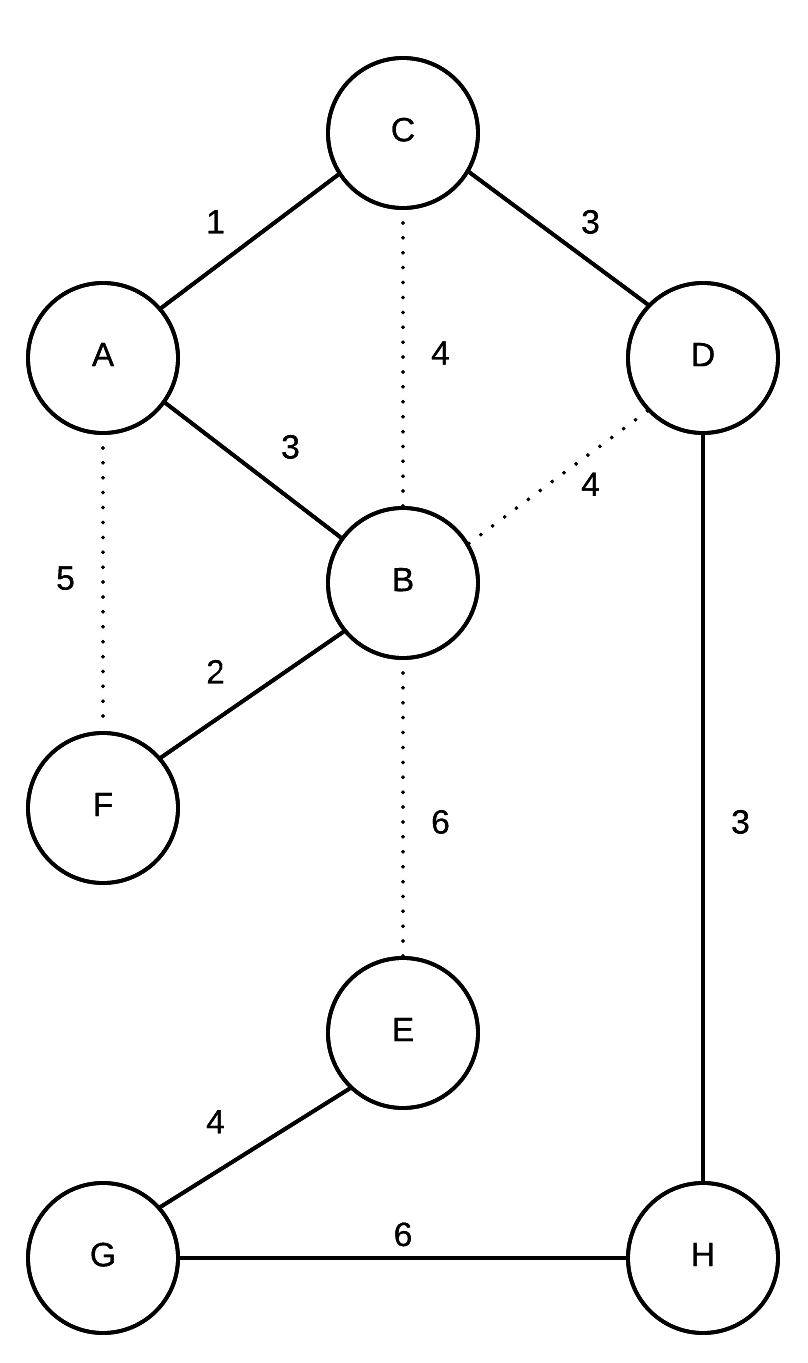
\includegraphics[width=5cm]{mst2}
\caption{Graph of the Minimum Spanning Tree generated from Prim's Algorithm}
\end{figure}
\FloatBarrier
\section{Single Source Shortest Paths}
There exists a network of servers connected by links, and each link has an associated delay. A router has to figure out the best path to the destination: the path with least delay. This can be modeled with a weighted graph G=(V,E) such that V represents the set of routers and E the set of links between routers with the weight function $w : E\to \mathbb{R}^+$, w(u,v) is the delay in the link $(u,v)\in E$.
\paragraph{Problem:} Given a source $s\in V$ find the shortest path to all other nodes in the network. 
\begin{definition}[Path Weight]\hfill \break
Given a path $p=(v_1, v_2,\dots v_k)$ the weight of p is the sum: 
\[\sum_{i=1}^{k-1}{w(v_i,v_{i+1})}\]
\end{definition}
\begin{definition}[Shortest Path]\hfill \break
The shortest path between two nodes u and v is defined as $\delta (u,v)$ 
\[\delta (u,v)=\begin{cases}\underset{p:u \to v}{\arg\min} \hspace{1mm} w(p) & \text{if u and v are connected}\\ \infty & otherwise\end{cases}\]
\end{definition}
\subsection{Optimality Principle}
Given two nodes u and v, their shortest path p, and a node q in their shortest path, then $p'$, the path between u and q is also the shortest path for these two nodes. 
\subsection{Proof of the optimality principle by contradiction}
\begin{itemize}
\item Assume $p'$ is \textbf{not} the shortest path which exists between nodes u and q, and that $p'''$ denotes the path from q to v.
\item This implies that there exists another path $p''$ which is shorter. 
\item It follows that $w(p'')<w(p')$ and $w(p)=(w(p')+w(p'''))>w(p'')+w(p''')$
\item This leads to a contradiction because p is not the shortest available path from u to v.
\end{itemize}
Combining all shortest paths from a source to all destinations is the shortest path tree, which is the goal of the following algorithms
\section{Dijkstra's Algorithm for a shortest paths tree}
\begin{itemize}
\item Greedy approach for calculating the shortest paths tree given a source node, for that node. 
\item Starts from the source node and extends the tree by adding nodes and corresponding edges.
\item Let R be the set of nodes currently in the tree (up to the current iteration). The algorithm selects the edge (u,v) as follows:
\[(u,v):e\in R \wedge v \ni R \wedge [\delta (u) +w(u,v)] \text{ is minimal} \] 
\item Attributes for a node u
\begin{itemize}
\item u.d - is the distance from the source in the shortest paths tree. For the source, s, $s.d=0$.
\item $u.d=\delta(s,u)$
\item $u.\pi$ is the parent of u in the shortest paths tree
\item R is the set of nodes in the tree.
\end{itemize}
\end{itemize}
\begin{algorithm}[h]
DIJKSTRA(G,w,s)\Begin{
	s.d=0\\
	s.$\pi$=NULL
	R=$\{ s \}$\\
	\While{$\exists (u,v)\in E : u\in R \wedge v \ni R$}{
		$(u,v)=\underset{\substack{(x,y)\in E: \\ x \in R \\  y \ni R}}{\arg\min} \hspace{1mm} (x.d+w(x,y))$\\
		v.d=u.d+w(u,v)\\
		v.$\pi$=u\\
		R=R$\cup $\{v\}
	}
}
\end{algorithm}

\begin{figure}
\centering
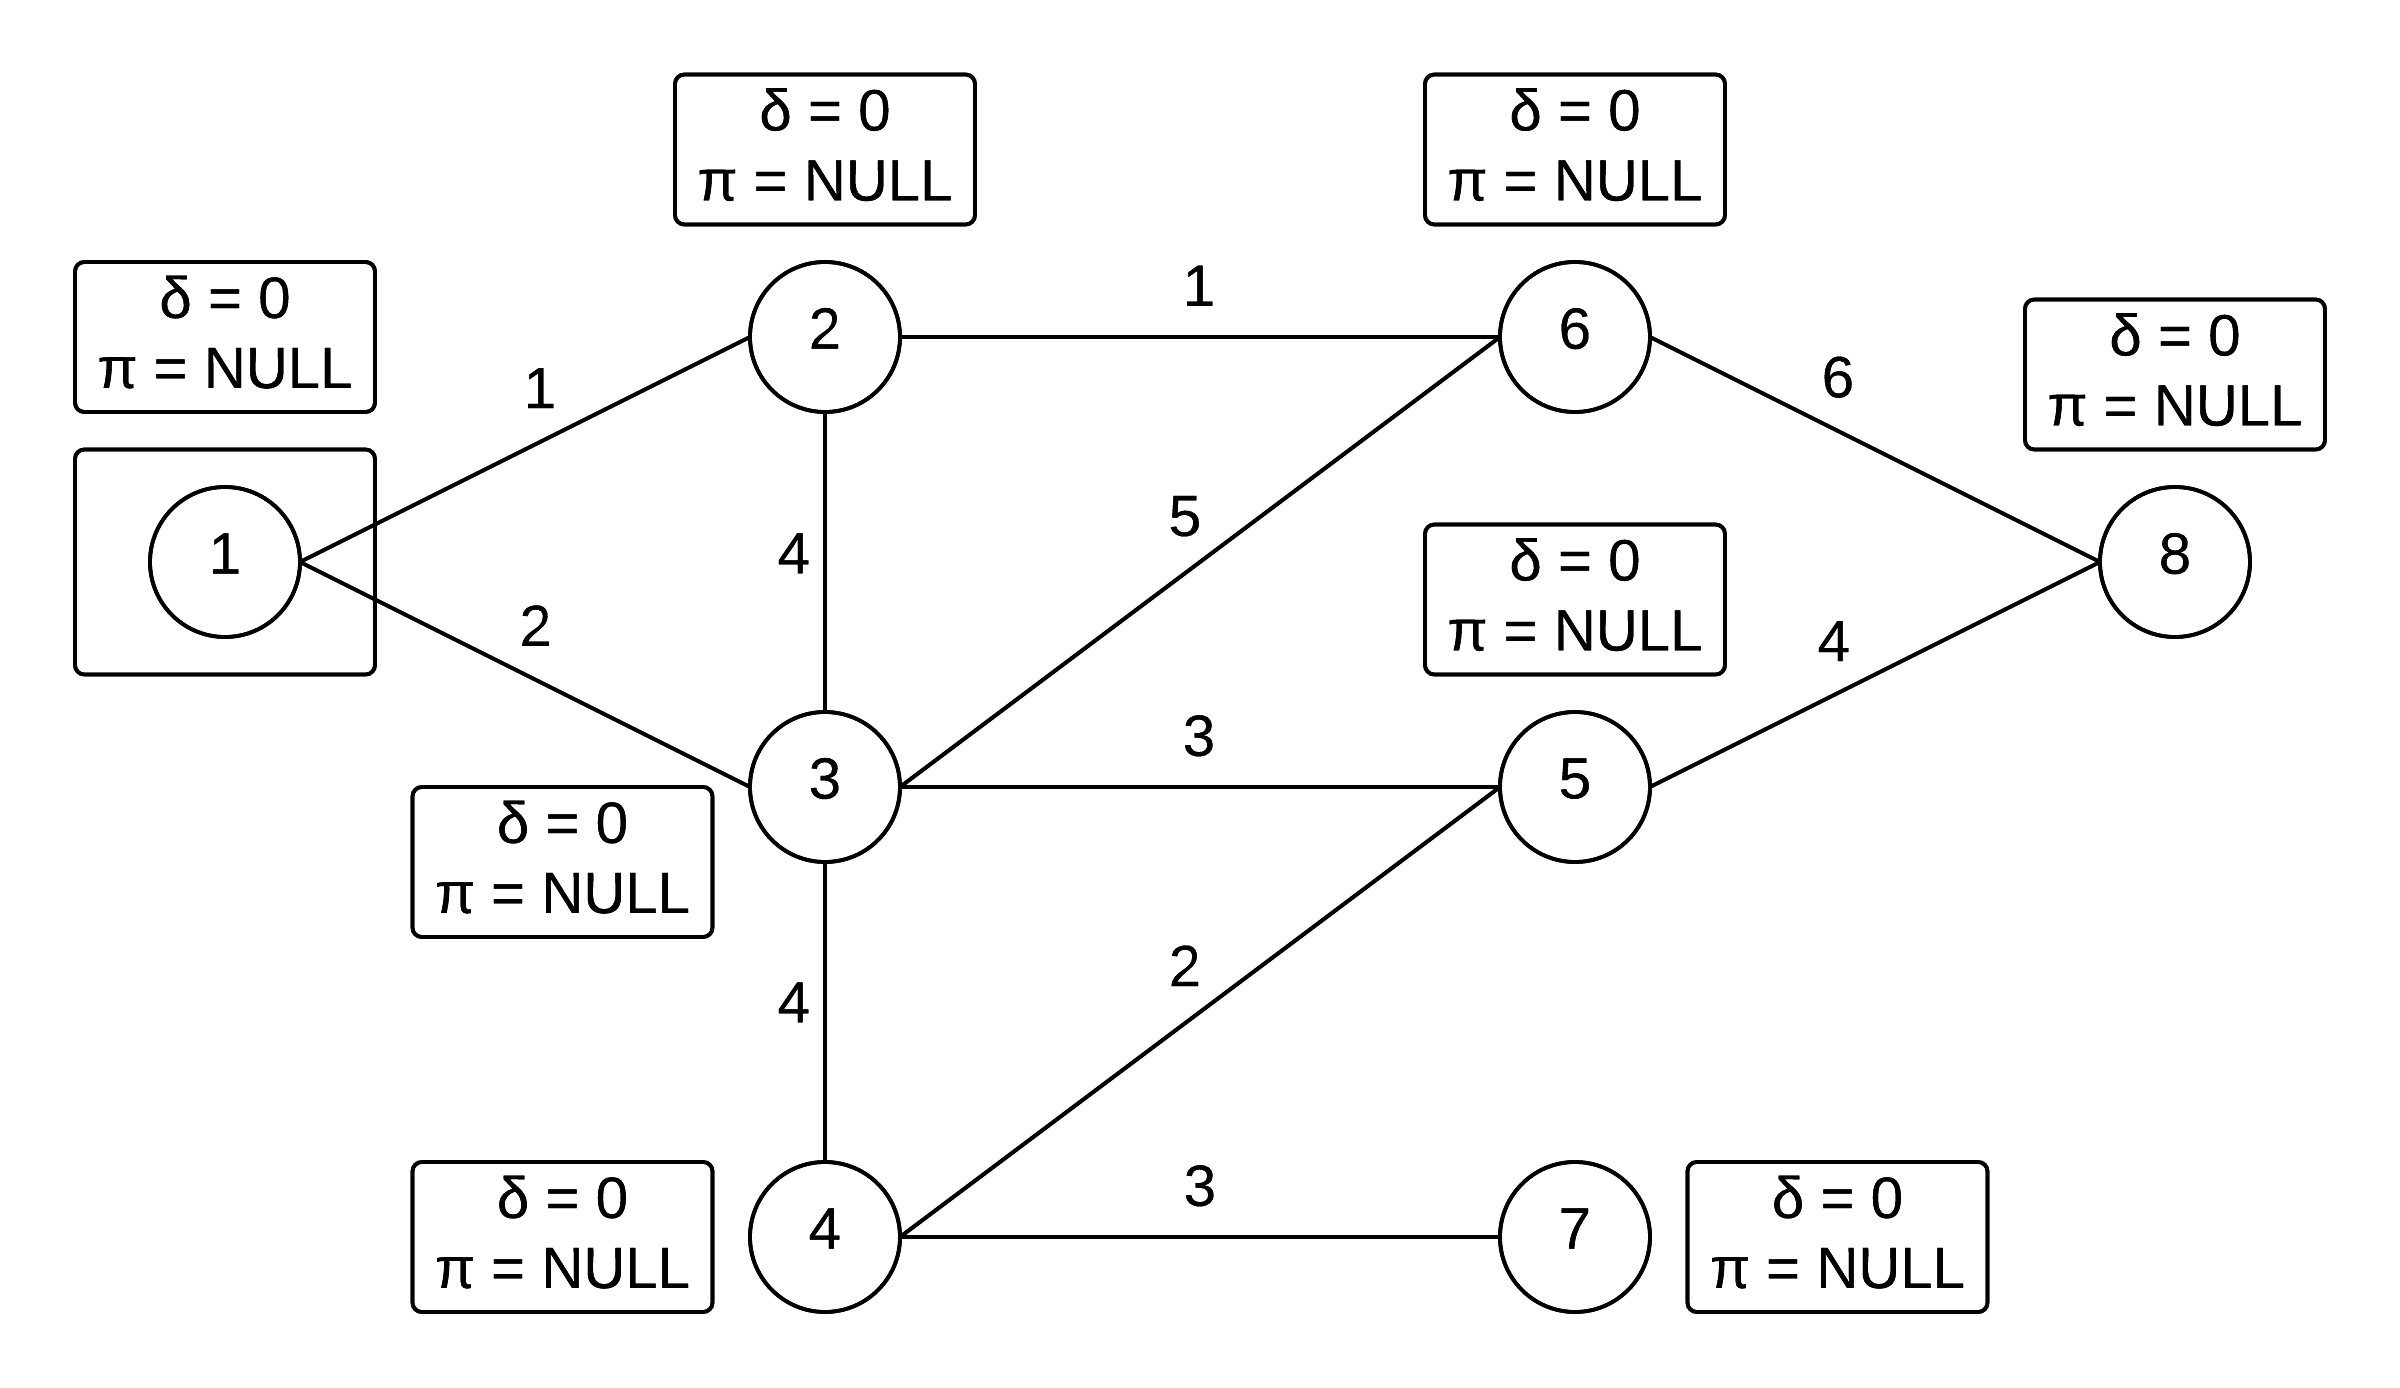
\includegraphics[width=12cm]{d0}
\caption{Initial state of graph}
\end{figure}

\begin{figure}
\centering
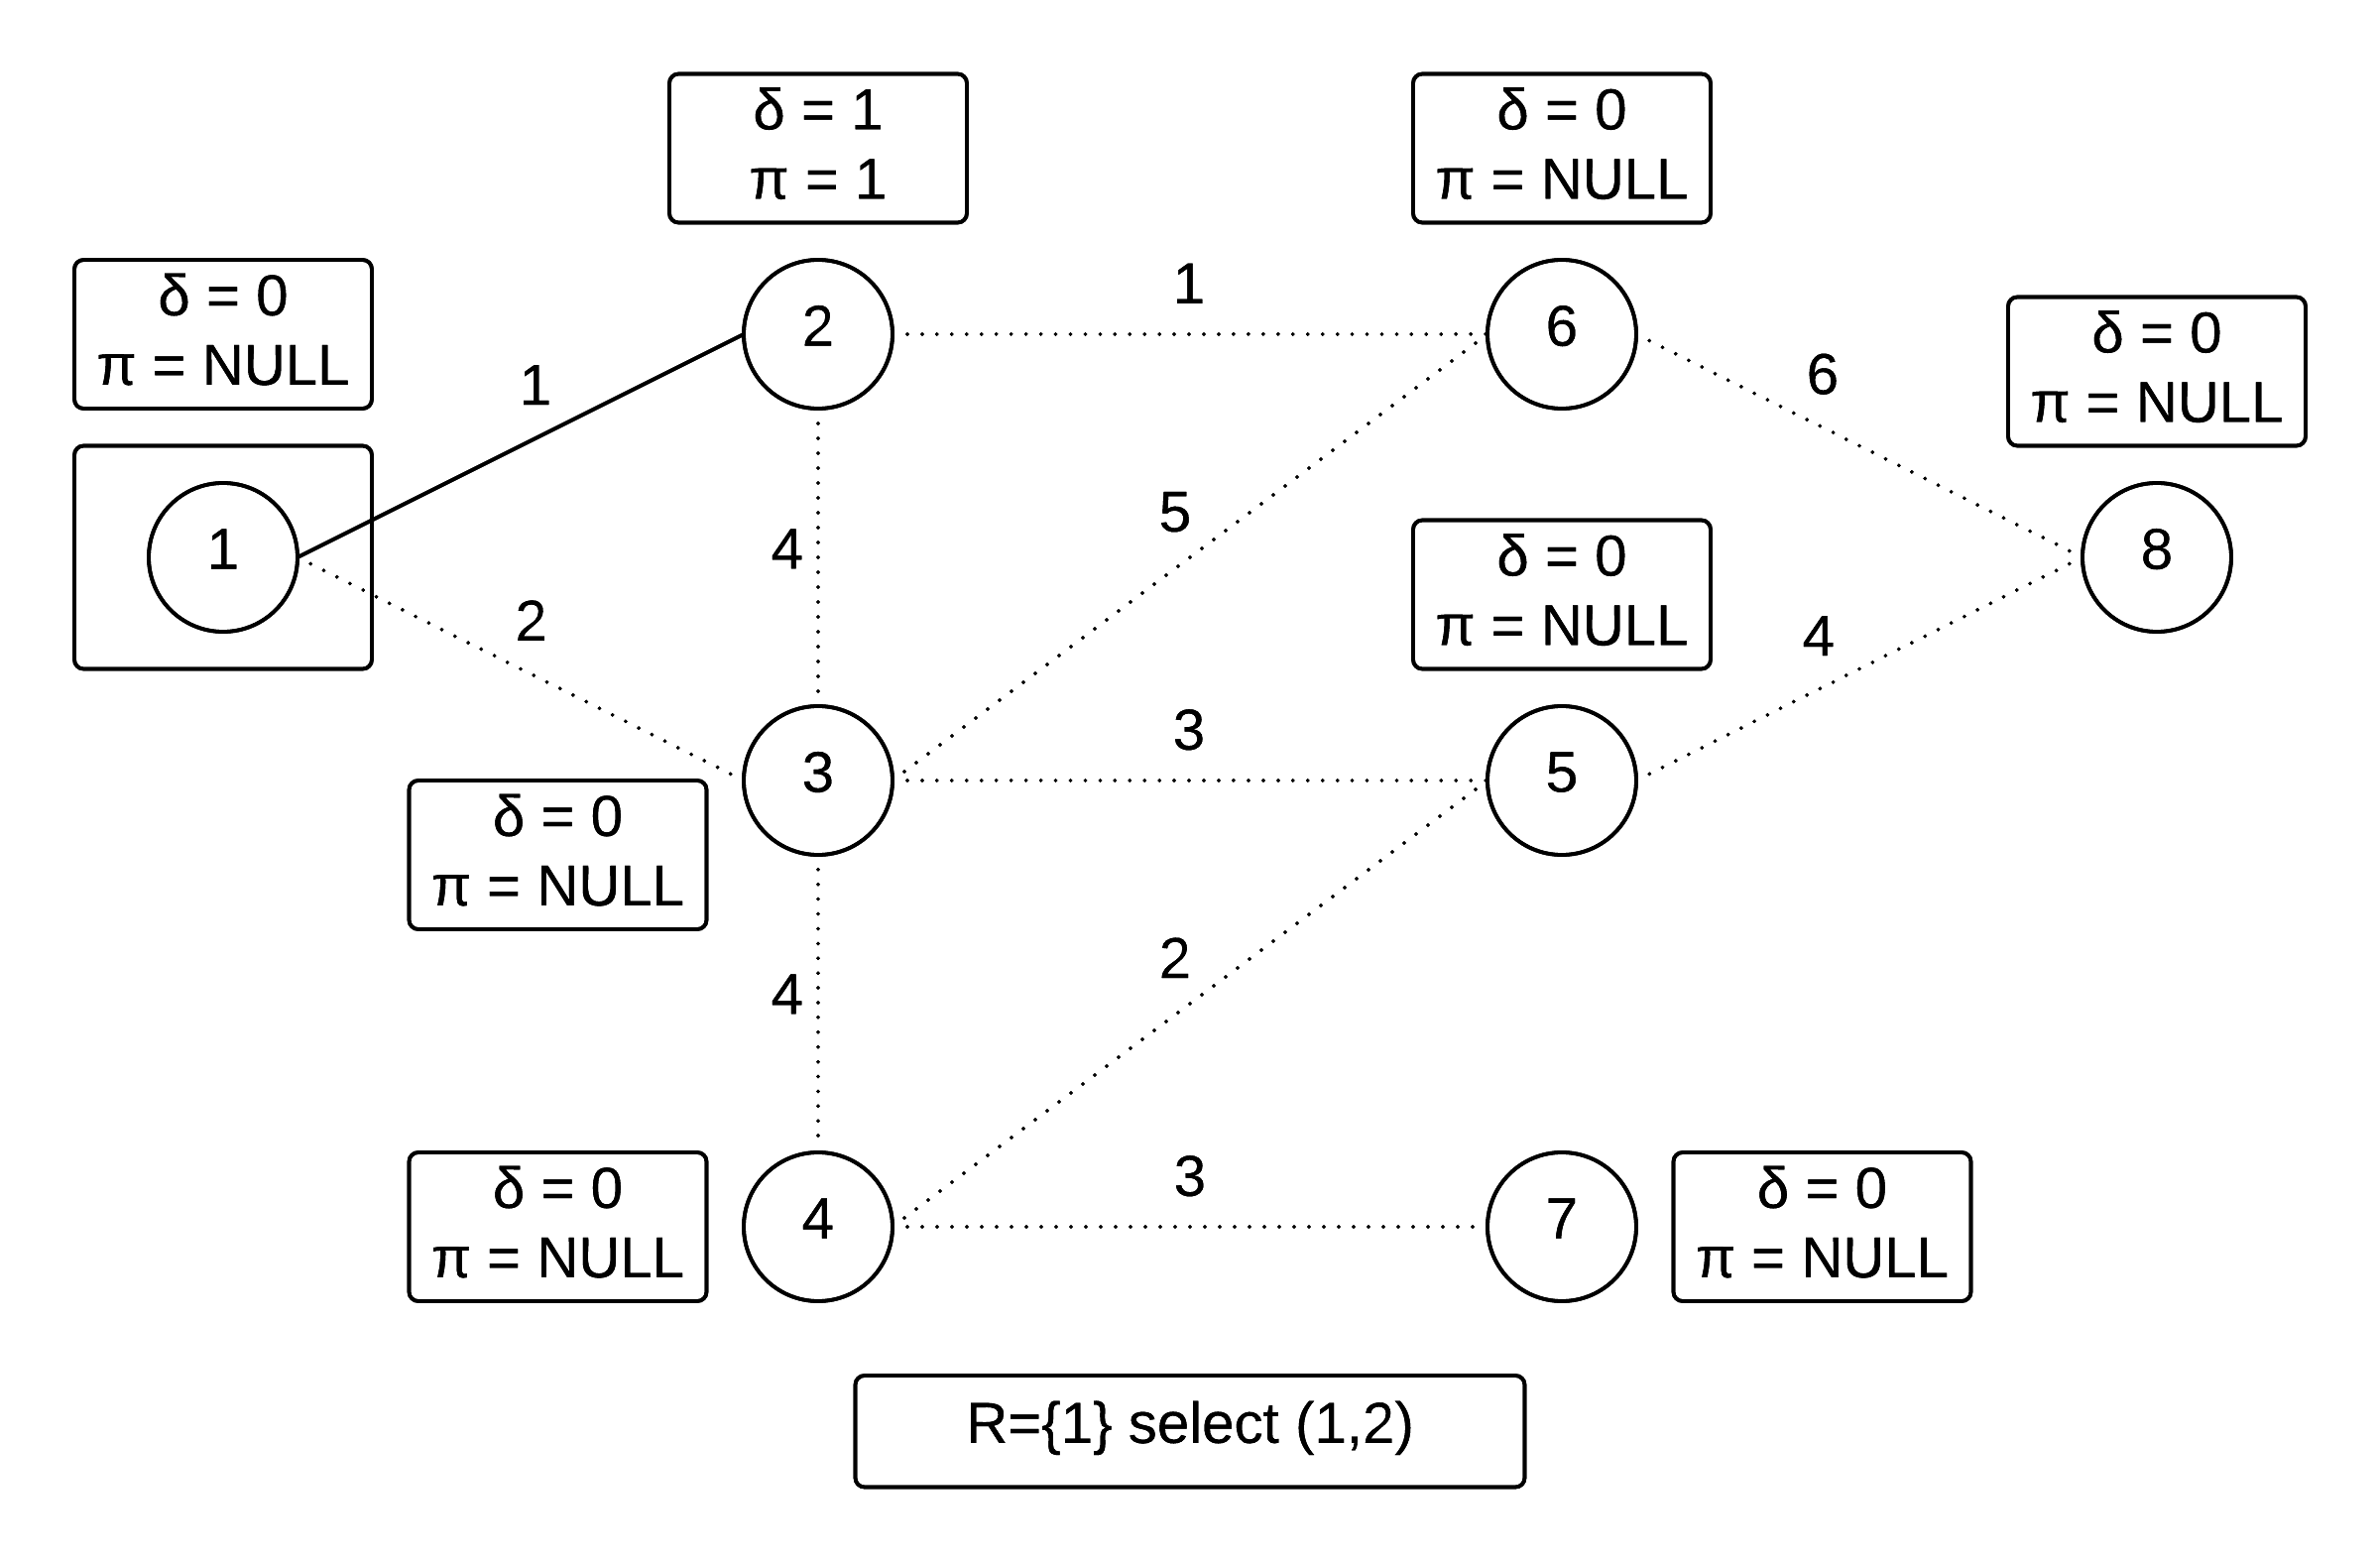
\includegraphics[width=12cm]{d1}
\caption{Step one of execution}
\end{figure}

\begin{figure}
\centering
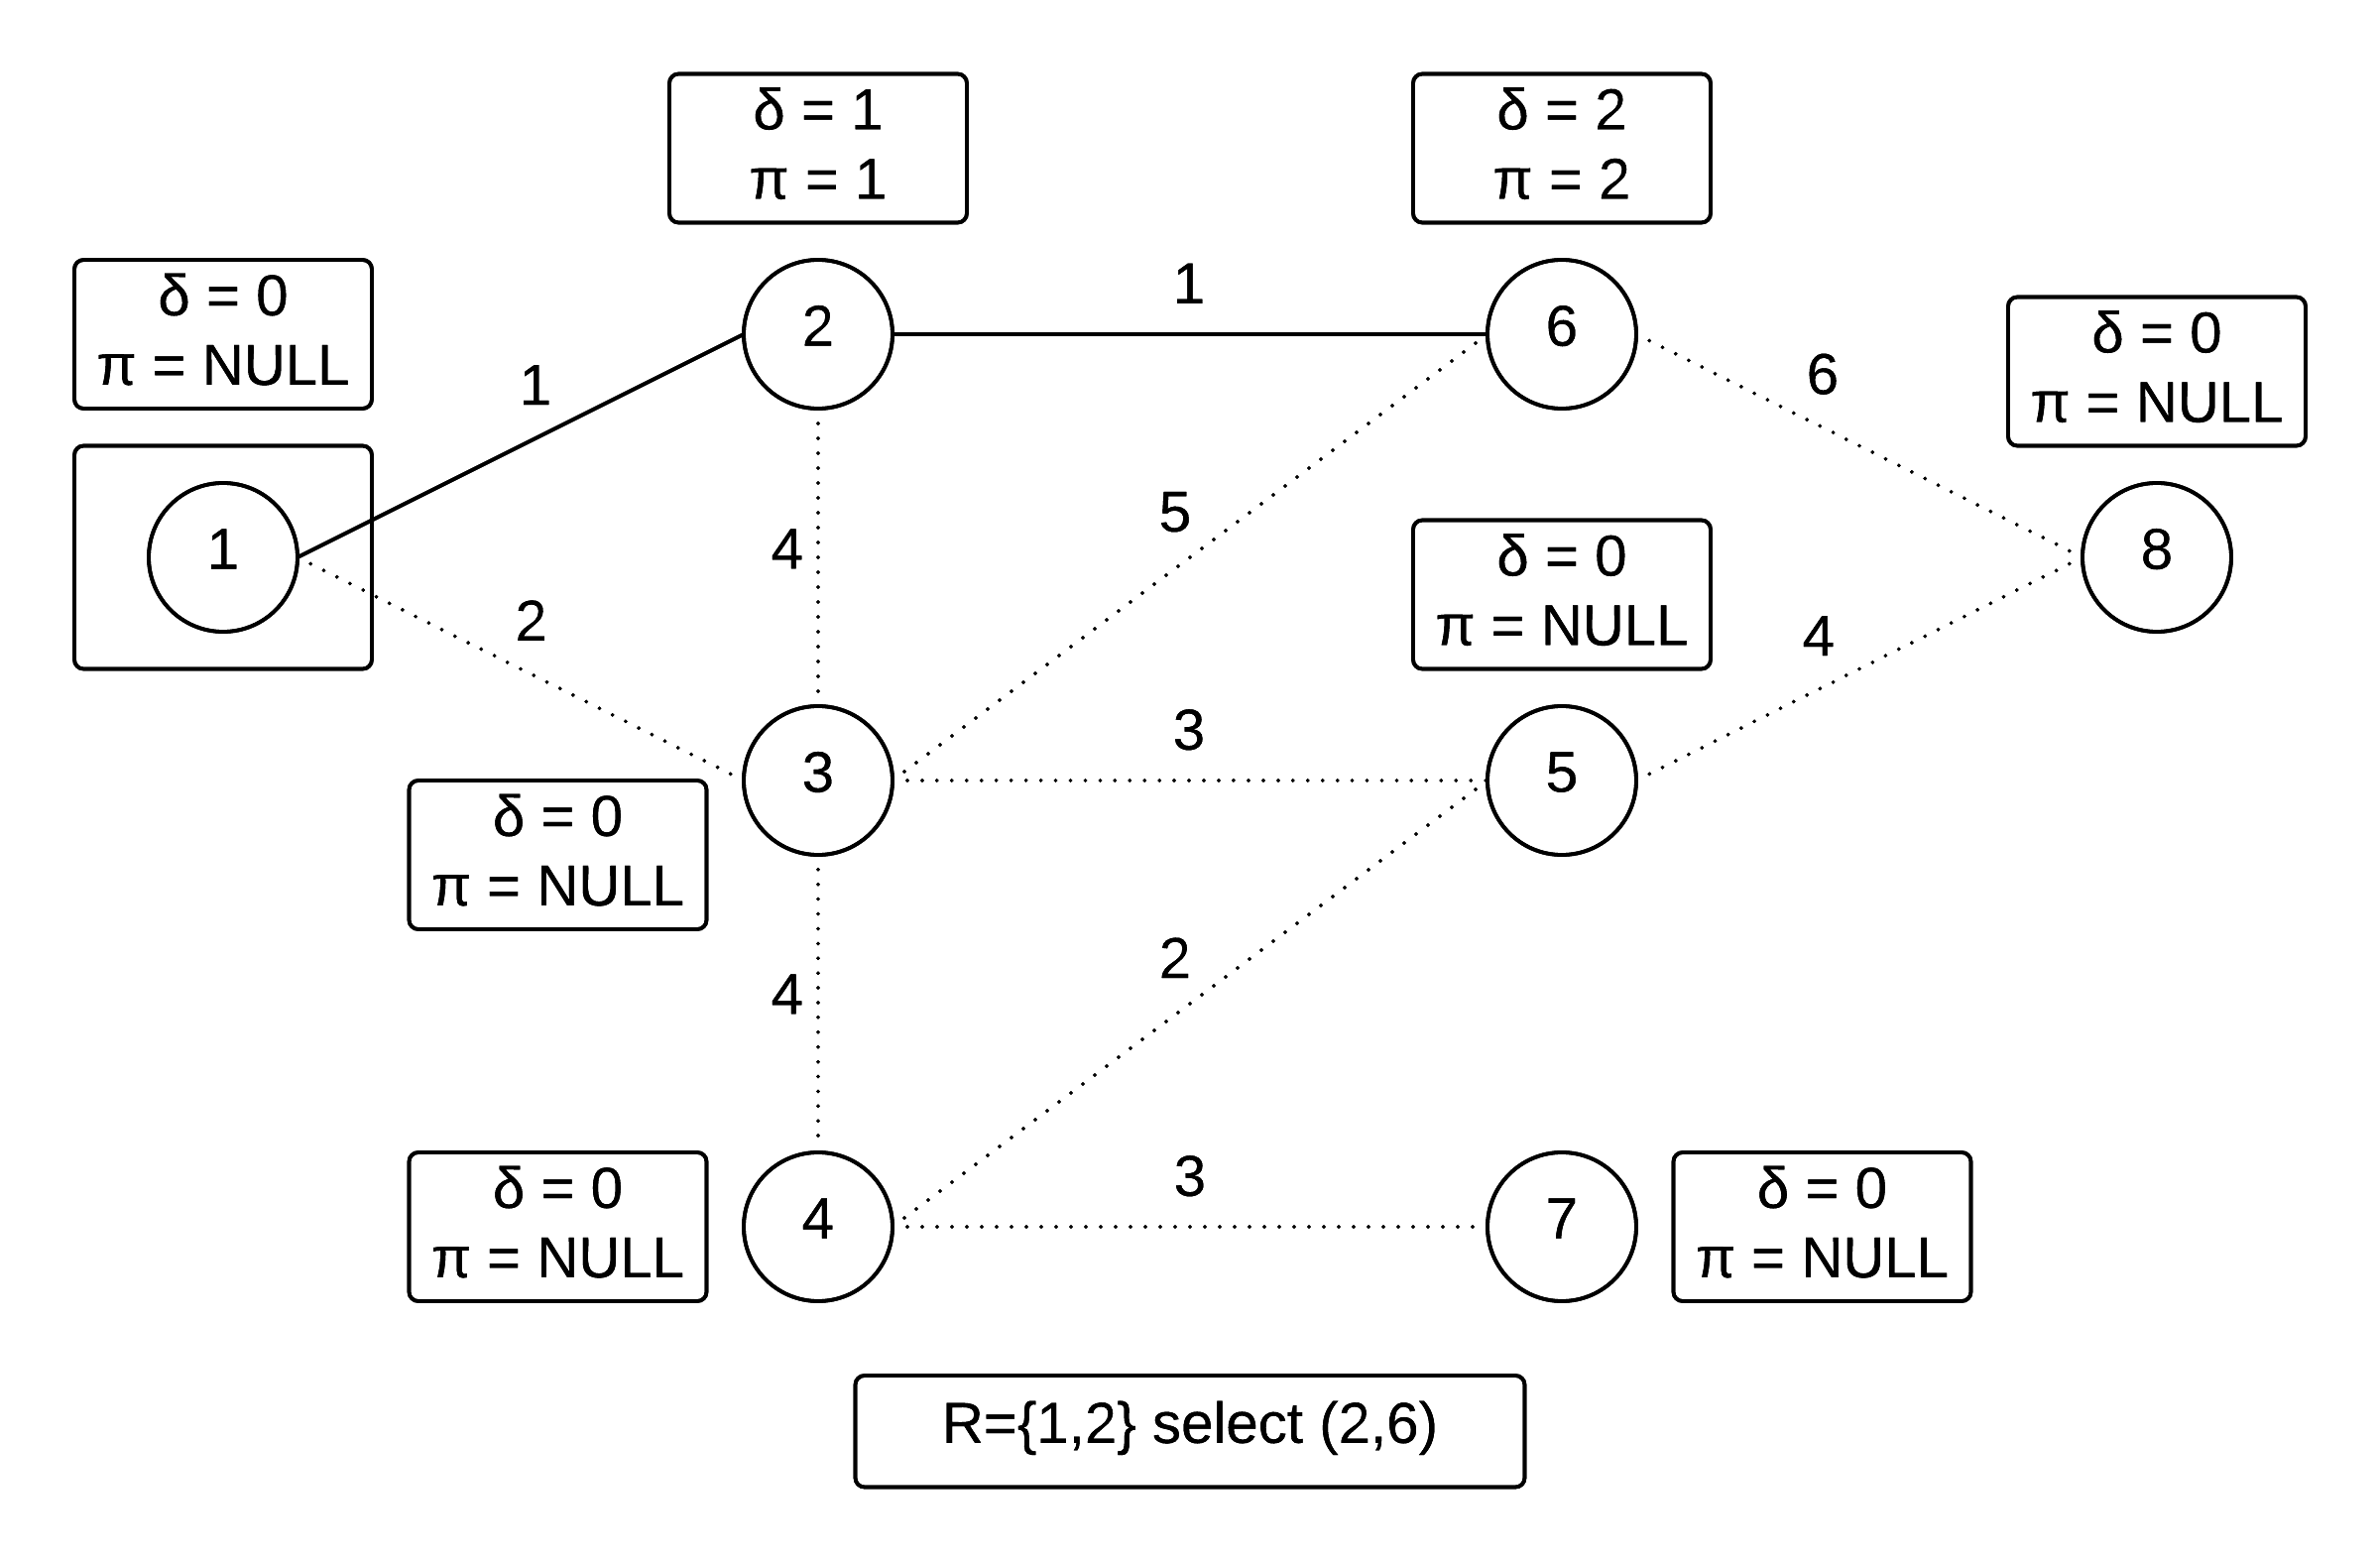
\includegraphics[width=12cm]{d2}
\caption{Step two of execution}
\end{figure}

\begin{figure}
\centering
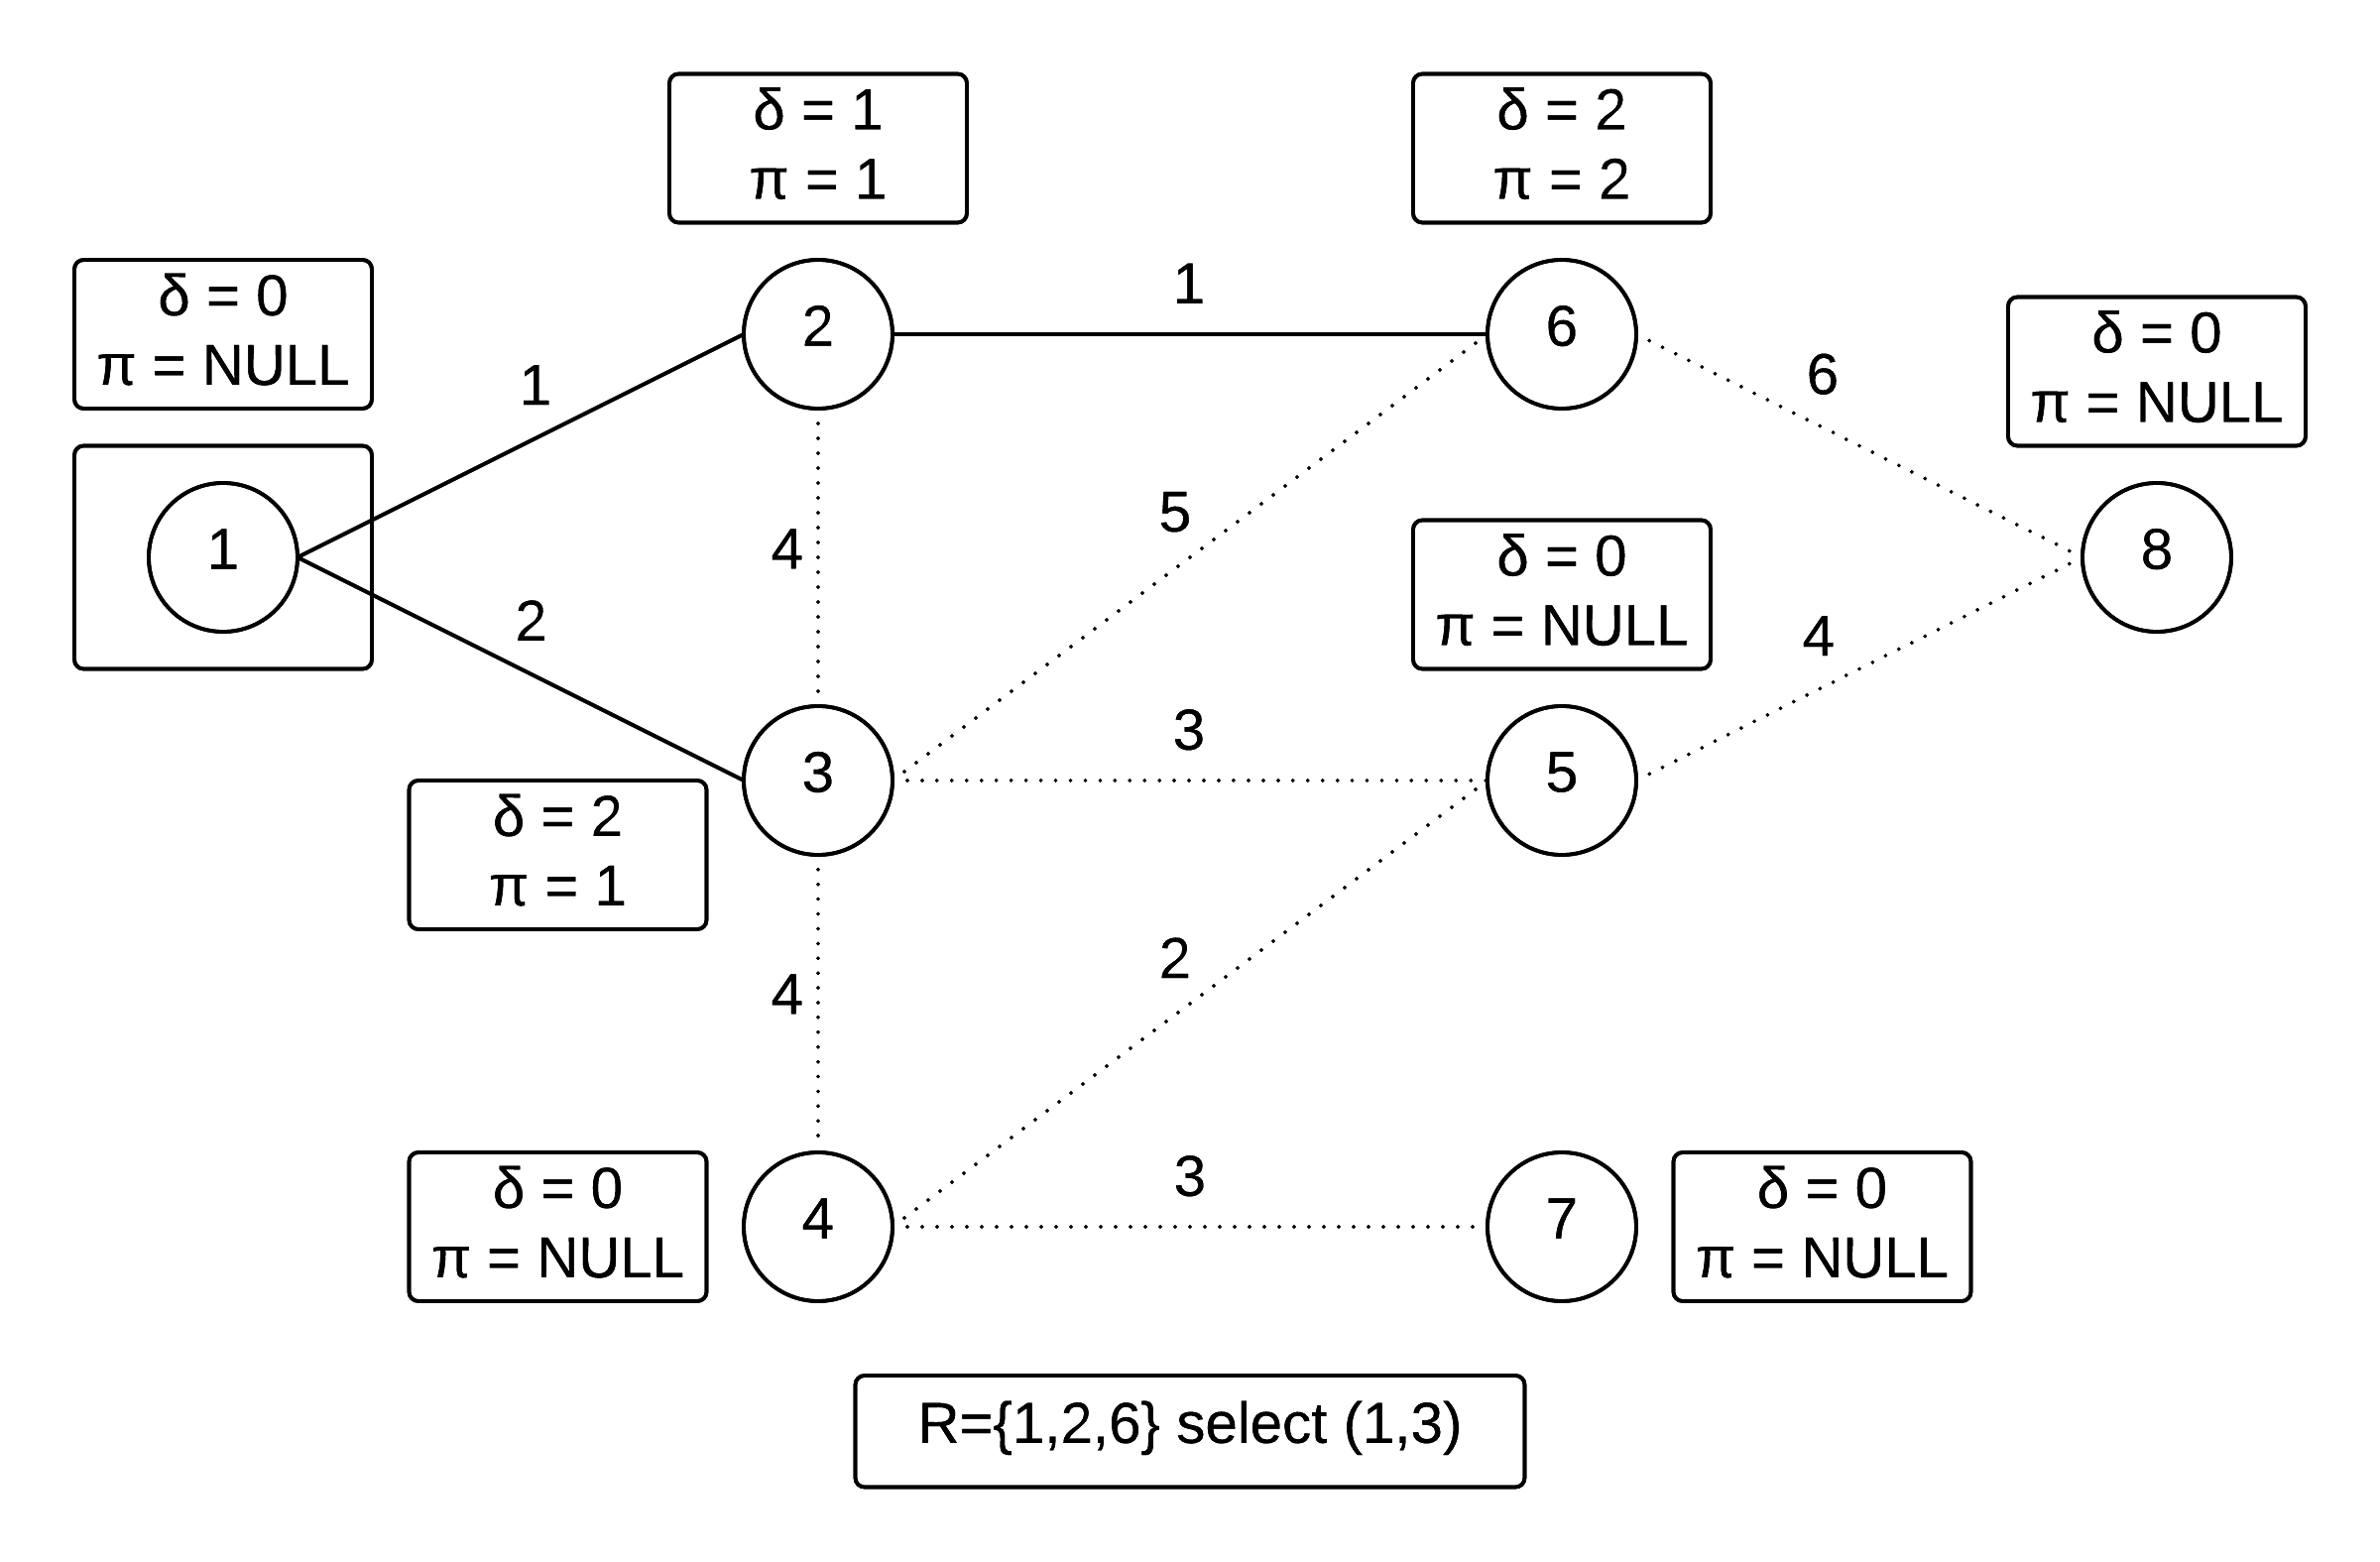
\includegraphics[width=12cm]{d3}
\caption{Step three of execution}
\end{figure}

\begin{figure}
\centering
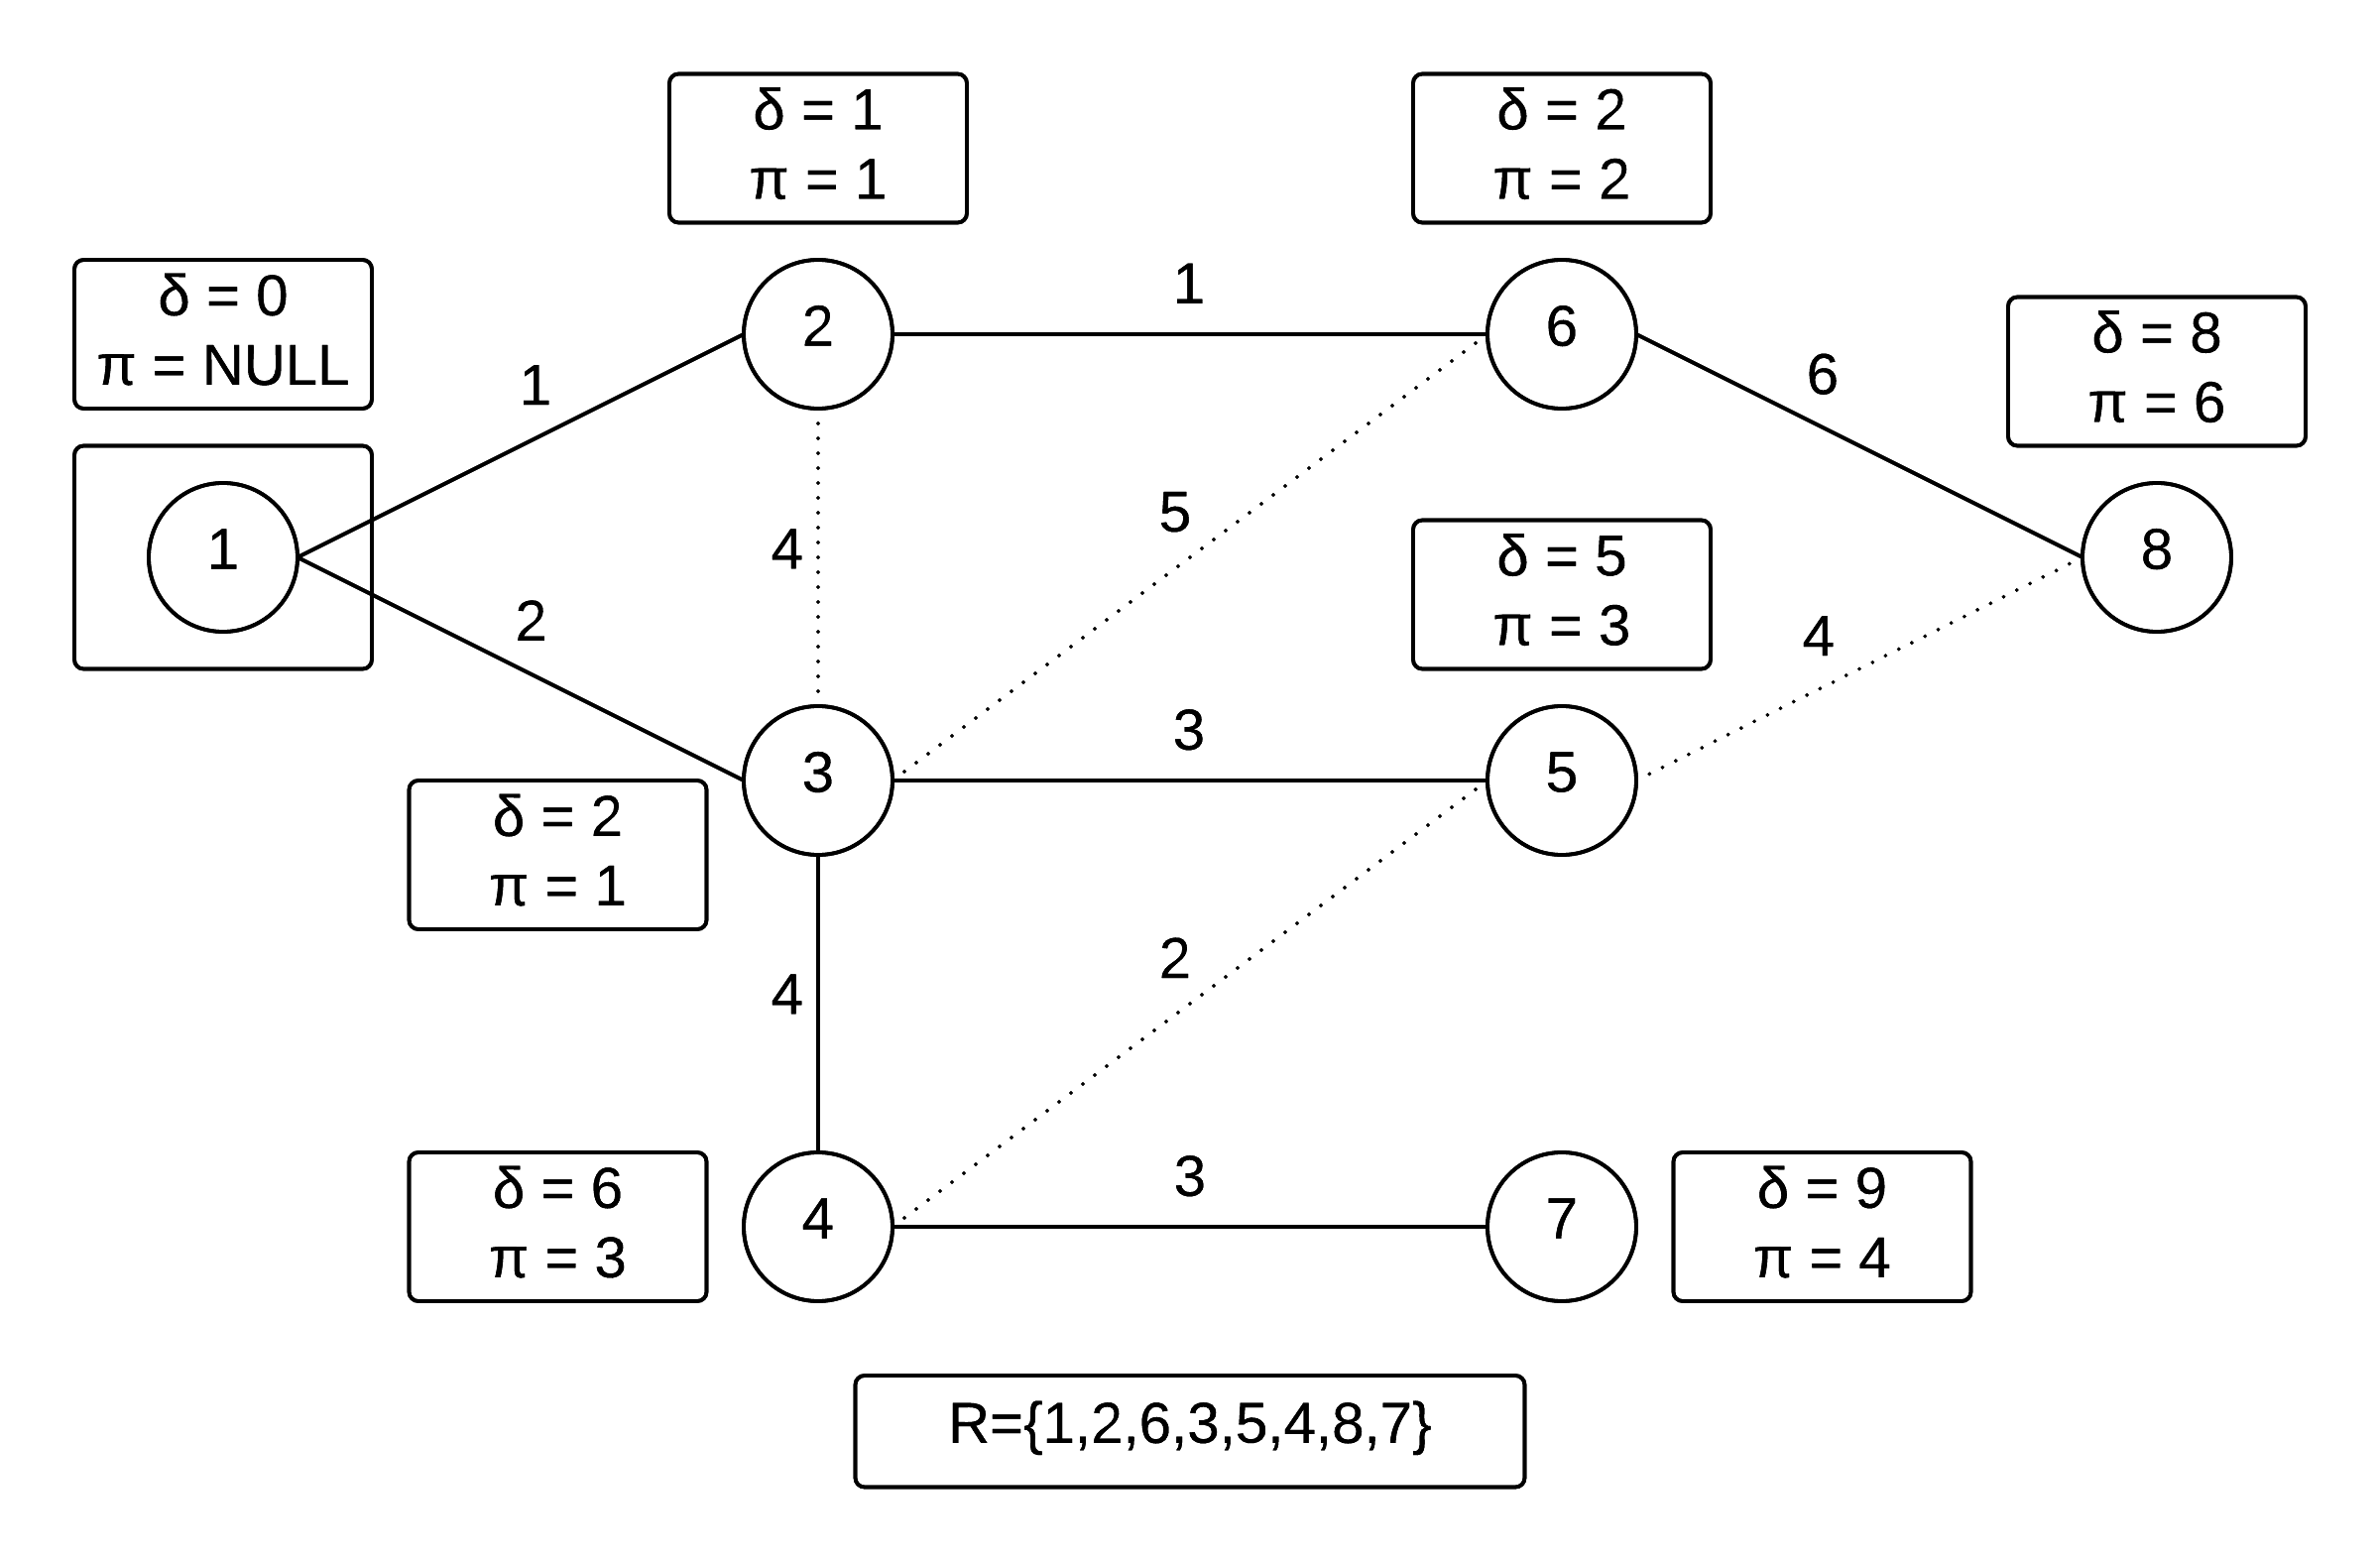
\includegraphics[width=12cm]{dfin}
\caption{Final state}
\end{figure}
\FloatBarrier
\subsection{Efficient Implementation of Dijkstra's Algorithm}
\begin{itemize}
\item Use a boolean array, to indicate $i\in R$
\[visited[1...n]:v[i]=\begin{cases}true & \text{if it the vertex has been visited by the algorithm}\\ false & otherwise \end{cases}\] 
\item integer k = number of visited nodes
\item $\pi$ - parent vector
\item Integer array dist[1..n]:
\[dist[i]=\begin{cases} 0 & i=source \\ \delta(s,v) & visited[i] \\ \text{current shortest path distance}& otherwise\end{cases}\]
\end{itemize}
\begin{algorithm}[h]
DIJKSTRA(G,w,s)\Begin{
	dist[s]=0\\
	$\pi$[s]=NULL\\
	v[s]=True\\
	k=1\\
	\For{$q\in V\setminus \{s\}$}{
		v[q]=False\\
		\If{$q\in Adj(s)$}{
			dist[q]=w(s,q)\\
			$\pi$[q]=s
		}
		\Else{
			dist[q]=$\infty$\\
			$\pi$[q]=NULL
		}
	}
	\While{k$<$n}{
		minD=$\infty$\\
		minV=NULL\\
		\For{i=1 to n}{
			\If{v[i]==False$\wedge$dist[i]$<$minD}{
				minD=dist[i]\\
				minV=i
			}
		}
		v[minV]=True\\
		k+=1\\
		\For{q$\in$ Adj(minV)}{
			\If{!v[q]$\wedge$dist[q]$>$dist[minV]+w(minV,q)}{
				dist[q]=dist[minV]+w9minV,q)\\
				$\pi$[q]=minV
			}
		}
	}
	return dist,$\pi$\\
}
\end{algorithm}
Complexity=$\Theta(n^2+m)\to \Theta(n^2)\because m\leq n^2$
\FloatBarrier
\section{Bellman-Ford}
Consider the shortest path problem in which negative edge weights are permissible, such as the simple graph below.
\begin{figure}[h]
\centering
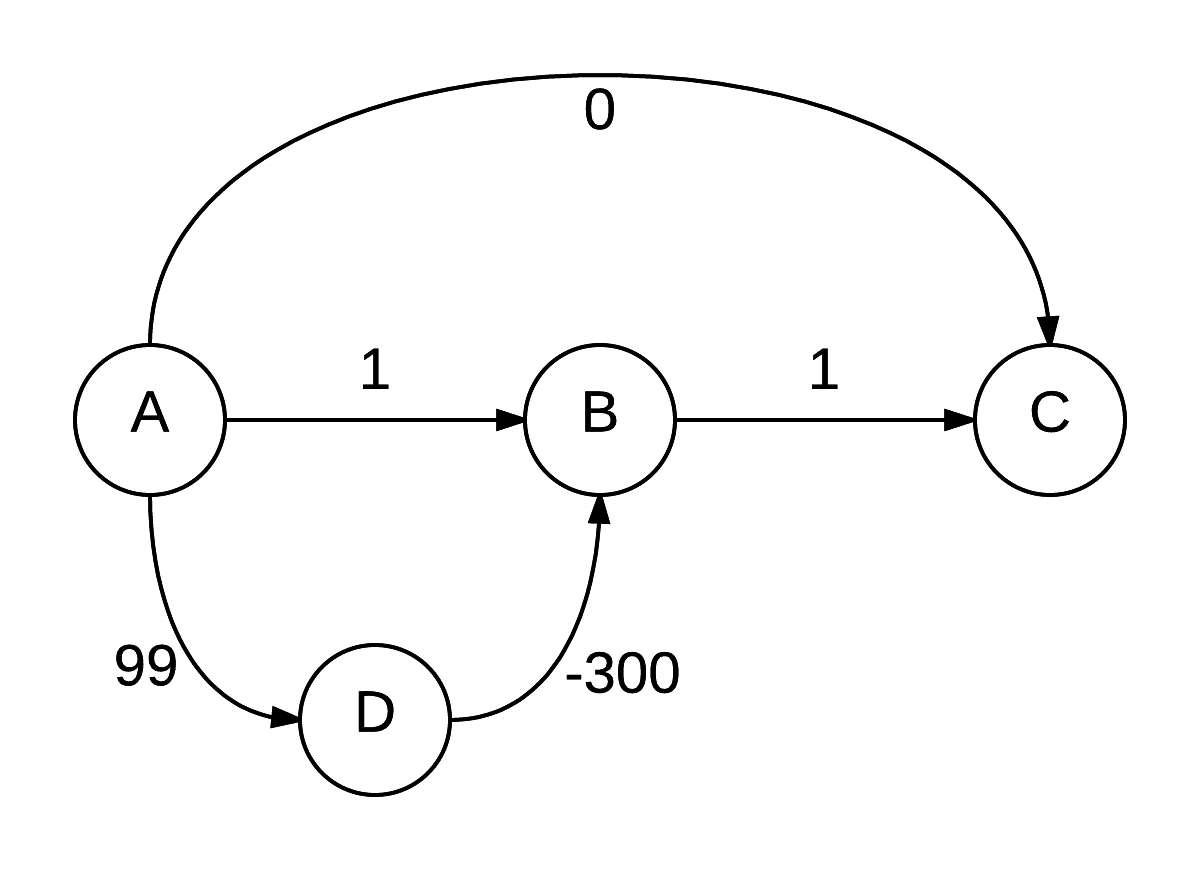
\includegraphics[width=6cm]{bfex}
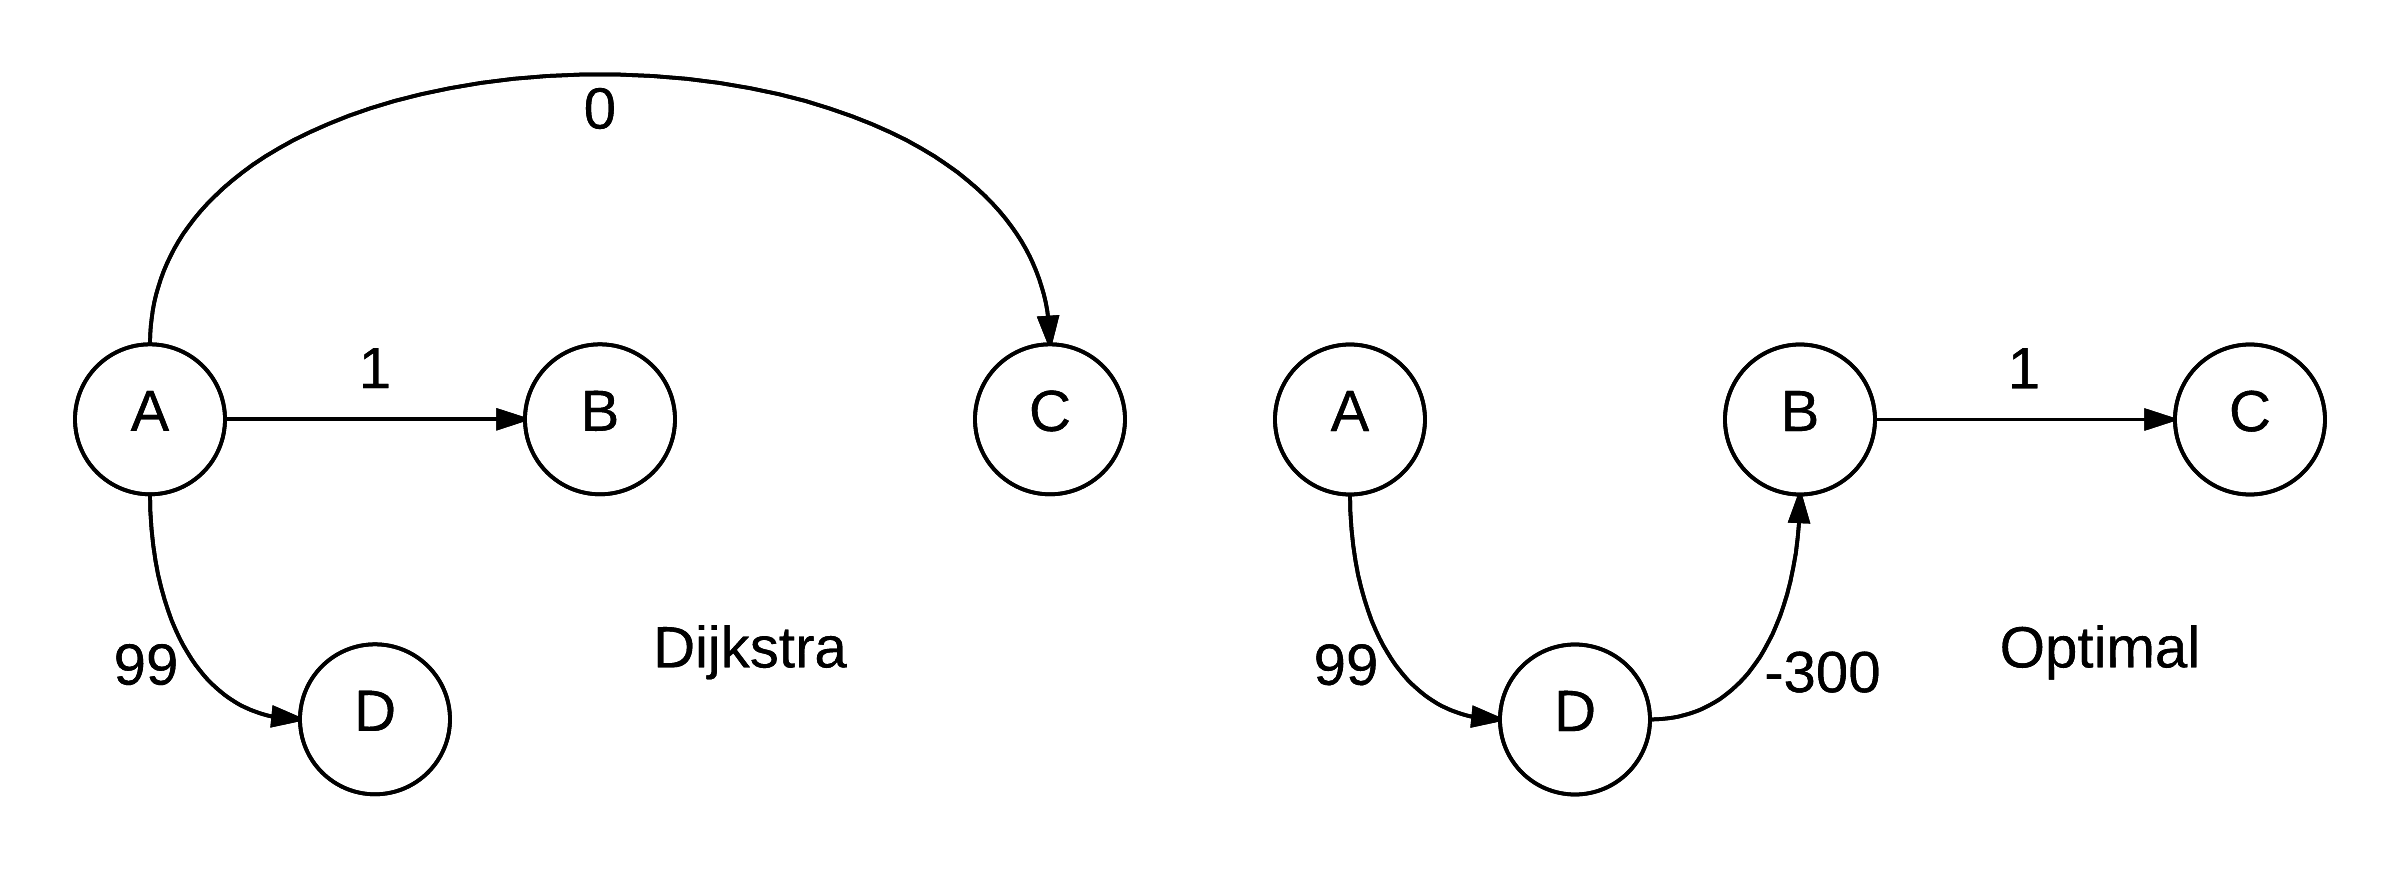
\includegraphics[width=12cm]{bfcd}
\end{figure}
\FloatBarrier
Considering the shortest paths with negative weights adds other additional constraints:
\begin{itemize}
\item The problem makes sense iff there are no cycles with negative weight.
\item The graph must be directed else even one negative edge may create this undesirable effect.
\item Consider a graph G without negative cycles. If a node v is reachable from the source then the shortest path has length (number of hops) less than n.
\end{itemize}

\paragraph{Proof:} Assuming there is a shortest path p with length $\geq$ n. This implies that there must exist in the path, a cycle. Iff that cycle is negative, then w(p)$<$w(p'). Without negative weighted edges, and cycles, this would be impossible.
\begin{figure}[h]
\centering
\includegraphics[width=10cm]{negcycles}
\end{figure}
\subsection{Dynamic Programming Approach}
\begin{itemize}
\item Define subproblems by considering shortest paths of at most length k:k=[0..n]
\item Define a table M, of size k$\times$v
\item M[k,v] is the weight of the shortest path between the source s and v of at most length k if there exists a path of length less than or equal to k. M[k,v] equals infinity otherwise. 
\item Base case:k=0 $\to$ M[0,s]=0 and M[0,v]=$\infty\forall v\neq s$
\item In general, for all k and v:
\[M[k,v]=\begin{cases}M[k-1,v] & \nexists\text{ shorter path}\\ M[k-1,u]+w(u,v)\forall u \in adj(v)& \exists\text{ shorter path}\end{cases}\]
\item M[k,v]=min(M[k-1,v],min(M[k-1,u]+w(u,v):(u,v)$\in$ E))
\item If $\exists v: M[n,v]\neq M[n-1,v]\to \exists$ negative cycles
\end{itemize}
Refering to the earlier graph for which Dijkstra's algorithm yielded a non-optimal solution, consider the following table illustrating the execution of the Bellman-Ford algorithm.
\begin{figure}
\centering
\begin{tabular}{|c|c|c|c|c|}
\hline
 &A&B&C&D\\ \hline \hline
0&0&$\infty$&$\infty$&$\infty$\\ \hline
1&0&1&0&99\\ \hline
2&0&-201&0&99\\ \hline
3&0&-201&-200&99\\ \hline
4&0&-201&-200&99\\ \hline
\end{tabular}
\caption{Table for the Bellman-Ford execution on the earlier graph example opening this section}
\end{figure}
Consider the following graph which is simple, but obviously contains a negative cycle and the following table illustrating the change earlier asserted as indicative of the presence of a negative cycle. 
\begin{figure}[h]
\centering
\includegraphics[width=4cm]{negcycleex}
\begin{tabular}{|c|c|c|c|}
\hline
 &A&B&C \\ \hline \hline
0&0&$\infty$&$\infty$\\ \hline
1&0&1&$\infty$\\ \hline
2&0&1&3\\ \hline
3&\textbf{-1}& & \\ \hline
\end{tabular}
\end{figure}

\end{document}